%\documentclass{article}

\documentclass{article} % For LaTeX2e
\usepackage{iclr2025_conference,times}

% Optional math commands from https://github.com/goodfeli/dlbook_notation.
\input{math_commands.tex}

% \usepackage{hyperref}
% \usepackage{url}

% if you need to pass options to natbib, use, e.g.:
%     \PassOptionsToPackage{numbers, compress}{natbib}
% before loading neurips_2024


% ready for submission
%\usepackage{neurips_2024}


% to compile a preprint version, e.g., for submission to arXiv, add add the
% [preprint] option:
%\usepackage[preprint]{neurips_2024}


% to compile a camera-ready version, add the [final] option, e.g.:
%     \usepackage[final]{neurips_2024}


% to avoid loading the natbib package, add option nonatbib:
%    \usepackage[nonatbib]{neurips_2024}


\usepackage[utf8]{inputenc} % allow utf-8 input
\usepackage[T1]{fontenc}    % use 8-bit T1 fonts
\usepackage{hyperref}       % hyperlinks
\usepackage{url}            % simple URL typesetting
\usepackage{booktabs}       % professional-quality tables
\usepackage{amsfonts}       % blackboard math symbols
\usepackage{nicefrac}       % compact symbols for 1/2, etc.
\usepackage{microtype}      % microtypography
\usepackage{xcolor}         % colors


\usepackage{multirow}
\usepackage{wrapfig}

\usepackage{graphics}
\usepackage{graphicx}
\usepackage{amsmath}
\usepackage{wrapfig}
\usepackage[subfigure]{tocloft}
\usepackage{subcaption}
\usepackage{amsfonts,bm,amssymb}
\usepackage{natbib} 

\usepackage{macros}
% \usepackage{algorithm}
% \usepackage{algorithmic}
% \usepackage{float}  % For math environments and symbols Ensure the 'H' position specifier is available
\usepackage{algorithm}
%\usepackage{algorithmic}

\usepackage{algpseudocode}
\usepackage{amsmath}
\usepackage{float}
\usepackage{multicol}
\usepackage{setspace}

% \usepackage{tikz}
% \usetikzlibrary{shapes.geometric, arrows}

\usepackage{tikz}
\usetikzlibrary{shapes.geometric, arrows}

\tikzstyle{startstop} = [rectangle, rounded corners, minimum width=3cm, minimum height=1cm,text centered, draw=black, fill=red!30]
\tikzstyle{process} = [rectangle, minimum width=3cm, minimum height=1cm, text centered, draw=black, fill=blue!30]
\tikzstyle{decision} = [diamond, minimum width=3cm, minimum height=1cm, text centered, draw=black, fill=green!30]
\tikzstyle{arrow} = [thick,->,>=stealth]

 \usepackage{tabularray}
 \usepackage{multirow}

\usepackage[inline]{enumitem}

%\usepackage{algorithm2e}
% \usepackage{amsmath}

%%%%% UPDATE CITE %%%%%
%\usepackage{etoolbox}
%\usepackage[numbers]{natbib}


% \makeatletter
% \patchcmd{\@citex}{\@citeo}{[{#1\if@tempswa , #2\fi}]}{}{}
% \makeatother
\renewcommand{\cite}[1]{\citep{#1}}

%%%%% %%%%% %%%%% %%%%%

\newcommand{\xref}[1]{\S\ref{#1}}
\newcommand{\dc}[1]{{\textcolor{red}{#1}}}
%\newcommand{\dc}[1]{\COMMENT{\textcolor{red}{\sf Deeksha says: #1}}}
\newcommand{\jack}[1]{{\textcolor{blue}{#1}}}
%\newcommand{\fixme}[1]{{\textcolor{orange}{#1}}}

%\title{NExUME: Revisiting DNN Training for Intermittently-Powered Energy-Harvesting Wireless Sensor Network}

%\title{Revisiting DNN Training for Intermittently-Powered Energy-Harvesting Micro-Computers}
%\title{NExUME: Adaptive Training and Inference for Deep Neural Networks under Intermittent Power Environments}
% \title{Adaptive Training and Inference for DNNs under Intermittent Power Environments}
\title{NExUME: Adaptive Training and Inference for DNNs under Intermittent Power Environments}
% The \author macro works with any number of authors. There are two commands
% used to separate the names and addresses of multiple authors: \And and \AND.
%
% Using \And between authors leaves it to LaTeX to determine where to break the
% lines. Using \AND forces a line break at that point. So, if LaTeX puts 3 of 4
% authors names on the first line, and the last on the second line, try using
% \AND instead of \And before the third author name.


% \author{%
% Cyan Subhra Mishra, Deeksha Chaudhary, Jack Sampson, Mahmut Taylan Knademir, Chita Das\\
% \texttt{CSE Department, The Pennsylvania State University}\\
% \texttt{\{cyan, dmc6955, jms1257, mtk2, cxd12\}@psu.edu}
% }
% \author{%
% Cyan Subhra Mishra, Deeksha Chaudhary, Jack Sampson, Mahmut Taylan Knademir, Chita Das\\
% \texttt{CSE Department, The Pennsylvania State University}\\[2mm]
% \href{mailto:cyan@psu.edu}{\texttt{cyan@psu.edu}}, 
% \href{mailto:dmc6955@psu.edu}{\texttt{dmc6955@psu.edu}}, 
% \href{mailto:jms1257@psu.edu}{\texttt{jms1257@psu.edu}}, 
% \href{mailto:mtk2@psu.edu}{\texttt{mtk2@psu.edu}}, 
% \href{mailto:cxd12@psu.edu}{\texttt{cxd12@psu.edu}}
% }

\author{%
Cyan Subhra Mishra, Deeksha Chaudhary, Jack Sampson, Mahmut Taylan Knademir, Chita Das\\
\texttt{CSE Department, The Pennsylvania State University}\\[2mm]
\texttt{\{}\href{mailto:cyan@psu.edu}{cyan}, \href{mailto:dmc6955@psu.edu}{dmc6955}, \href{mailto:jms1257@psu.edu}{jms1257}, \href{mailto:mtk2@psu.edu}{mtk2}, \href{mailto:cxd12@psu.edu}{cxd12}\texttt{\}@psu.edu}
}

\iclrfinalcopy
\begin{document}
\maketitle
%%%%%%%%%%%%%%%%%%%%%%%%%%%%%%%%%%%%%%%%%%%%%%%%%%%
%\begin{abstract}
%%%%%

% The deployment of Deep Neural Networks (DNNs) in energy-constrained environments, such as Energy Harvesting Wireless Sensor Networks (EH-WSNs), presents unique challenges, primarily due to the ``intermittent'' nature of power availability. To address these challenges, this study introduces and evaluates a novel training methodology tailored for DNNs operating within such contexts. In particular, we propose a dynamic dropout technique that adapts to both the architecture of the device and the variability in energy availability inherent in energy harvesting scenarios. 

% Our proposed approach leverages a device model that incorporates specific parameters of the network architecture and the energy harvesting profile to optimize dropout rates dynamically during the training phase. By modulating the network’s training process based on predicted energy availability, our method not only conserves energy but also ensures sustained learning and inference capabilities under power constraints. Our preliminary results demonstrate that this strategy provides $6\%$ -- $22\%$ accuracy improvements compared to the state of the art with $\le 5\%$ additional compute. This paper details the development of the device model, describes the integration of energy profiles with intermittency aware dropout and quantization algorithms, and presents a comprehensive evaluation  of the proposed approach using real-world energy harvesting data. The work also includes a new dataset towards deploying energy harvesting based computation in real world.
\begin{abstract}
The deployment of Deep Neural Networks (DNNs) in energy-constrained environments, such as Energy Harvesting Wireless Sensor Networks (EH-WSNs), introduces significant challenges due to the intermittent nature of power availability. This study introduces \textit{NExUME}, a novel training methodology designed specifically for DNNs operating under such constraints. We propose a dynamic adjustment of training parameters---dropout rates and quantization levels---that adapt in real-time to the available energy, which varies in energy harvesting scenarios. 

This approach utilizes a model that integrates the characteristics of the network architecture and the specific energy harvesting profile. It dynamically adjusts training strategies, such as the intensity and timing of dropout and quantization, based on predictions of energy availability. This method not only conserves energy but also enhances the network’s adaptability, ensuring robust learning and inference capabilities even under stringent power constraints. Our results show a 6\% to 22\% improvement in accuracy over current methods, with an increase of less than 5\% in computational overhead. This paper details the development of the adaptive training framework, describes the integration of energy profiles with dropout and quantization adjustments, and presents a comprehensive evaluation using real-world data. Additionally, we introduce a novel dataset aimed at furthering the application of energy harvesting in computational settings.
\end{abstract}

%%%%%


%\end{abstract}
%%%%%%%%%%%%%%%%%%%%%%%%%%%%%%%%%%%%%%%%%%%%%%%%%%%

%%%%%%%%%%%%%%% CONTENT STARTS HERE %%%%%%%%%%%%%%%

%%%%%%%%%%%%%%%%%%%%%%%%%%%%%%%%%%%%%%%%%%%%%%%%%%%
\section{Introduction}
%% %%%%% %%%%% %%%%%
% The proliferation of Internet of Things (IoT) devices in diverse and challenging environments—such as wildlife monitoring~\cite{tuia2022perspectives,gobieski2019intelligence}, deep mine surveillance~\cite{bai2020real, ni2024detection}, and remote industrial automation~\cite{visconti2024machine, khalil2021deep}—demands efficient and reliable image classification~\cite{RedEye2020, qiu2020resirca}. These applications often operate under stringent energy constraints, requiring ultra-low power consumption, long device lifetimes, and minimal maintenance~\cite{qiu2020resirca, gobieski2019intelligence}. For example, wildlife monitoring sensors must often run for years without battery replacements, and deep-mine surveillance systems face hostile environments where frequent maintenance is infeasible. Energy-harvesting technologies are increasingly being leveraged to meet these requirements, enabling devices to operate indefinitely, but intermittently~\cite{Lv2022, qiu2020resirca, ma2017incidental}.  In such contexts, traditional image classification solutions fall short due to their significant energy overhead~\cite{RedEye2020, IMBNature}, necessitating novel paradigms for energy-efficient computing.

% Amongst these approaches, Processing-in-Memory (PIM) architectures have emerged as a transformative solution, 
% %for these constraints
% with Resistive RAM (ReRAM)--based crossbars (xBars) demonstrating particular promise, especially for DNN-based inference serving~\cite{shafiee2016isaac}. xBars excel in their ability to perform matrix-vector multiplications (MVMs) directly in the analog domain, drastically reducing the energy overhead of data movement and digital processing~\cite{reramNature, chi2016prime, shafiee2016isaac, singh2020nebula}. A typical image inference pipeline using ReRAM crossbars is depicted in Figure~\ref{fig:IntroDiagram}. Data from image sensors are stored in the memory (often an eDRAM)~\cite{singh2020nebula, shafiee2016isaac, chi2016prime} and part of the multiply-accumulate functionality of the DNN execution is performed in the crossbar. 
% Finally, the activation functions and data-flow orchestration are typically managed by an microcontroller unit (MCU) or a dedicated control block.

% Furthermore, the non-volatility and endurance of ReRAM make it particularly suitable for low-power scenarios, where reliability over extended lifetimes is paramount~\cite{chen2020reram, rizk2019demystifying}. 
% In addition, compatibility with existing CMOS fabrication processes further enhances the commercial viability of ReRAM-based systems~\cite{IMBNature}.

% \begin{figure}[t]
%     \centering
%     \includegraphics[width=\linewidth]{figs/RichIntroDiagram.pdf}
%     \vspace{-22pt}\caption {An example wildlife classification deployment - Analog image sensor data is stored in digital memory, then  processed in crossbar arrays in the mixed domain. The MCU, in the digital domain, performs activation functions. Every DNN layer undergoes expensive domain transfers.}
%     \label{fig:IntroDiagram}
% \end{figure}


% Despite these advantages, significant challenges remain in deploying ReRAM-based systems for ultra low-power and energy-harvesting environments. A critical limitation is the energy and latency overheads associated with analog-to-digital (A2D) and digital-to-analog (D2A) conversions~\cite{shafiee2016isaac, singh2020nebula}. As depicted in Figures~\ref{fig:IntroDiagram} and~\ref{fig:xbarFlow}, in a typical image inference flow, the matrix-vector multiplication (MVM) computations happen in the crossbar arrays operating in the analog domain, while the activation functions, control management, and memory management are performed in the digital domain~\cite{shafiee2016isaac, singh2020nebula, chi2016prime, qiu2020resirca}. After performing MVM, each layer in a DNN typically needs to execute a nonlinear activation function, particularly the rectified linear unit (ReLU)~\cite{lecun1998gradient, hahnloser2000digital, hahnloser2000correction}, which is indispensable for modern neural networks~\cite{howard2017mobilenets}. Although activation computations are generally inexpensive, they are typically done off-crossbar and require A2D conversion~\cite{shafiee2016isaac}, leading to frequent A2D and D2A conversions. These conversions can consume up to $82\%$ of the power and $31\%$ of the area~\cite{shafiee2016isaac, chi2016prime, IMBNature}, severely undermining the efficiency gains of the PIM architecture. Traditional designs often offload these activation computations to external digital processors, such as microcontroller units (MCUs)~\cite{singh2020nebula, qiu2020resirca} or specialized digital circuits~\cite{IMBNature}, which not only incurs additional energy and latency costs but also undermines the core advantage of PIM architectures by requiring frequent data movement between analog crossbars and digital processing units. For instance, each off-crossbar activation processing step can add a latency overhead of $15\%$ to $18\%$ and contribute approximately $5\%$ to the total energy budget in ultra-low-power systems~\cite{shafiee2016isaac, chi2016prime, IMBNature}.

% Another significant issue is the degradation of computational accuracy due to IR drops and other analog noise/variability in large-scale crossbar arrays. Since the crossbar computation is entirely based on Ohmic properties, the voltage drop across stages causes an uneven distribution of voltage within the crossbar. This leads to reduced fidelity in analog computations, with accuracy drops of up to $25\%$ reported in certain configurations~\cite{IRDropDAC, IRDropTCAD, lee2024mitigating}. 
% Mitigation strategies, such as current balancing and the inclusion of intermediate storage registers, exacerbate energy consumption, often increasing the overall power budget~\cite{crafton2022characterization, IRDropICCD}. Furthermore, traditional neural network models are often designed without consideration of the non-idealities inherent in analog hardware. Hardware-induced noise, variability in device characteristics, and diverse operating conditions can lead to significant performance degradation, particularly in scenarios with tight energy budgets and low data fidelity~\cite{lee2024mitigating, IRtrainingBL}. For example, analog noise can introduce errors that degrade classification accuracy by $15\%$ if not properly accounted for in the network design~\cite{singh2020nebula}.

% To address these challenges, we advocate for the co-optimization of model architectures and hardware configurations, a strategy that remains underexplored. Current designs often fail to consider how tile sizes, data representations, and hardware resources interact to impact overall energy efficiency and performance in low-power xBars. Although recent work has explored adaptive tiling strategies~\cite{qiu2020resirca}, they lack joint optimization of neural networks and PIM architectures. Such co-design strategies are critical for unlocking the full potential of ReRAM-based accelerators in ultra-low-power and energy-harvesting systems.
% In this paper, we address these challenges by proposing a novel framework that integrates \emph{hardware-aware neural network design} and \emph{energy-efficient activation strategies}. Our approach bridges the gap between hardware limitations and neural network requirements, delivering practical solutions for deploying ReRAM-based systems in energy-constrained environments. Our experimental results demonstrate up to \textbf{68\%} improvement in energy efficiency and \textbf{25\%} reduction in latency, allowing robust image classification for applications such as wildlife monitoring and industrial automation under strict energy constraints. The \textbf{key contributions} of this paper are as follows:

% \noindent$\bullet$ \textbf{Analog Activation with Schottky Diodes:} We present a novel analog activation function implemented using Schottky diodes, which offer low voltage drop, rapid switching and minimal leakage. This eliminates the need for off-chip or off-crossbar digital activation processing, reducing energy consumption and latency while ensuring seamless compatibility with analog crossbar operations.

% \noindent$\bullet$ \textbf{Hardware-Aware Training:} Our training pipeline incorporates real-world hardware non-idealities to enhance robustness and efficiency. We introduce an activation function that models Schottky diode behavior in the analog domain, enabling the neural network to adapt to hardware constraints during training. We also design a loss function that accounts for IR drop and hardware noise profiles, resulting in models resilient to voltage fluctuations and analog noise—critical factors in ultra low-power applications.

% \noindent$\bullet$ \textbf{Model-Hardware Co-Design:} We adopt a co-design strategy that simultaneously optimizes the DNN and hardware architecture for superior energy efficiency and performance. Key innovations include a tile-based architecture that allows parallel analog computations within crossbar arrays and the ability to compute two consecutive neural network layers entirely in the analog domain. Additionally, during training, techniques such as tile dropout are employed to boost model robustness against real-world challenges like incomplete or noisy data.

% \noindent$\bullet$ \textbf{Comprehensive Evaluation:} We conduct extensive evaluations to validate the proposed system. Our results demonstrate significant improvements over state-of-the-art methods, achieving up to \textbf{68\%} energy savings and \textbf{25\%} latency reductions while maintaining high classification accuracy. Specifically, on benchmark datasets, our analog-aware trained models maintain high classification accuracy, achieving up to \textbf{1.63\%} improvement over 4-bit quantized models. In a case study using the NTLNP wildlife image dataset~\cite{ntlnpdataset, tan2022animal, ntlnprepo}, our system achieves an accuracy of \textbf{88.1\%} with MicroNet, outperforming the 4-bit baseline by \textbf{4.9\%} and RedEye by \textbf{6.06\%}, highlighting the versatility and practicality of our solution. \textcolor{blue}{We further expand our evaluations on modern transformer based architectures to show generalization of the new activation function.}

% \textcolor{blue}{To the best of our knowledge, this is the first work to integrate hardware-aware training, 
% an analog activation circuit based on Schottky diodes, 
% and a comprehensive model--hardware co-design \emph{specifically} for \textbf{ReRAM}-based PIM architectures.}
% By bridging the gap between neural network design and analog hardware constraints, our approach enables robust and energy-efficient image classification tailored for ultra-low-power and edge systems.
% %%%%% %%%%% %%%%%

%%%%%%%%%%%%%%%%%%%%%%%%%%%%%%%%%%%%%%%%%
%%%%%%%%%%%%%%%%%%%%%%%%%%%%%%%%%%%%%%%%%

 \section{Introduction}
\label{sec:intro}

The rapid proliferation of Internet of Things (IoT) devices in diverse and often hostile environments—such as wildlife monitoring~\cite{tuia2022perspectives,gobieski2019intelligence}, deep mine surveillance~\cite{bai2020real, ni2024detection}, and remote industrial automation~\cite{visconti2024machine, khalil2021deep}—demands \emph{efficient} and \emph{reliable} image classification solutions~\cite{RedEye2020, qiu2020resirca}. These applications characteristically operate under stringent energy constraints, where ultra-low power consumption, extended device lifetimes, and minimal maintenance are paramount~\cite{qiu2020resirca, gobieski2019intelligence}. For instance, wildlife monitoring sensors may need to run for years in remote habitats without battery replacements, while deep-mine surveillance nodes must withstand harsh conditions that render frequent maintenance impractical. To address these limitations, energy-harvesting technologies are increasingly employed, enabling devices to operate \emph{indefinitely} but often \emph{intermittently}~\cite{Lv2022, qiu2020resirca, ma2017incidental}. Under such conditions, traditional image classification approaches—usually reliant on power-hungry digital processing—fail to meet the rigorous energy constraints~\cite{RedEye2020, IMBNature}, thus demanding novel paradigms for \emph{energy-efficient computing}.

One promising line of research for achieving such efficiency targets is \emph{Processing-in-Memory} (PIM) architectures, particularly those that leverage \emph{Resistive RAM} (ReRAM) crossbars (xBars) for DNN-based inference~\cite{shafiee2016isaac}. Unlike standard digital designs, ReRAM xBars perform matrix-vector multiplications (MVMs) \emph{directly} in the analog domain, significantly reducing the energy overhead of data movement and digital processing~\cite{reramNature, chi2016prime, shafiee2016isaac, singh2020nebula}. Figure~\ref{fig:IntroDiagram} illustrates a typical image inference pipeline wherein data from image sensors are stored in memory (often eDRAM)~\cite{singh2020nebula, shafiee2016isaac, chi2016prime}, and a portion of the multiply-accumulate operations is offloaded to analog crossbars. Subsequently, activation functions and data-flow orchestration are conventionally managed by a microcontroller unit (MCU) or a dedicated control block. Further strengthening the prospects of ReRAM, its non-volatility and high endurance make it particularly suited for long-term reliability in low-power scenarios~\cite{chen2020reram, rizk2019demystifying}, and its compatibility with existing CMOS fabrication processes elevates its commercial viability~\cite{IMBNature}.

\begin{figure}[t]
    \centering
    \includegraphics[width=\linewidth]{figs/RichIntroDiagram.pdf}
    \vspace{-22pt}
    \caption{An example wildlife classification deployment---analog image sensor data is stored in digital memory, then processed in crossbar arrays in the mixed domain. The MCU, in the digital domain, performs activation functions. Every DNN layer undergoes expensive domain transfers.}
    \label{fig:IntroDiagram}
\end{figure}

Despite these notable advantages, significant hurdles remain in deploying ReRAM-based PIM systems for ultra low-power and intermittently powered settings. A primary challenge is the steep energy and latency overhead of analog-to-digital (A2D) and digital-to-analog (D2A) conversions~\cite{shafiee2016isaac, singh2020nebula}. As depicted in Figures~\ref{fig:IntroDiagram} and~\ref{fig:BaseArch}\textit{(I)}, while crossbar arrays compute MVM in the analog domain, crucial tasks such as activation functions, memory management, and control logic typically occur in the digital domain~\cite{shafiee2016isaac, singh2020nebula, chi2016prime, qiu2020resirca}. Modern DNNs rely heavily on nonlinear activations, particularly rectified linear units (ReLUs)~\cite{lecun1998gradient, hahnloser2000digital, hahnloser2000correction}, for boosting network performance~\cite{howard2017mobilenets}. Although the activation calculations themselves are often computationally light, the off-crossbar requirement for digital processing triggers frequent A2D and D2A conversions~\cite{shafiee2016isaac}, which can consume up to $82\%$ of the total power and occupy $31\%$ of the die area~\cite{shafiee2016isaac, chi2016prime, IMBNature}. Typical solutions offload these computations to external MCUs~\cite{singh2020nebula, qiu2020resirca} or specialized digital hardware~\cite{IMBNature}, but this offloading undercuts the central advantage of PIM—eliminating most data movement—and further inflates energy and latency. Notably, each off-crossbar activation step can add $15\%$ to $18\%$ latency overhead and approximately $5\%$ extra energy budget in ultra-low-power implementations~\cite{shafiee2016isaac, chi2016prime, IMBNature}.

Moreover, computational accuracy in analog crossbars suffers from IR drops and device-level variations inherent to large-scale arrays. Because crossbar computations hinge on Ohmic properties, voltage drop across rows and columns leads to uneven signal distribution, culminating in accuracy losses of up to $25\%$ in certain setups~\cite{IRDropDAC, IRDropTCAD, lee2024mitigating}. Existing mitigation techniques—ranging from current balancing to insertion of intermediate storage registers—amplify energy usage and degrade overall efficiency~\cite{crafton2022characterization, IRDropICCD}. Complicating matters, mainstream DNN architectures are typically designed with digital hardware assumptions, disregarding analog noise, device variability, and constrained precision in crossbars~\cite{lee2024mitigating, IRtrainingBL}. Such mismatch can introduce classification errors exceeding $15\%$~\cite{singh2020nebula} if models are not adapted to the underlying analog realities—an unacceptable performance drop for mission-critical or resource-starved applications.

To surmount these obstacles, we underscore the importance of jointly optimizing model architectures and hardware configurations. Few existing solutions fully account for how tile sizes, data representations, and analog hardware constraints interplay to affect energy efficiency and accuracy, particularly in ultra-low-power ReRAM designs~\cite{qiu2020resirca}. Although adaptive tiling has been explored, most lack comprehensive co-design of both the neural network and PIM architecture. Bridging this gap is paramount for extracting the full performance and energy gains that ReRAM crossbars can offer in edge deployments.

In this paper, we propose a novel framework that integrates \emph{hardware-aware neural network design} with \emph{energy-efficient activation strategies}, delivering a holistic solution for deploying ReRAM-based systems under tight energy budgets. Our approach confronts the dual constraints of analog non-idealities and constrained power budgets, achieving \textbf{up to 68\%} improvement in energy efficiency and \textbf{25\%} reduction in latency. These gains enable robust, continuous image classification for domains like wildlife monitoring and industrial automation, even under intermittent or harvested power. The \textbf{key contributions} of this paper include:

\begin{itemize}[leftmargin=*]
    \item \textbf{Analog Activation with Schottky Diodes:} We propose a novel analog activation function employing Schottky diodes, which feature low forward voltage drop, rapid switching speeds, and negligible leakage. This design obviates the need for off-chip or off-crossbar digital activations, cutting energy consumption and latency while preserving seamless compatibility with analog crossbar operations.
    
    \item \textbf{Hardware-Aware Training:} We build a training pipeline that explicitly incorporates real-world hardware non-idealities. By modeling Schottky diode dynamics and IR drop behavior in the activation function, we enable the DNN to adapt to analog-domain constraints. We further incorporate hardware noise profiles into the loss function, ensuring that trained models remain robust against voltage fluctuations and noise—pivotal in ultra low-power applications.
    
    \item \textbf{Model-Hardware Co-Design:} Our approach enforces a co-design paradigm wherein DNN architectures and the underlying ReRAM xBar hardware are optimized in tandem. We introduce a tile-based design to facilitate parallel analog MVMs across crossbar arrays, and exploit the potential to compute two consecutive network layers entirely in the analog domain. 
    %Furthermore, we apply \emph{tile dropout} techniques during training to bolster the model’s resilience against partial or noisy data, a common occurrence in energy-scarce environments.
    
    \item \textbf{Comprehensive Evaluation:} We conduct extensive validations to gauge the effectiveness of our framework against state-of-the-art references, observing up to \textbf{68\%} energy savings and \textbf{25\%} latency reductions, all while preserving high classification accuracy. Specifically, across standard benchmarks, our analog-aware models yield up to \textbf{1.63\%} higher accuracy compared to 4-bit quantized networks. Furthermore, on the NTLNP wildlife image dataset~\cite{ntlnpdataset, tan2022animal, ntlnprepo}, our method achieves an \textbf{88.1\%} accuracy using MicroNet, surpassing the 4-bit baseline by \textbf{4.9\%} and outperforming RedEye by \textbf{6.06\%}. We also extend our evaluation to modern transformer-based architectures, underscoring our activation function’s broad applicability.
\end{itemize}

To the best of our knowledge, this is the first comprehensive approach to integrate hardware-aware training, a Schottky diode-based analog activation circuit, and a model--hardware co-design specifically tailored to \textbf{ReRAM}-based PIM accelerators. By reconciling neural network design with the realities of analog crossbar hardware, our strategy achieves \emph{robust, energy-efficient} image classification suitable for ultra-low-power and edge deployments.


% %%%%%%%%%%%%%%%%%%%%%%%%%%%%%%%%%%%%%%%%%%%
% %%%%%%%%%%%%%%%%%%%%%%%%%%%%%%%%%%%%%%%%%%%
% \section{Introduction}
% \label{sec:intro}

% The rapid expansion of Internet of Things (IoT) devices in diverse, often harsh environments—such as wildlife monitoring~\cite{tuia2022perspectives,gobieski2019intelligence}, deep-mine surveillance~\cite{bai2020real, ni2024detection}, and remote industrial automation~\cite{visconti2024machine, khalil2021deep}—has created a pressing need for highly \emph{energy-efficient} and \emph{robust} image classification solutions~\cite{RedEye2020, qiu2020resirca}. These deployment scenarios typically demand ultra-low-power consumption and minimal maintenance over extended timeframes~\cite{gobieski2019intelligence, qiu2020resirca}, with devices often operating on tightly constrained power budgets or intermittent energy-harvesting schemes~\cite{Lv2022, qiu2020resirca, ma2017incidental}. For instance, wildlife monitoring sensors in remote forests must run continuously for years with limited battery replacements, and deep-mine surveillance systems may have to withstand extreme temperatures, physical obstructions, and hazardous conditions with infrequent recharges.

% In pursuit of these stringent requirements, \emph{Processing-in-Memory} (PIM) architectures based on \emph{Resistive RAM} (ReRAM) crossbars (xBars) have emerged as a transformative solution for deep neural network (DNN) inference~\cite{shafiee2016isaac, chi2016prime, singh2020nebula}. ReRAM xBars directly execute matrix-vector multiplications (MVMs) in the analog domain, mitigating energy overheads associated with data movement and memory accesses~\cite{reramNature, singh2020nebula}. Their non-volatile nature and compatibility with modern CMOS processes further bolster their suitability for embedded and edge AI~\cite{chen2020reram, rizk2019demystifying, IMBNature}. Figure~\ref{fig:IntroDiagram} depicts a typical ReRAM-based image inference pipeline in which analog operations (e.g., partial multiply-accumulate computations) occur inside crossbar arrays, while a microcontroller or specialized digital block handles activation functions and orchestrates the data flow.

% Despite these advantages, realizing \emph{fully analog inference} at ultra-low-power faces three critical challenges. First, frequent analog-to-digital (A2D) and digital-to-analog (D2A) conversions—required each time intermediate results or activations move between analog and digital domains—can consume up to $82\%$ of the overall power and $31\%$ of the area in PIM accelerators~\cite{shafiee2016isaac, chi2016prime, IMBNature}. Second, large-scale crossbar arrays suffer from IR drops and inherent hardware noise, triggering notable accuracy degradation if the network is not tailored to these analog non-idealities~\cite{IRDropDAC, IRDropTCAD, lee2024mitigating, IRDropICCD}. Third, many prior approaches lack a holistic co-design framework that \emph{simultaneously} optimizes both the DNN model and the underlying PIM hardware, missing opportunities to leverage tile-level parallelism, reduce conversion overheads, and incorporate real device parameters into training~\cite{qiu2020resirca, singh2020nebula}.

% In this paper, we tackle these gaps by introducing a comprehensive framework that unifies \emph{hardware-aware neural network training} with \emph{energy-efficient analog activation} in ReRAM xBars. Specifically, we replace the conventional digital off-chip activation with a Schottky-diode-based analog activation module, dramatically reducing cross-domain conversions. We further strengthen our \emph{co-design methodology} to account for hardware noise, IR drops, and intermittent power scenarios, and we experimentally validate our approach on both classic network architectures and emerging transformer-based designs. Our key contributions are as follows:

% \begin{itemize}[leftmargin=*]
%     \item \textbf{Analog Activation via Schottky Diodes:} We propose a novel analog activation circuit leveraging Schottky diodes for low forward voltage drop, rapid switching, and minimal leakage current. By embedding the non-linear activation directly in the analog domain, our design avoids repeated A2D/D2A conversions, substantially cutting energy and latency costs.
%     %
%     \item \textbf{Hardware-Aware Training:} We incorporate Schottky diode characteristics and crossbar-specific non-idealities (e.g., IR drop, device variability, and noise) into the training pipeline. The resulting networks are \emph{analog-aware}—they learn to maintain high classification accuracy under the voltage and signal distortions endemic to ReRAM crossbars, which is vital in ultra-low-power deployments.
%     %
%     \item \textbf{Model--Hardware Co-Design:} Beyond analog activations, we outline a tile-based crossbar architecture that processes two consecutive DNN layers fully in analog, reducing back-and-forth domain transfers. Techniques like \emph{tile dropout} bolster resilience to partial node failures or incomplete powering in energy-harvesting systems. This joint optimization of model topology and hardware resources closes the gap between analog capabilities and DNN requirements.
%     %
%     \item \textbf{Comprehensive Evaluation:} We extensively evaluate our framework on multiple benchmarks, including wildlife images~\cite{ntlnpdataset, tan2022animal, ntlnprepo} and transformer-based models. Our analog-aware networks achieve up to \textbf{68\%} energy savings and \textbf{25\%} latency reductions compared to state-of-the-art baselines, while maintaining—and in some cases improving—top-1 accuracy by up to \textbf{4.9\%} over a 4-bit quantized baseline in real-world scenarios.
% \end{itemize}

% \begin{figure}[t]
%     \centering
%     \includegraphics[width=\linewidth]{figs/RichIntroDiagram.pdf}
%     \caption{An example wildlife classification deployment. Analog image sensor data are stored in on-chip memory, partially processed via ReRAM crossbars, and then passed to an MCU for data orchestration. In typical designs, frequent cross-domain transfers for activation functions incur significant overheads. By embedding analog activations, our approach reduces these energy and latency bottlenecks.}
%     \label{fig:IntroDiagram}
% \end{figure}

% \noindent \textbf{Significance.} To the best of our knowledge, this is the first work to \emph{jointly} introduce a Schottky-diode-based analog activation design, a robust hardware-aware training flow, and a holistic model--hardware co-design specifically tailored for ReRAM-based PIM accelerators. By aligning the network’s structure with real-world device behavior, our solution not only maximizes energy efficiency but also maintains accuracy under power-scarce and noisy conditions, thus paving the way for next-generation ultra-low-power IoT deployments.

% %%%%%%%%%%%%%%%%%%%%%%%%%%%%%%%%%%%%%%%%%%%
% %%%%%%%%%%%%%%%%%%%%%%%%%%%%%%%%%%%%%%%%%%%%
%%%%%
The increasing demand for ubiquitous, sustainable, and energy-efficient computing, combined with advancements in energy harvesting systems, has spurred significant research into battery-less devices~\cite{intelligencebeyondedge, mouse, origin, wisp, MIT}. Such platforms represent the future of the Internet of Things (IoT) and energy harvesting wireless sensor networks (EH-WSNs). Equipped with modern machine learning (ML) techniques, these devices can revolutionize computing, monitoring, and analytics in remote, risky, and critical environments such as oil wells, mines, deep forests, oceans, remote industries, and smart cities. However, the intermittent and limited energy income of these deployments demands optimizations for ML applications at the algorithm~\cite{eap, tianyi, intermittentNAS}, orchestration~\cite{chinchilla, origin}, compilation~\cite{alpaca}, and hardware development~\cite{resirca, islam2022enabling, usas} layers. Despite these advancements, achieving consistent and accurate inference—thereby meeting service level objectives (SLOs)—in such intermittent environments remains a significant challenge, exacerbated by unpredictable resources, form-factor limitations, and variable computational availability, particularly when employing task-optimized deep neural networks (DNNs).

There are two major problems with performing DNN inference under intermittent power. \textbf{(I) Energy Variability}: Even though DNNs can be tailored to match the average energy income of the energy harvesting (EH) source through pruning, quantization, distillation, or network architecture search (NAS)~\cite{netadapt, eap, intermittentNAS}, there is no guarantee that the energy income consistently meets or exceeds this average. When the income falls below the threshold, the system halts the inference and checkpoints the intermediate states (via software or persistent hardware)~\cite{chinchilla, resirca}, resuming upon energy recovery. Depending on the EH profile, this might lead to significant delays and SLO violations. \textbf{(II) Computational Approximation}: To address (I) and maintain continuous operation, EH-WSNs may skip some compute during energy shortfalls by dropping neurons (zero padding) or by approximating computations (quantization). Adding further approximation to save energy atop an already heavily reduced network can propagate errors through the layers, leading to significant accuracy drops~\cite{Zygarde, moreisless, DFI, kang}, further violating SLOs.

In certain energy-critical scenarios, even EH-WSNs applying state-of-the-art techniques fail to consistently meet SLOs, sometimes skipping entire inferences to deliver results on time. Fundamentally, while current DNNs can be trained or fine-tuned to fit within a given resource budget—be it compute, memory, or energy—they are \emph{not} trained to expect a variable or intermittent resource income. Although intermittency-aware NAS~\cite{intermittentNAS}, could alleviate certain problems, they often assume fixed resource constraints and do not account for real-time energy fluctuations. {Moreover, existing works like Keep in Balance~\cite{yen2023keep}, Stateful Neural Networks~\cite{yen2022stateful}, ePerceptive~\cite{patel2019eperceptive}, and Zygarde~\cite{Zygarde} address aspects of intermittent computing but do not integrate energy variability awareness directly into the training and inference processes to enable dynamic adaptation.} This calls for revisiting the entire training process; we need to train the DNN in such a way that it is aware of the intermittency and \emph{adapts} to it.

Motivated by these challenges, we propose \textbf{NExUME} (\textbf{N}eural \textbf{Ex}ecution \textbf{U}nder Inter\textbf{M}ittent \textbf{E}nvironments), a novel framework designed specifically for environments with intermittent power and EH-WSNs, with potential applications in any ultra-low-power inference system. {NExUME uniquely integrates energy variability awareness directly into both the training (\textbf{DynFit}) and inference (\textbf{DynInfer}) processes, enabling DNNs to dynamically adapt computations based on real-time energy availability.} This involves an innovative strategy of learning instantaneous energy-aware dynamic dropout and quantization selection during training, and an intermittency-aware task scheduler during inference. The method includes targeted fine-tuning that not only regularizes the model but also prevents overfitting, enhancing robustness to fluctuations in resource availability. \textbf{Our key contributions} can be summarized as follows:

\begin{itemize} [leftmargin=*]
\itemsep-0.2em
\item \textbf{DynFit}: A novel training optimizer that embeds energy variability awareness directly into the DNN training process. This optimizer allows for dynamic adjustments of dropout rates and quantization levels based on real-time energy availability, thus maintaining learning stability and improving model accuracy under power constraints.

\item \textbf{DynInfer}: An intermittency- and platform-aware task scheduler that optimizes computational tasks for intermittent power supply, ensuring consistent and reliable DNN operation. DynInfer leverages software-compiler-hardware co-design to manage and deploy tasks. With the help of DynFit, DynInfer provides $6\%$--$22\%$ accuracy improvements with $\leq 5\%$ additional compute over existing methods.

\item \textbf{Dataset}: A first-of-its-kind machine status monitoring dataset, involving multiple types of EH sensors mounted at various locations on a Bridgeport machine to monitor its activity status, facilitating research in predictive maintenance and Industry 4.0 applications.
\end{itemize}
%%%%%
\label{sec:intro}
%%%%%%%%%%%%%%%%%%%%%%%%%%%%%%%%%%%%%%%%%%%%%%%%%%%

%%%%%%%%%%%%%%%%%%%%%%%%%%%%%%%%%%%%%%%%%%%%%%%%%%%
\section{Background and Related Work}
%%%%%

\noindent \textbf{Energy Harvesting and Intermittent Computing:}  The exploding usage of IoTs, connected devices, and  wearable electronics project the number of battery operated devices to be 24.1 Billion by 2030~\cite{transformaiot}. This has a significant economic (users, products and data generating dollar value) as well as environmental (battery and e-waste) impact~\cite{usas}. In fact, advances in EH has lead to a staggering development in intermittently powered battery-free devices~\cite{chinchilla, intelligencebeyondedge, resirca, wisp, MIT}. A typical EH setup consists of 5 components, namely, energy capture (solar panel, thermocouple, etc), power conditioning, voltage regulation (buck or boost converter), energy storage (super capacitor) and compute unit (refer \S Appendix~\ref{appendix:EH} for details about each of them). To cater towards the sporadic power income and failures, an existing body of works explores algorithms, orchestration, compiler support, and hardware development~\cite{eap, netadapt,intermittentNAS, chinchilla, alpaca, resirca, islam2022enabling, usas, origin, nvpMA, incidental, ambient}. Most of these works  rely on software checkpointing (static and dynamic~\cite{chinchilla}, refer \S Appendix~\ref{appendix:ckpt}) to save and restore, while some of the prior works developed nonvolatile hardware~\cite{nvpMA, incidental} which inherently takes care of the checkpointing. Considering the scope of these initiatives, it is crucial to acknowledge that, despite the substantial support for energy harvesting and intermittency management, developing intermittency-aware applications and hardware necessitates multi-dimensional efforts that span from theoretical foundations to circuit design.

\noindent \textbf{Intermittent DNN Execution/Training:} As the applications deployed on such EH devices demand analytics, executing DNNs on EH devices and EH-WSNs have become prominent~\cite{DFI,intelligencebeyondedge, resirca,origin}. However, due to computational  constraints, limited memory capacity and restricted operating frequencies, many of these applications fail to complete inference execution with satisfactory SLOs, despite comprehensive software and hardware support~\cite{origin}. While the works relying on loop-decomposition or task partition (e.g., see ~\cite{resirca,intelligencebeyondedge} and the references therein) ensure  ``forward progress'', they do not  guarantee an inference completion while meeting SLOs. Optimizing DNNs for the energy constraints~\cite{netadapt, eap}, or performing early exit and depth-first slicing~\cite{DFI, Zygarde} does ensure more forward progress, but such approaches compromise accuracy while often imposing scheduling overheads  and higher memory footprint. One major issue is, most of the works leverage ``pre-existing'' DNNs, which are typically designed for running on a stable resource environment, while being deployed on an intermittent environment with pseudo notion of stability via check-pointing, and therefore, one direction of works~\cite{intermittentNAS} looks for performing  network architecture search for intermittent devices. However, this research direction only accounts for fixed lower and upper bounds of energy and compute capacities, overlooking the ``sporadic'' nature of energy availability and the elasticity of the compute hardware (i.e., the ability to dynamically scale frequency, compute, and memory). Moreover, while the DNN is designed to operate within a specific power window, it is \textit{not} trained to adapt to these fluctuations. Consequently, during extended periods of energy scarcity, the system lacks mechanisms for computational approximation, such as dynamic dropouts (neuron skipping) and dynamic quantization. \textit{Essentially, the DNN is trained to manage within a static resource budget, ignoring the ``dynamism'' of the resources}. In contrast, our work prioritizes the integration of this dynamism in both the network architecture search (NAS) and the training phases, adapting more effectively to fluctuating energy and compute conditions.

%%%%%



\label{sec:bg}
%%%%%%%%%%%%%%%%%%%%%%%%%%%%%%%%%%%%%%%%%%%%%%%%%%%

%%%%%%%%%%%%%%%%%%%%%%%%%%%%%%%%%%%%%%%%%%%%%%%%%%%
\section{NExUME Framework}
%To address the issues with ``intermittency-aware'' DNN training, we propose NExUME: (\textbf{N}eural \textbf{Ex}ecution \textbf{U}nder Inter\textbf{M}ittent \textbf{E}nvironment). NExUME has 3 different components: (1) Intermittency- and platform-aware neural architecture search (DynNAS); (2) Intermittency- and platform-aware DNN training with dynamic dropouts and quantization (DynFit); and finally, (3) Intermittency and platform aware task scheduling (DynInfer). Each of these components could work individually towards optimizing DNNs for intermittent environment. However, the combination of all of them is expected to provide the best results. To search for the best architecture for the given intermiitent enironment, DynNAS uses the work proposed by iNAS~\cite{intermittentNAS}. After the network is decided DynFit is used to train the network with the intermittency where as DynInfer is used to perform inference under intermittency. 
%In this section,  we elaborate on these two different components.

\subsection{DynFit: Intermittency-Aware Learning}
\label{sec:DynFit}
\textbf{DynFit} designed to optimize deep neural networks (DNNs) for execution in environments characterized by intermittent power supply due to energy harvesting. The primary goal of DynFit is to adapt the DNN's architecture and training process to operate efficiently under unpredictable energy budgets while maintaining acceptable accuracy and adhering to predefined service level objectives (SLOs).
DynFit introduces key mechanisms to dynamically adjust computational complexity based on energy availability, thereby enabling energy-efficient execution of DNN models in constrained environments. These mechanisms include (i) Dynamic Dropout, which adjusts the dropout rates based on available energy to reduce computational load; (ii) Dynamic Quantization, which modifies quantization levels in response to energy constraints to save energy; and (iii) QuantaTasks, which define atomic computational units that can be executed without interruption given the energy budget. 
%This section elaborates on the formulation of DynFit by precisely defining QuantaTasks, modeling energy consumption, formulating the optimization problem, and proposing an algorithm to solve it effectively.
\begin{figure}[H]
  \centering 
  \includegraphics[clip, width=\linewidth]{figs/loop_iter.pdf}
  \caption{An example of variable quanta task in a matrix multiplication scenario. Depending on the the available energy the task, here vector inner product, can be divided into multiple iterations such that each quanta task is guaranteed to finish given the energy availability. E is available energy and $E_b$ is the energy quanta required to finish one inner product.}
  \label{Fig:loopFig}
  \vspace{-10pt}
\end{figure}
A \textit{QuantaTask} is defined as the smallest atomic unit of computation that can be executed entirely without interruption under the current energy and hardware constraints. Each QuantaTask ensures that execution proceeds without partial computation, which would otherwise lead to overhead from checkpointing and potential data corruption. The main properties of QuantaTasks are atomicity and respect for energy constraints. Figure~\ref{Fig:loopFig} shows the quanta task execution with a simple animated example. We assume each QuantaTask \( q \) to be mathematically defined as \( q = (\ell_q, E_q) \), where \( \ell_q \in \mathbb{N} \) represents the size of the task, measured as the number of computational operations or loop iterations, and \( E_q \in \mathbb{R}^+ \) represents the estimated energy required to execute the task \( q \) without interruption.

%The atomicity property ensures that each QuantaTask must be completed fully once started. Mathematically, this is expressed as \( E_q \leq E_b \), where \( E_b \in \mathbb{R}^+ \) denotes the available energy budget at the time of execution. This constraint guarantees that the energy required for each QuantaTask does not exceed the available energy to avoid mid-execution power failures.

\textbf{Modeling Energy Consumption:} The energy consumption of DNN operations is modeled based on empirical profiling data from the hardware platform. Let \( e_{\text{op}} \) denote the energy consumed per computational operation. This value may vary depending on the type of operation, such as addition or multiplication, and the data precision used. The total energy consumption of a QuantaTask \( q \) can thus be modeled as \( E_q = e_{\text{op}} \times \ell_q \), where \( \ell_q \) is the number of operations in the task, and \( e_{\text{op}} \) is the average energy consumption per operation. For more precise modeling, \( e_{\text{op}} \) can be a function of the operation type, data precision (due to quantization), and hardware-specific characteristics. The available energy budget \( E_b \) is determined by the current energy stored in the system’s capacitor or battery, and can also take into account predicted energy harvesting in the near future if predictive models are utilized.

\textbf{Optimization Variables, Constraints, and Objective Function:} The optimization problem is formulated with several variables: the weights of the DNN (\( \mathbf{W} \)), the dropout rates (\( \mathbf{d} \)), the quantization levels (\( \mathbf{q} \)), and the QuantaTask sizes (\( \boldsymbol{\ell} \)). These variables are defined as follows: (i) \( \mathbf{W} = \{w_1, w_2, \dots, w_P\} \), where \( P \) is the total number of weights in the network; (ii) \( \mathbf{d} = \{d_1, d_2, \dots, d_N\} \), where \( N \) is the total number of neurons (or layers, depending on the granularity) and \( d_i \in [0, 1] \) represents the dropout rate for neuron \( i \); (iii) \( \mathbf{q} = \{q_1, q_2, \dots, q_M\} \), where \( M \) is the total number of layers or parameters to quantize, \( q_j \in \mathcal{Q} \) represents the quantization level (bit-width) for parameter \( j \), and \( \mathcal{Q} = \{4, 8, 12, 16\} \) is the set of allowable quantization bit-widths; and (iv) \( \boldsymbol{\ell} = \{\ell_1, \ell_2, \dots, \ell_K\} \), where \( K \) is the total number of QuantaTasks and \( \ell_k \in \mathbb{N} \) represents the size of QuantaTask \( k \). The objective is to minimize the total loss, which includes the prediction loss and regularization terms that penalize energy consumption. The objective function is expressed as follows:

\[
\min_{\mathbf{W}, \mathbf{d}, \mathbf{q}, \boldsymbol{\ell}} \quad \mathcal{L}(\mathbf{Y}, \mathbf{\hat{Y}}) + \lambda_1 \sum_{j=1}^{M} c_q(q_j) + \lambda_2 \sum_{i=1}^{N} c_d(d_i)
\]

where \( \mathcal{L}(\mathbf{Y}, \mathbf{\hat{Y}}) \) denotes the prediction loss (e.g., cross-entropy loss), \( \mathbf{Y} \) represents model predictions, and \( \mathbf{\hat{Y}} \) are the ground truth labels. The functions \( c_q(q_j) = \alpha_q \times q_j \) and \( c_d(d_i) = \alpha_d \times d_i \) are the cost functions associated with the quantization level and dropout rate, respectively. The hyperparameters \( \lambda_1 \) and \( \lambda_2 \) balance the regularization terms with prediction accuracy.

\textbf{Formulation of the Composite Optimization Problem:} The composite optimization problem, combining the energy constraints and objective function, is formulated as follows:
\begin{equation*}
\begin{aligned}
\min_{\mathbf{W}, \mathbf{d}, \mathbf{q}, \boldsymbol{\ell}} \quad & \mathcal{L}(\mathbf{Y}, \mathbf{\hat{Y}}) + \lambda_1 \sum_{j=1}^{M} \alpha_q q_j + \lambda_2 \sum_{i=1}^{N} \alpha_d d_i \\
\text{subject to} \quad & \sum_{k=1}^{K} e_{\text{op}} \ell_k \leq E_b, \quad e_{\text{op}} \ell_k \leq E_b, \ \forall k 
q_j \in \mathcal{Q}, \ \forall j, \quad 0 \leq d_i \leq d_{\max}, \ \forall i, \quad \ell_k \in \mathbb{N}, \ \forall k
\end{aligned}
\end{equation*}

% \[
% \begin{aligned}
% \min_{\mathbf{W}, \mathbf{d}, \mathbf{q}, \boldsymbol{\ell}} \quad & \mathcal{L}(\mathbf{Y}, \mathbf{\hat{Y}}) + \lambda_1 \sum_{j=1}^{M} \alpha_q q_j + \lambda_2 \sum_{i=1}^{N} \alpha_d d_i; %\\
% \text{ subject to} \quad \sum_{k=1}^{K} e_{\text{op}} \ell_k \leq E_b \\
% e_{\text{op}} \ell_k \leq E_b, \quad \forall k %\\
% & q_j \in \mathcal{Q}, \quad \forall j %\\
% & 0 \leq d_i \leq d_{\max}, \quad \forall i %\\
% & \ell_k \in \mathbb{N}, \quad \forall k
% \end{aligned}
% \]

% This problem formulation minimizes the total loss while ensuring that energy consumption does not exceed the available budget and that all variables are within their allowable ranges.

The optimization problem is non-convex due to the non-linear and discrete nature of quantization levels, the dependence of the loss function on dropout rates and quantization, and the discrete variables representing QuantaTask sizes. To address this, we employ an alternating optimization strategy, where subsets of variables are iteratively optimized while keeping others fixed. The process iterates over four main steps: (i) optimizing weights \( \mathbf{W} \) using Stochastic Gradient Descent, (ii) adjusting dropout rates \( \mathbf{d} \) using projected gradient descent, (iii) selecting quantization levels \( \mathbf{q} \) through exhaustive evaluation, and (iv) determining optimal QuantaTask sizes \( \boldsymbol{\ell} \) based on energy constraints.


\subsection{Fine-tuning for Regularization and Prevention of Overfitting}
The DynFit component within the NExUME framework utilizes dynamic dropout and quantization to adapt DNNs to intermittent energy scenarios. These methods, while reducing energy consumption, introduce training challenges such as uneven weight updates, potentially leading to overfitting where frequently updated weights might not generalize well.

\textbf{Formulating the Regularization Strategy:} To counteract these issues, we implement an adaptive regularization and fine-tuning strategy that ensures all weights are adequately trained. This involves monitoring update frequencies of weights (\(F_p\)) and applying targeted interventions for under-trained and overfitting weights. We define an update indicator \(U_p(t)\) for each weight:
\[
U_p(t) = \begin{cases}
1, & \text{if } w_p \text{ is updated at iteration } t \\
0, & \text{otherwise}
\end{cases}
\]
The update frequency \(F_p\) is calculated over \(T\) iterations. Weights with update frequencies below a low threshold (\(\theta_{\text{low}}\)) are considered under-trained, while those above a high threshold (\(\theta_{\text{high}}\)) are deemed overfitting. To address under-training, we temporarily freeze well-trained weights, set dropout rates (\(d_i\)) to zero, and use maximum quantization bit-width (\(q_{\max}\)) for precision. Overfitting weights are subjected to L2 regularization:
\[
\mathcal{L}_{\text{reg}} = \lambda_{\text{L2}} \sum_{w_p \in \mathcal{W}_{\text{overfit}}} w_p^2
\]
and increased dropout rates within permissible limits to balance the training process.

\textbf{Optimization and Adjustment:} The optimization involves fine-tuning under-trained weights and adjusting overfitting weights, with careful modulation of learning rates to ensure stability:
\[
\min_{\mathbf{W}_{\text{under}}} \mathcal{L}(\mathbf{Y}, \mathbf{\hat{Y}})
\]
\[
\min_{\mathbf{W}_{\text{overfit}}} \mathcal{L}(\mathbf{Y}, \mathbf{\hat{Y}}) + \lambda_{\text{L2}} \sum_{w_p \in \mathcal{W}_{\text{overfit}}} w_p^2
\]
This iterative fine-tuning process continues until the model achieves a satisfactory level of generalization across various energy conditions.

% \subsection{DynInfer - Inference with Intermittent Power}
% DynInfer is designed to optimize the inference phase of deep neural networks (DNNs) operating in environments with intermittent power supply due to energy harvesting. Unlike traditional systems with stable power, intermittent environments pose unique challenges for executing inference tasks efficiently and reliably. To address these challenges, DynInfer introduces a novel set of mechanisms, including real-time task scheduling, task decomposition and prioritization, and checkpointing and recovery. These mechanisms work in tandem to ensure robust inference performance even under fluctuating energy conditions.

% The primary objective of DynInfer is to achieve the highest possible accuracy and responsiveness within the given energy constraints while ensuring that high-priority tasks are completed without interruption and meeting service level objectives (SLOs). To this end, DynInfer utilizes dynamic scheduling strategies that adapt to energy availability and task deadlines, prioritizing tasks based on criticality and energy requirements. Additionally, DynInfer employs a checkpointing mechanism to preserve computational progress across power failures, enabling reliable execution of inference tasks.

% The problem addressed by DynInfer is characterized by three main objectives: maximizing inference performance, ensuring task completion, and adhering to service level objectives (SLOs). Achieving these objectives is challenging due to the inherent variability in energy availability caused by intermittent energy harvesting. Additionally, tasks must be executed atomically to produce valid results, and the limited computational resources necessitate efficient utilization. These challenges require a sophisticated scheduling strategy that considers energy variability, task atomicity, and computational constraints.

% The inference process is represented as a set of tasks \( \mathcal{T} = \{ T_1, T_2, \dots, T_N \} \), where each task \( T_i \) is characterized by its energy requirement \( E_i \), execution time \( \tau_i \), priority \( p_i \), deadline \( D_i \), and criticality level \( c_i \). At any given time \( t \), the available energy is denoted as \( E_b(t) \), and the energy profile can be predicted as \( E_b(t + \Delta t) \). The scheduling problem is formulated using variables such as start time \( s_i \) and completion time \( f_i = s_i + \tau_i \). A binary decision variable \( x_i \in \{0,1\} \) indicates whether a task is scheduled (\( x_i = 1 \)) or not (\( x_i = 0 \)).

% The scheduling problem is governed by a set of constraints that ensure energy efficiency and task feasibility. The energy constraint guarantees that, at any time \( t \), the total energy consumed by running tasks does not exceed the available energy:

% \[
% \sum_{i: s_i \leq t < f_i} E_i \leq E_b(t)
% \]

% The deadline constraint ensures that tasks are completed before their deadlines:

% \[
% f_i \leq D_i, \quad \forall i \text{ such that } x_i = 1
% \]

% Additionally, the task atomicity constraint mandates that once a task starts, it must run to completion without interruption. If tasks cannot run in parallel, a non-overlapping constraint is enforced:

% \[
% [s_i, f_i) \cap [s_j, f_j) = \emptyset, \quad \forall i \neq j \text{ where } x_i = x_j = 1
% \]

% Limited computational resources also impose constraints on task execution:

% \[
% \sum_{i: s_i \leq t < f_i} r_i \leq R_{\text{max}}
% \]

% where \( r_i \) denotes the resource requirement of task \( T_i \) and \( R_{\text{max}} \) is the maximum available resources. The objective is to maximize the total weighted priority of scheduled tasks:

% \[
% \max_{\{ x_i, s_i \}} \quad \sum_{i=1}^{N} p_i x_i
% \]

% Alternatively, a more detailed objective function can be considered, balancing priority, energy efficiency, and adherence to deadlines:

% \[
% \max_{\{ x_i, s_i \}} \quad \sum_{i=1}^{N} \left( p_i - \alpha E_i - \beta (f_i - D_i)^+ \right) x_i
% \]

% where \( \alpha \) and \( \beta \) are weighting factors for energy consumption and deadline violation penalties, and \( (f_i - D_i)^+ = \max(0, f_i - D_i) \) is the penalty for missing deadlines.

% Inference operations are decomposed into smaller tasks at various granularities, such as layer-level, operation-level, or block-level tasks. Each task \( T_i \) has an energy requirement \( E_i = e_{\text{op}} \times n_{\text{op}, i} \), where \( e_{\text{op}} \) is the average energy per operation, and \( n_{\text{op}, i} \) is the number of operations in task \( T_i \). The execution time of task \( T_i \) is similarly defined as \( \tau_i = t_{\text{op}} \times n_{\text{op}, i} \), where \( t_{\text{op}} \) is the average time per operation.

% Energy profiling and execution time profiling can be conducted using DynAgent to obtain accurate estimates for energy consumption and execution times for various operations on the target hardware.

% \textbf{Scheduling Problem Formulation:} The scheduling problem is formulated with decision variables \( s_i \) (task start times) and binary variables \( x_i \in \{0,1\} \) (indicating whether a task is scheduled). The energy availability constraint over time is expressed as:

% \[
% \int_{0}^{t} \sum_{i: s_i \leq \tau < f_i} P_i d\tau \leq \int_{0}^{t} P_b(\tau) d\tau
% \]

% where \( P_i \) is the power consumption of task \( T_i \) and \( P_b(t) \) is the power availability over time. In practice, this constraint can be simplified by discretizing time into slots of length \( \Delta t \) and applying an energy constraint per time slot:

% \[
% \sum_{i: t_k \in [s_i, f_i)} E_i \leq E_b(t_k)
% \]

% Task precedence constraints ensure that some tasks are executed only after the completion of others:

% \[
% s_j \geq f_i, \quad \text{if } T_j \text{ depends on } T_i
% \]

% The full optimization problem can now be expressed as:

% \[
% \begin{aligned}
% \max_{\{ x_i, s_i \}} \quad & \sum_{i=1}^{N} p_i x_i \\
% \text{subject to} \quad & \sum_{i: t_k \in [s_i, f_i)} E_i \leq E_b(t_k), \quad \forall t_k \\
% & f_i = s_i + \tau_i, \quad \forall i \\
% & f_i \leq D_i, \quad \forall i \text{ where } x_i = 1 \\
% & s_j \geq f_i, \quad \text{if } T_j \text{ depends on } T_i \\
% & x_i \in \{0,1\}, \quad \forall i \\
% & s_i \geq 0, \quad \forall i
% \end{aligned}
% \]

% The complexity of this scheduling problem is analogous to the Knapsack Problem and Job Shop Scheduling, making it NP-hard. As a result, exact solutions may be computationally infeasible for large \( N \) in real-time scenarios. To overcome this, we propose heuristic algorithms such as greedy scheduling, dynamic priority adjustment, and energy-aware earliest deadline first (EA-EDF). These algorithms prioritize tasks based on a priority metric, schedule tasks as early as possible, and adjust priorities in real-time based on energy availability and deadlines.

% Our proposed algorithm, Energy-Aware Priority Scheduling, initializes by obtaining the set of tasks \( \mathcal{T} \) and their parameters, and setting the current time \( t = 0 \). At each scheduling step, the available energy is updated, and schedulable tasks are identified. An effective priority \( P_i^{\text{eff}} \) is computed for each candidate task, considering priority, energy consumption, and deadline urgency:

% \[
% P_i^{\text{eff}} = \frac{p_i}{E_i} \times \phi_i
% \]

% where \( \phi_i \) is a factor accounting for deadline urgency and criticality. The task with the highest \( P_i^{\text{eff}} \) that satisfies all constraints is selected for scheduling. If no task can be scheduled, the system waits until energy is harvested or tasks become schedulable.

% \textbf{Integration with Checkpointing Mechanisms:} DynInfer is designed to handle power failures through checkpointing. Before executing each task, the system state is saved to non-volatile memory (NVM). In the event of a power failure, the system can resume from the last checkpoint. To minimize checkpointing overhead, task sizes are adjusted to balance between checkpoint frequency and the risk of power failure, and incremental checkpointing is used to save only changes since the last checkpoint. Upon power restoration, the system retrieves the last checkpointed state, assesses energy availability, and reschedules tasks based on the current energy and task deadlines.

\subsection{DynInfer - Inference with Intermittent Power}
DynInfer is designed to optimize the inference phase of DNNs operating in environments with intermittent power supply due to energy harvesting. Unlike traditional systems with stable power, intermittent environments pose unique challenges for executing inference tasks efficiently and reliably. To address these challenges, DynInfer introduces a novel set of mechanisms, including real-time task scheduling, task decomposition and prioritization, and checkpointing and recovery. These mechanisms work in tandem to ensure robust inference performance even under fluctuating energy conditions. The primary objective of DynInfer is to achieve the highest possible accuracy and responsiveness within the given energy constraints while ensuring that high-priority tasks are completed without interruption and meeting SLO. To this end, DynInfer utilizes dynamic scheduling strategies that adapt to energy availability and task deadlines, prioritizing tasks based on criticality and energy requirements. Additionally, DynInfer employs a checkpointing mechanism to preserve computational progress across power failures, enabling reliable execution of inference tasks.

%The problem addressed by DynInfer is characterized by three main objectives: maximizing inference performance, ensuring task completion, and adhering to service level objectives (SLOs). Achieving these objectives is challenging due to the inherent variability in energy availability caused by intermittent energy harvesting. Additionally, tasks must be executed atomically to produce valid results, and the limited computational resources necessitate efficient utilization. These challenges require a sophisticated scheduling strategy that considers energy variability, task atomicity, and computational constraints.

The inference process is represented as a set of tasks \( \mathcal{T} = \{ T_1, T_2, \dots, T_N \} \), where each task \( T_i \) is characterized by its energy requirement \( E_i \), execution time \( \tau_i \), priority \( p_i \), deadline \( D_i \), and criticality level \( c_i \). At any given time \( t \), the available energy is denoted as \( E_b(t) \), and the energy profile can be predicted as \( E_b(t + \Delta t) \). The scheduling problem is formulated using variables such as start time \( s_i \) and completion time \( f_i = s_i + \tau_i \). A binary decision variable \( x_i \in \{0,1\} \) indicates whether a task is scheduled (\( x_i = 1 \)) or not (\( x_i = 0 \)).

The scheduling problem is governed by a set of constraints that ensure energy efficiency and task feasibility. The energy constraint guarantees that, at any time \( t \), the total energy consumed by running tasks does not exceed the available energy: $\sum_{i: s_i \leq t < f_i} E_i \leq E_b(t)$
% \[
% \sum_{i: s_i \leq t < f_i} E_i \leq E_b(t)
% \]
The deadline constraint ensures that tasks are completed before their deadlines: $f_i \leq D_i, \quad \forall i \text{ such that } x_i = 1$.
% \[
% f_i \leq D_i, \quad \forall i \text{ such that } x_i = 1
% \]
Additionally, the task atomicity constraint mandates that once a task starts, it must run to completion without interruption. If tasks cannot run in parallel, a non-overlapping constraint is enforced.
% :
% \[
% [s_i, f_i) \cap [s_j, f_j) = \emptyset, \quad \forall i \neq j \text{ where } x_i = x_j = 1
% \]
Limited computational resources also impose constraints on task execution.
% :
% \[
% \sum_{i: s_i \leq t < f_i} r_i \leq R_{\text{max}}
% \]
% where \( r_i \) denotes the resource requirement of task \( T_i \) and \( R_{\text{max}} \) is the maximum available resources. 
The objective is to maximize the total weighted priority of scheduled tasks.
% :
% \[
% \max_{\{ x_i, s_i \}} \quad \sum_{i=1}^{N} p_i x_i
% \]
Alternatively, a more detailed objective function can be considered, balancing priority, energy efficiency, and adherence to deadlines:
\[
\max_{\{ x_i, s_i \}} \quad \sum_{i=1}^{N} \left( p_i - \alpha E_i - \beta (f_i - D_i)^+ \right) x_i
\]

where \( \alpha \) and \( \beta \) are weighting factors for energy consumption and deadline violation penalties, and \( (f_i - D_i)^+ = \max(0, f_i - D_i) \) is the penalty for missing deadlines.
Inference operations are decomposed into smaller tasks at various granularities, such as layer-level, operation-level, or block-level tasks. Each task \( T_i \) has an energy requirement \( E_i = e_{\text{op}} \times n_{\text{op}, i} \), where \( e_{\text{op}} \) is the average energy per operation, and \( n_{\text{op}, i} \) is the number of operations in task \( T_i \). The execution time of task \( T_i \) is similarly defined as \( \tau_i = t_{\text{op}} \times n_{\text{op}, i} \), where \( t_{\text{op}} \) is the average time per operation. 
%Energy profiling and execution time profiling can be conducted to obtain accurate estimates for energy consumption and execution times for various operations on the target hardware.

\textbf{Scheduling Problem Formulation:} The scheduling problem is formulated with decision variables \( s_i \) (task start times) and binary variables \( x_i \in \{0,1\} \) (indicating whether a task is scheduled). The energy availability constraint over time is expressed as:

\[
\int_{0}^{t} \sum_{i: s_i \leq \tau < f_i} P_i d\tau \leq \int_{0}^{t} P_b(\tau) d\tau
\]

where \( P_i \) is the power consumption of task \( T_i \) and \( P_b(t) \) is the power availability over time. In practice, this constraint can be simplified by discretizing time into slots of length \( \Delta t \) and applying an energy constraint per time slot.
% : $ \sum_{i: t_k \in [s_i, f_i)} E_i \leq E_b(t_k)$.
% \[
% \sum_{i: t_k \in [s_i, f_i)} E_i \leq E_b(t_k)
% \]
Task precedence constraints ensure that some tasks are executed only after the completion of others. 
The full optimization problem can now be expressed as:
%:
% \[
% s_j \geq f_i, \quad \text{if } T_j \text{ depends on } T_i
% \]
% The full optimization problem can now be expressed as:

% \[
% \begin{aligned}
% \max_{\{ x_i, s_i \}} \quad & \sum_{i=1}^{N} p_i x_i \\
% \text{subject to} \quad & \sum_{i: t_k \in [s_i, f_i)} E_i \leq E_b(t_k), \quad \forall t_k \\
% & f_i = s_i + \tau_i, \quad \forall i \\
% & f_i \leq D_i, \quad \forall i \text{ where } x_i = 1 \\
% & s_j \geq f_i, \quad \text{if } T_j \text{ depends on } T_i \\
% & x_i \in \{0,1\}, \quad \forall i \\
% & s_i \geq 0, \quad \forall i
% \end{aligned}
% \]



% \begin{equation}
% \begin{aligned}
% \max_{\{ x_i, s_i \}} \quad & \sum_{i=1}^{N} p_i x_i \\
% \text{subject to} \quad 
% & \sum_{i: t_k \in [s_i, f_i)} E_i \leq E_b(t_k), \quad \forall t_k \\
% & f_i = s_i + \tau_i, \quad \forall i \\
% & f_i \leq D_i, \quad \forall i \text{ where } x_i = 1 \\
% & s_j \geq f_i, \quad \text{if } T_j \text{ depends on } T_i \\
% & x_i \in \{0,1\}, \quad \forall i \\
% & s_i \geq 0, \quad \forall i
% \end{aligned}
% \label{eq:dyninfer_optimization}
% \end{equation}

\begin{equation*}
\begin{aligned}
\max_{\{ x_i, s_i \}} & \quad \sum_{i=1}^{N} p_i x_i \\
\text{subject to} & \quad \sum_{i: t_k \in [s_i, f_i)} E_i \leq E_b(t_k), \quad \forall t_k, 
% \\
% & \quad 
f_i = s_i + \tau_i, \quad f_i \leq D_i \text{ if } x_i = 1, \quad \forall i, \\
& \quad s_j \geq f_i \text{ if } T_j \text{ depends on } T_i, \quad x_i \in \{0,1\}, \quad s_i \geq 0, \quad \forall i.
\end{aligned}
\end{equation*}

Where     $N$: Total number of tasks to be scheduled.
    $x_i$: Binary decision variable for task $T_i$.
    $s_i$: Start time of task $T_i$.
    $f_i$: Finish time of task $T_i$, calculated as $f_i = s_i + \tau_i$.
    $p_i$: Priority of task $T_i$, representing its importance.
    $E_i$: Energy required to execute task $T_i$.
    $\tau_i$: Execution time (duration) of task $T_i$.
    $D_i$: Deadline by which task $T_i$ must be completed.
    $E_b(t_k)$: Available energy at time slot $t_k$.
    $t_k$: Discrete time slots over the scheduling horizon.
    $[s_i, f_i)$: Time interval during which task $T_i$ is being executed.
    $T_j$: Task that may depend on task $T_i$.
    
The complexity of this scheduling problem is analogous to the Knapsack Problem and Job Shop Scheduling, making it NP-hard. As a result, exact solutions may be computationally infeasible for large \( N \) in real-time scenarios. To overcome this, we propose a heuristic algorithm Energy-Aware Priority Scheduling. It initializes by obtaining the set of tasks \( \mathcal{T} \) and their parameters, and setting the current time \( t = 0 \). At each scheduling step, the available energy is updated, and schedulable tasks are identified. An effective priority \( P_i^{\text{eff}} \) is computed for each candidate task, considering priority, energy consumption, and deadline urgency:

\[
P_i^{\text{eff}} = \frac{p_i}{E_i} \times \phi_i
\]

where \( \phi_i \) is a factor accounting for deadline urgency and criticality. The task with the highest \( P_i^{\text{eff}} \) that satisfies all constraints is selected for scheduling. If no task can be scheduled, the system waits until energy is harvested or tasks become schedulable.

% \textbf{Integration with Checkpointing Mechanisms:} DynInfer is designed to handle power failures through checkpointing. Before executing each task, the system state is saved to non-volatile memory (NVM). In the event of a power failure, the system can resume from the last checkpoint. To minimize checkpointing overhead, task sizes are adjusted to balance between checkpoint frequency and the risk of power failure, and incremental checkpointing is used to save only changes since the last checkpoint. Upon power restoration, the system retrieves the last checkpointed state, assesses energy availability, and reschedules tasks based on the current energy and task deadlines.
\textbf{DynInfer with Hardware-Software Support:}
% \label{appendix:DynInferFlow}
% We design a full software-compiler-hardware driven execution framework for commercial devices with non-volatility support (like MSP-EXP430FR5994 with FeRAM). Figure~\ref{Fig:progflow} shows a detailed overview of our design execution. To support user programs (\ycircled{P1}) we implement a moving window based power predictor (\ycircled{P2}) which takes its input from the on-board EH capacitor. Considering the energy available, the predictor makes an informed decision on how to proceed. The compiler deconstructs the program into \brect{189,215,238}{jobs} to perform seamless program execution. These \brect{189,215,238}{jobs} form the functional program execution DAG. For example, for a DNN execution, the \brect{189,215,238}{jobs} could be CONV2D (\bcircled{C1}), batch normalization (\bcircled{C2}) etc. However, certain \brect{189,215,238}{jobs} could be too big to execute atomically on harvested energy. Therefore, we profile the task using the compute platform (in this case using the MSP-EXP430FR5994 and the LEA in it) to further divide the \brect{189,215,238}{jobs} into \brect{255,192,0}{Power Atomic Tasks} (\brect{255,192,0}{Tasks} hence further). These \brect{255,192,0}{Tasks} are carefully coded with optimized assembly language to maximize their efficiency. We take advantage of \brect{112,173,71}{Hardware Support} (the on-board NV FeRAM) to perform backup and restore in case of \brect{255,0,0}{Power Emergencies}. In case of a power emergency (as shown in Figure~\ref{Fig:progflow} \ccircled{T3}) the task is abandoned and a hardware assisted Backup (\gcircled{Lb}) and Restore (\gcircled{Lr}) is performed. 
We design a full software-compiler-hardware driven execution framework for commercial devices with non-volatility support (like MSP-EXP430FR5994 with FeRAM). Figure~\ref{Fig:progflow} shows a detailed overview of our design execution. 
\begin{wrapfigure}{r}{0.4\textwidth} % Adjusts the placement ('r' for right) and width
  \centering
  \includegraphics[width=0.4\textwidth]{figs/ProgFlow.pdf} % Adjusts the image width to slightly less than the wrap figure width to handle padding issues
  \caption{Software-Compiler-Hardware Driven DynInfer Flow.}
  \vspace{-10pt}
  \label{Fig:progflow}
\end{wrapfigure}
To support user programs (\ycircled{P1}) we implement a moving window based power predictor (\ycircled{P2}) which takes its input from the on-board EH capacitor. Considering the energy available, the predictor makes an informed decision on how to proceed. The compiler deconstructs the program into jobs to perform seamless program execution. These jobs form the functional program execution DAG. For example, for a DNN execution, the jobs could be CONV2D (\bcircled{C1}), batch normalization (\bcircled{C2}) etc. However, certain jobs could be too big to execute atomically on harvested energy. Therefore, we profile the task using the compute platform (in this case using the MSP-EXP430FR5994 and the LEA in it) to further divide the jobs into Power Atomic Tasks (QuantaTask)). These QuantaTasks are carefully coded with optimized assembly language to maximize their efficiency. We take advantage of the on-board NV FeRAM to perform backup and restore in case of Power Emergencies. In case of a power emergency the task is abandoned and a hardware assisted Backup and Restore is performed.

% \begin{figure}[H]
%   \centering 
%   \includegraphics[width=0.5\linewidth]{figs/ProgFlow.pdf}
%   \caption{Software-Compiler-Hardware Driven Inference Flow}
%   \label{Fig:progflow}
%   %\vspace{-2pt}
% \end{figure}
To address the issues with \emph{intermittency-aware} DNN training and inference, we propose NExUME: (\textbf{N}eural \textbf{Ex}ecution \textbf{U}nder Inter\textbf{M}ittent \textbf{E}nvironments). NExUME has three interrelated components: (1) \textbf{DynNAS}: Intermittency- and platform-aware neural architecture search; (2) \textbf{DynFit}: Intermittency- and platform-aware DNN training with dynamic dropouts and quantization; and (3) \textbf{DynInfer}: Intermittency- and platform-aware task scheduling for inference. While each component can individually optimize DNNs for intermittent environments, their combination yields the best results. {Our innovation lies in the integration of energy variability awareness directly into both the training and inference processes, enabling dynamic adaptation to real-time energy conditions, which is not addressed by existing methods~\cite{intermittentNAS, yen2023keep, yen2022stateful, patel2019eperceptive, Zygarde}.}
To search for the best architecture for the given intermittent environment, DynNAS utilizes the approach proposed by iNAS~\cite{intermittentNAS}. After the network architecture is determined, DynFit is used to train the network considering energy intermittency, and DynInfer is employed to perform inference under intermittent power conditions.

In this section, we elaborate on the key components, focusing on DynFit and DynInfer, and explain how they uniquely adapt DNN training and inference to intermittent power conditions.

\subsection{DynFit: Intermittency-Aware Learning}
\label{sec:DynFit}

\textbf{DynFit} is designed to optimize deep neural networks (DNNs) for execution in environments characterized by intermittent power supply due to energy harvesting. The primary goal of DynFit is to adapt the DNN's training process to operate efficiently under unpredictable energy budgets while maintaining acceptable accuracy and adhering to predefined service level objectives (SLOs).

DynFit introduces key mechanisms to dynamically adjust computational complexity based on energy availability, thereby enabling energy-efficient execution of DNN models in constrained environments. These mechanisms include: (i) \textbf{Dynamic Dropout}, which adjusts the dropout rates based on available energy to reduce computational load; (ii) \textbf{Dynamic Quantization}, which modifies quantization levels in response to energy constraints to save energy; and (iii) \textbf{QuantaTask} design, which defines atomic computational units that can be executed without interruption given the energy budget.

{Unlike standard implementations where dropout rates and quantization levels are fixed or adjusted solely based on training dynamics, DynFit adjusts these parameters in real-time based on the energy profile of the device. Specifically, during training, we simulate energy variability by incorporating energy traces into the training loop. At each training iteration, the available energy $E_b$ is sampled from these traces. Based on $E_b$, we adjust the dropout rate $d_i$ for each layer $i$ according to:
\begin{equation}
d_i = d_{\max} \left(1 - \frac{E_b}{E_{\text{max}}}\right), 
\end{equation}
where $d_{\max}$ is the maximum allowable dropout rate, and $E_{\text{max}}$ is the maximum energy observed in the traces. Similarly, the quantization levels $q_j$ are adjusted:
\begin{equation}
q_j = q_{\min} + \left(q_{\max} - q_{\min}\right) \frac{E_b}{E_{\text{max}}}.
\end{equation}
This ensures that when energy is low, higher dropout rates and lower quantization bit-widths are used to reduce computational load, and vice versa.}

\textbf{Modeling Energy Consumption:} The energy consumption of DNN operations is modeled based on empirical profiling data from the hardware platform. Let $e_{\text{op}}$ denote the energy consumed per computational operation, which varies with operation type and data precision. The total energy consumption of a QuantaTask $q$ is modeled as $E_q = e_{\text{op}} \times \ell_q$, where $\ell_q$ is the number of operations in the task. {By integrating the energy model into the training process, DynFit ensures the adjustments to dropout and quantization directly correspond to actual energy savings on the target hardware.}

A \textit{QuantaTask} is defined as the smallest atomic unit of computation that can be executed entirely without interruption under the current energy and hardware constraints. Each QuantaTask ensures that execution proceeds without partial computation, which would otherwise lead to overhead from checkpointing and potential data corruption. The main properties of QuantaTasks are atomicity and respect for energy constraints. Figure~\ref{Fig:loopFig} illustrates QuantaTask execution with a simple example.


\begin{figure}[ht]
  \centering
  \includegraphics[clip, width=\linewidth]{figs/loop_iter.pdf}
  \caption{An example of variable QuantaTask in a matrix multiplication scenario. Depending on the available energy, the task (vector inner product) can be divided into multiple iterations such that each QuantaTask is guaranteed to finish given the energy availability. $E$ is available energy, and $E_b$ is the energy required to finish one inner product.}
  \label{Fig:loopFig}
  \vspace{-10pt}
\end{figure}


\textbf{Optimization Variables, Constraints, and Objective Function:} The optimization problem is formulated with variables: the weights $\mathbf{W}$, dropout rates $\mathbf{d}$, quantization levels $\mathbf{q}$, and QuantaTask sizes $\boldsymbol{\ell}$. The objective is to minimize the total loss, including prediction loss and regularization terms penalizing energy consumption (subject to energy constraints):

\begin{equation}
\min_{\mathbf{W}, \mathbf{d}, \mathbf{q}, \boldsymbol{\ell}} \quad \mathcal{L}(\mathbf{\hat{Y}}, \mathbf{Y}) + \lambda_1 \sum_{j=1}^{M} c_q(q_j) + \lambda_2 \sum_{i=1}^{N} c_d(d_i). 
\end{equation}

\textbf{Formulation of the Composite Optimization Problem:} The problem is non-convex due to the discrete nature of quantization levels and dropout rates. We employ an alternating optimization strategy, iteratively optimizing subsets of variables while keeping others fixed. {Our method differs from standard approaches by integrating energy constraints directly into the optimization, ensuring that the network learns to adapt its parameters based on energy availability.}

\subsubsection{Adaptive Regularization Strategy}

{DynFit introduces an adaptive regularization strategy to address potential overfitting and under-training due to uneven weight updates caused by dynamic dropout and quantization. We monitor the update frequency $F_p$ of each weight $w_p$ over a window of $T$ iterations:
\begin{equation}
F_p = \frac{1}{T} \sum_{t=1}^{T} U_p(t), \quad U_p(t) = \begin{cases}
1, & \text{if } w_p \text{ is updated at iteration } t \\
0, & \text{otherwise}
\end{cases}
\end{equation}
Weights with $F_p < \theta_{\text{low}}$ are considered under-trained, and those with $F_p > \theta_{\text{high}}$ are considered overfitting. We adjust dropout rates and apply L2 regularization accordingly to balance the training process. This adaptive strategy ensures that all weights are adequately trained despite the dynamic adjustments. Dropout scheduling techniques are incorporated, where dropout rates are increased or decreased over time based on the training progress and energy availability, mitigating potential overfitting introduced by static dropout variations.}

\textbf{Complexity Analysis of DynFit:} {The time complexity of DynFit during training is $O(N \cdot T)$, where $N$ is the number of weights and $T$ is the number of training iterations. The overhead introduced by monitoring update frequencies and adjusting dropout rates is negligible compared to the overall training time, as these operations are simple arithmetic computations per iteration. The space complexity is $O(N)$ for storing the update frequencies and additional parameters. Compared to classical training, DynFit adds minimal overhead, with a tradeoff of $\leq 5\%$ additional compute for significant gains in accuracy under intermittent power conditions.}

\subsection{DynInfer: Intermittency-Aware Inference Scheduling}
\label{sec:DynInfer}

\textbf{DynInfer} optimizes the inference phase of DNNs operating under intermittent power conditions. Unlike traditional systems with stable power, intermittent environments pose unique challenges for executing inference tasks efficiently and reliably.

The inference process is represented as a set of tasks $\mathcal{T} = \{ T_1, T_2, \dots, T_N \}$, where each task $T_i$ is characterized by its energy requirement $E_i$, execution time $\tau_i$, priority $p_i$, deadline $D_i$, and criticality level $c_i$. At any given time $t$, the available energy is denoted as $E_b(t)$.

\textbf{Task Fusion and Scheduling:} {DynInfer introduces a novel task scheduling algorithm that dynamically adjusts to real-time energy availability. When the energy required for executing multiple QuantaTasks exceeds the available energy budget, DynInfer employs \emph{task fusion} to combine smaller tasks into larger atomic units that can be executed within the energy constraints.}

{\textbf{Formal Definition of Task Fusion:} Let $\mathcal{Q} = \{ q_1, q_2, \dots, q_k \}$ be a set of QuantaTasks with individual energy requirements $E_{q_i}$. If $\sum_{i} E_{q_i} \leq E_b$, the available energy budget, then tasks can be executed sequentially without interruption. However, if $\sum_{i} E_{q_i} > E_b$, we aim to fuse tasks to minimize checkpointing overhead. Task fusion is formalized as finding a partition of $\mathcal{Q}$ into subsets $\mathcal{Q}_1, \mathcal{Q}_2, \dots, \mathcal{Q}_m$ such that, for each subset $\mathcal{Q}_j$, $\sum_{q_i \in \mathcal{Q}_j} E_{q_i} \leq E_b$, and $m$ is minimized. This reduces the number of checkpoints and the overhead associated with task switching.}
{For example, Consider two convolution operations $C_1$ and $C_2$ with energy requirements $E_{C_1}$ and $E_{C_2}$, respectively. If individually $E_{C_1}, E_{C_2} > E_b$ but $E_{C_1} + E_{C_2} \leq E_b$, we fuse $C_1$ and $C_2$ into a single task. The fused task executes both convolutions atomically within the energy budget, avoiding the overhead of checkpointing between them.}

% {\textbf{Algorithm for Task Fusion:} We employ a greedy algorithm that iteratively selects tasks to fuse based on their energy requirements and dependencies. Pseudocode is provided in Algorithm~\ref{alg:task_fusion}.}

% \begin{algorithm}[h]
% \caption{Energy-Aware Task Fusion Algorithm}
% \label{alg:task_fusion}
% \begin{algorithmic}[1]
% \STATE \textbf{Input:} Set of tasks $\mathcal{Q}$, available energy $E_b$
% \STATE \textbf{Output:} Fused task sets $\{\mathcal{Q}_1, \mathcal{Q}_2, \dots\}$
% \STATE Initialize $\mathcal{Q}_j = \emptyset$, $E_{\text{total}} = 0$
% \FOR{each task $q_i$ in $\mathcal{Q}$}
%     \IF{$E_{\text{total}} + E_{q_i} \leq E_b$}
%         \STATE Add $q_i$ to current $\mathcal{Q}_j$
%         \STATE $E_{\text{total}} \gets E_{\text{total}} + E_{q_i}$
%     \ELSE
%         \STATE Start new fused task set $\mathcal{Q}_{j+1}$
%         \STATE $E_{\text{total}} \gets E_{q_i}$
%         \STATE Add $q_i$ to $\mathcal{Q}_{j+1}$
%         \STATE $j \gets j + 1$
%     \ENDIF
% \ENDFOR
% \end{algorithmic}
% \end{algorithm}

\textbf{Scheduling Problem Formulation:} The scheduling problem is formulated with decision variables $s_i$ (task start times) and binary variables $x_i \in \{0,1\}$ (indicating whether a task is scheduled). The energy availability constraint over time is expressed as (subject to energy and task constraints):
% \begin{equation}
$\sum_{i: s_i \leq t < f_i} E_i \leq E_b(t)$
% \end{equation}
The objective is to maximize the total weighted priority of scheduled tasks:
\begin{equation}
\max_{\{ x_i, s_i \}} \quad \sum_{i=1}^{N} \left( p_i - \alpha E_i - \beta (f_i - D_i)^+ \right) x_i. 
\end{equation} 

\textbf{Scheduling Performance Assurance:} {Our scheduling heuristic, \emph{Energy-Aware Priority Scheduling}, while sub-optimal in the theoretical sense, is designed to perform near-optimally in practice for real-time systems. We ensure its performance by:
1. \emph{Empirical Validation}: We compare the heuristic's performance with the optimal solution on smaller problem instances using exhaustive search and find that the heuristic achieves within 95\% of the optimal task completion rate.
2. \emph{Theoretical Analysis}: The heuristic prioritizes tasks based on effective priority $P_i^{\text{eff}} = \frac{p_i}{E_i} \times \phi_i$, where $\phi_i$ accounts for deadline urgency. This balances task importance against energy consumption, leading to efficient utilization of available energy.
3. \emph{Complexity Analysis}: The heuristic has a time complexity of $O(N \log N)$ due to sorting tasks based on $P_i^{\text{eff}}$, which is acceptable for real-time applications.}

\textbf{Complexity Analysis of DynInfer:} {The time complexity of the scheduling algorithm is $O(N \log N)$ due to sorting tasks, and the space complexity is $O(N)$ for storing task parameters. Compared to classical inference, DynInfer introduces additional overhead for scheduling and task fusion, but this is offset by the gains in reliability and efficiency under intermittent power.}

\textbf{Handling Extremely Low or Sporadic Energy Levels:} {In environments with extremely low or sporadic energy levels where consistent dropout and quantization adjustments may not be feasible, NExUME handles this by:
1. Implementing a minimum viable model configuration that operates at the lowest acceptable energy consumption, achieved by maximizing dropout rates and using the lowest quantization bit-widths.
2. Prioritizing essential tasks and deferring non-critical computations.
3. Employing predictive energy harvesting models to anticipate energy availability and adjust computations proactively.
In extreme cases, the system can enter into a low-power standby mode and resume operation when sufficient energy is available. These strategies ensure that the system remains operational and provides degraded but acceptable performance under severe energy constraints.}

\textbf{Novelty in Energy-Aware Scheduling:} {While energy-aware scheduling is not novel in itself, our contribution lies in adapting scheduling algorithms specifically for intermittent power environments. Existing scheduling algorithms typically assume stable energy availability and do not account for the atomicity constraints imposed by intermittent power supply. Our scheduling approach uniquely integrates:
1. Real-time energy availability into scheduling decisions.
2. Task fusion to minimize checkpointing overhead, which is critical in intermittent environments.
3. Dynamic adjustment of computational tasks based on both energy and task criticality. These innovations enable  efficient and reliable DNN inference under intermittent power conditions, differentiating our work from existing energy-aware schedulers.}

\textbf{Rationale Behind Method Design:} {The overall method design of NExUME is motivated by the need to enable DNNs to function reliably in environments with intermittent and unpredictable energy supply. By integrating energy variability into both training and inference, we allow the DNN to adapt its computational load dynamically, ensuring that critical tasks are completed within energy constraints. This holistic approach addresses the limitations of existing methods that treat training and inference separately or do not account for real-time energy fluctuations.}

% \textbf{Implementation Details:} We design a full software-compiler-hardware co-designed execution framework for commercial devices with non-volatility support (like MSP-EXP430FR5994 with FeRAM). Figure~\ref{Fig:progflow} shows a detailed overview of our execution design.
% \begin{wrapfigure}{r}{0.4\textwidth} % Adjusts the placement ('r' for right) and width
%   \centering
%   \includegraphics[width=0.4\textwidth]{figs/ProgFlow.pdf} % Adjusts the image width to slightly less than the wrap figure width to handle padding issues
%   \caption{Software-Compiler-Hardware Driven DynInfer Flow.}
%   \vspace{-10pt}
%   \label{Fig:progflow}
% \end{wrapfigure}
% To support user programs (\ycircled{P1}), we implement a moving window-based power predictor (\ycircled{P2}) which takes its input from the on-board EH capacitor. Considering the energy available, the predictor makes an informed decision on how to proceed. The compiler deconstructs the program into jobs to perform seamless program execution. These jobs form the functional program execution DAG. For example, for a DNN execution, the jobs could be CONV2D (\bcircled{C1}), batch normalization (\bcircled{C2}), etc. However, certain jobs could be too big to execute atomically on harvested energy. Therefore, we profile the tasks using the compute platform (in this case using the MSP-EXP430FR5994 and the LEA in it) to further divide the jobs into Power Atomic Tasks (QuantaTasks). These QuantaTasks are carefully coded with optimized assembly language to maximize their efficiency. We take advantage of the on-board NV FeRAM to perform backup and restore in case of power emergencies. In case of a power emergency, the task is abandoned and a hardware-assisted backup and restore is performed.

\textbf{Implementation Details:} We propose a software-compiler-hardware co-designed framework for 
\begin{wrapfigure}{r}{0.7\textwidth}
  \centering
  \includegraphics[width=0.7\textwidth]{figs/ProgFlow.pdf}
  \caption{Software-Compiler-Hardware Driven DynInfer Flow.}
  \vspace{-10pt}
  \label{Fig:progflow}
\end{wrapfigure}
devices with non-volatility (e.g., MSP-EXP430FR5994 with FeRAM). Figure~\ref{Fig:progflow} outlines our design. User programs (\ycircled{P1}) are supported by a moving-window power predictor (\ycircled{P2}) that uses the EH capacitor input to decide execution based on available energy. The compiler decomposes the program into a DAG of jobs (e.g., CONV2D (\bcircled{C1}), batch normalization (\bcircled{C2})). Larger tasks are profiled on the MSP-EXP430FR5994, split into Power Atomic Tasks (QuantaTasks), and optimized in assembly. NV FeRAM is used for backup and restore during power emergencies.


% {NExUME makes the following key contributions over the state-of-the-art:
% \textbf{Integration of Energy Variability into Training and Inference:} Unlike existing methods~\cite{intermittentNAS, liberis2021mnas, yen2023keep, yen2022stateful, patel2019eperceptive, Zygarde}, NExUME uniquely integrates real-time energy variability directly into both the training and inference processes, enabling dynamic adaptation to fluctuating energy conditions.
% \textbf{Novel Adaptive Training Mechanisms:} DynFit introduces dynamic dropout and quantization adjustments based on energy availability, along with an adaptive regularization strategy to prevent overfitting and under-training, which are not addressed in prior works.
% \textbf{Intermittency-Aware Scheduling with Task Fusion:} DynInfer provides a scheduling algorithm specifically designed for intermittent power environments, incorporating task fusion to minimize checkpointing overhead, a feature absent in traditional energy-aware schedulers.
% \textbf{Comprehensive Framework for EH-WSNs:} NExUME offers a holistic solution encompassing NAS, training, and inference, tailored for energy-harvesting wireless sensor networks, advancing beyond methods that focus on individual aspects.
% \textbf{Empirical Validation and Complexity Analysis:} We provide theoretical and empirical analyses of our methods, demonstrating their effectiveness and efficiency compared to classical training and inference, and ensuring their practicality for real-world applications.
\label{sec:policy}
%%%%%%%%%%%%%%%%%%%%%%%%%%%%%%%%%%%%%%%%%%%%%%%%%%%

%%%%%%%%%%%%%%%%%%%%%%%%%%%%%%%%%%%%%%%%%%%%%%%%%%%
\section{Experimental Results}
%%%% Start %%%

NExUME can be seamlessly integrated as a ``plug-in'' for {\em both} training and inference frameworks in deep neural network (DNN) applications, specifically designed for intermittent and (ultra) low-power deployments. In this section, we discuss the effectiveness of NExUME across two distinct types of environments, highlighting its versatility and broad applicability. Firstly, we evaluate NExUME using publicly available datasets (\S \ref{sec:pubdata}) commonly utilized in embedded applications across multiple modalities—including image, time series sensor, and audio data. These datasets represent typical use cases in embedded systems where energy efficiency and minimal computational overhead are crucial. We use both commercial-off-the-shelf (COTS) hardware and state-of-the-art ReRAM Xbar-based hardware for this evaluation. Secondly, we introduce a novel dataset aimed at advancing research in predictive maintenance and Industry 4.0~\cite{industry4}, and test NExUME on a real manufacturing testbed (\S \ref{sec:mstatus}) with COTS hardware. We have developed a first-of-its-kind machine status monitoring dataset, available at \url{https://hackmd.io/@Galben/rk7YN6jmR}, which involves mounting multiple types of sensors at various locations on a Bridgeport machine to monitor its activity status. 


\subsection{Development and Profiling of NExUME}
NExUME uses a combination of programming languages and technologies to optimize its functionality in intermittent and low-power computing environments. The software stack comprises Python3 (2.7k lines of code), CUDA (1.1k lines of code), and Embedded C (2.1k lines of code, not including DSP libraries). Our  training infrastructure utilizes NVIDIA A6000 GPUs with 48 GiB of memory, supported by a 24-core Intel Xeon Gold 6336Y CPU.  We employ Pytorch v2.3.0 coupled with CUDA  version 11.8 as our primary training framework. To assess  the computational overhead introduced by DynFit, a component of NExUME, we use NVIDIA Nsight Compute. During the training sessions enhanced by DynFit, we  observed an increase in the number of instructions ranging from a minimum of 11.4\% to a maximum of 34.2\%. While the overhead in streaming multi-processor (SM) utilization was marginal (within 5\%), there was a noticeable increase in memory bandwidth usage, ranging from 6\% to 17\%. Moreover, we have implemented a modified version of the matrix multiplication operation that strategically skips the loading of rows and/or columns from the input matrices into the GPU's shared memory and register files. This adaptation is guided by the dropout mask vector and the specific type of sparse matrix operation being performed. This technique effectively reduces the number of load operations by an average of 12\%, thereby enhancing the efficiency of computations under energy constraints and contributing to the overall performance improvements in NExUME.  
   


\subsection{NExUME on Publicly Available Datasets}
\label{sec:pubdata}
\noindent \textbf{Datasets:} For image data, we consider the fashion-MNSIT~\cite{fmnist} and CIFAR10~\cite{cifar10} datasets; for time series sensor data, we focus on popular human activity recognition (HAR) datasets, MHEALTH~\cite{mhealth} and PAMAP2~\cite{pamap2}; and for audio, we use the audioMNIST~\cite{audiomnist} dataset. 
  
\noindent \textbf{Inference Deployment Embedded Platforms:} For commercially off-the-shelf micro-controllers, we choose Texas Instruments MSP430fr5994~\cite{ti_msp430fr5994}, and Arduino Nano 33 BLE Sense~\cite{arduino_nano33_ble_sense} as our deployment platform with a Pixel-5 phone as the host device. The host device is used for data logging -- collecting SLOs, violations, power failures, etc.,  along with running the ``baseline'' inferences without intermittency.  

% \begin{table}[ht]
% \resizebox{\columnwidth}{!}{%
% \begin{tabular}{ccccccccccccc}
% \multirow{2}{*}{\textbf{Datasets}} &
%   \multirow{2}{*}{\textbf{Full Power}} &
%   \multicolumn{4}{c}{\textbf{TI MSP on RF Power   from WiFi}} &
%   \textbf{} &
%   \multirow{7}{*}{\textbf{}} &
%   \multicolumn{5}{c}{\textbf{Arduino Nano on vibration power with Piezoelectric}} \\
%  &
%    &
%   \textbf{AP} &
%   \textbf{PT} &
%   \textbf{iNAS+PT} &
%   \textbf{NExUME} &
%   \textbf{F1 Score} &
%    &
%   \textbf{AP} &
%   \textbf{PT} &
%   \textbf{iNAS+PT} &
%   \textbf{NExUME} &
%   \textbf{F1 Score} \\
% FMNIST     & 98.70 & 79.20 & 83.60 & 87.10 & \textbf{93.50} & 0.93 &  & 67.28 & 77.35 & 78.73 & \textbf{85.05} & 0.92 \\
% CIFAR10    & 89.81 & 62.13 & 67.86 & 70.00 & \textbf{82.71} & 0.79 &  & 49.55 & 59.04 & 63.94 & \textbf{72.09} & 0.81 \\
% MHEALTH    & 89.62 & 67.50 & 72.10 & 76.60 & \textbf{86.88} & 0.93 &  & 54.23 & 63.34 & 69.34 & \textbf{77.05} & 0.87 \\
% PAMAP      & 87.30 & 64.23 & 69.50 & 73.33 & \textbf{82.93} & 0.85 &  & 54.67 & 61.70 & 62.52 & \textbf{70.78} & 0.91 \\
% AudioMNIST & 88.20 & 71.40 & 76.33 & 79.82 & \textbf{84.71} & 0.85 &  & 64.84 & 70.31 & 70.04 & \textbf{74.89} & 0.88
% \end{tabular}%
% }
% \caption{Accuracy and F1 score of NExUME over other approaches.}
% \label{tab:AccuracyNf1}
% \end{table}

\begin{table}[ht]
\centering
\resizebox{\textwidth}{!}{%
\begin{tabular}{@{}cccccccccc@{}}
\toprule
\textbf{Datasets} & \textbf{Full Power} & \multicolumn{4}{c}{\textbf{TI MSP on RF Power from WiFi}} & \multicolumn{4}{c}{\textbf{Arduino Nano on Piezoelectric}} \\ \cmidrule(lr){3-6} \cmidrule(l){7-10}
                  &                     & \textbf{AP} & \textbf{PT} & \textbf{iNAS+PT} & \textbf{NExUME} & \textbf{AP} & \textbf{PT} & \textbf{iNAS+PT} & \textbf{NExUME} \\ \midrule
FMNIST            & 98.70               & 79.20       & 83.60       & 87.10           & \textbf{93.50}  & 67.28       & 77.35       & 78.73           & \textbf{85.05}  \\
CIFAR10           & 89.81               & 62.13       & 67.86       & 70.00           & \textbf{82.71}  & 49.55       & 59.04       & 63.94           & \textbf{72.09}  \\
MHEALTH           & 89.62               & 67.50       & 72.10       & 76.60           & \textbf{86.88}  & 54.23       & 63.34       & 69.34           & \textbf{77.05}  \\
PAMAP             & 87.30               & 64.23       & 69.50       & 73.33           & \textbf{82.93}  & 54.67       & 61.70       & 62.52           & \textbf{70.78}  \\
AudioMNIST        & 88.20               & 71.40       & 76.33       & 79.82           & \textbf{84.71}  & 64.84       & 70.31       & 70.04           & \textbf{74.89}  \\ \bottomrule
\end{tabular}%
}
\caption{Accuracy of NExUME over other approaches on publicly available datasets.}
\label{tab:AccuracyNf1}
\end{table}

%%%

\begin{table}[ht]
\centering
\resizebox{\textwidth}{!}{%
\begin{tabular}{@{}cccccccccc@{}}
\toprule
\multirow{2}{*}{\textbf{Datasets}} & \multirow{2}{*}{\textbf{Full Power}} & \multicolumn{4}{c}{\textbf{MSP on Piezo}} & \multicolumn{4}{c}{\textbf{MSP on Thermal}} \\ \cmidrule(lr){3-6} \cmidrule(l){7-10}
                                   &                                     & \textbf{AP} & \textbf{PT} & \textbf{iNAS+PT} & \textbf{NExUME (Better)} & \textbf{AP} & \textbf{PT} & \textbf{iNAS+PT} & \textbf{NExUME (Better)} \\ \midrule
FMNIST                             & 98.70                                & 71.90       & 79.72       & 83.68           & \textbf{88.90 (6.24\%)}  & 80.92       & 86.32       & 88.93           & \textbf{95.62 (7.53\%)}   \\
CIFAR10                            & 89.81                                & 55.05       & 62.00       & 66.98           & \textbf{76.29 (13.90\%)} & 64.78       & 69.29       & 71.53           & \textbf{83.78 (17.13\%)}  \\
MHEALTH                            & 89.62                                & 59.76       & 65.40       & 71.56           & \textbf{80.75 (12.84\%)} & 69.77       & 73.99       & 77.70           & \textbf{89.62 (15.34\%)}  \\
PAMAP                              & 87.30                                & 57.38       & 65.77       & 65.38           & \textbf{75.16 (14.97\%)} & 66.33       & 71.84       & 74.47           & \textbf{85.24 (14.46\%)}  \\
AudioMNIST                         & 88.20                                & 67.29       & 73.16       & 75.41           & \textbf{80.01 (6.10\%)}  & 73.84       & 78.03       & 81.60           & \textbf{87.64 (7.40\%)}   \\ \bottomrule
\end{tabular}%
}
\caption{Accuracy of NExUME on MSP board using vibration from a Piezoelectric harvester and thermocouple based thermal harvester. ``Better'' refers to the improvement over iNAS+PT baseline.}
\label{tab:AccMSPonPzTh}
\end{table}



\noindent \textbf{Baseline:}
Since we are the first work to propose a new training approach targeted for intermittent devices and   inference optimizations, we take the combination of best available approaches as ``baseline''. All these DNNs are executed with the state-of-the-art checkpointing and scheduling approach~\cite{chinchilla}. Baseline \textbf{Full Power} is a DNN designed by iNAS~\cite{intermittentNAS} for running while the system is battery-powered and have to hit a target SLO (latency < 500ms). Baseline \textbf{AP} is a DNN compressed to fit to the average power of the EH environment using iNAS~\cite{intermittentNAS}, and energy aware pruning (EAP)~\cite{eap, netadapt}. On the other hand, baseline \textbf{PT} takes the \textbf{Full Power} DNN and uses techniques proposed by \cite{netadapt} and ~\cite{eap} to prune, quantize, and compress the model. Baseline \textbf{iNAS+PT} designs the network from ground-up while combining the work of  iNAS~\cite{intermittentNAS} and EAP~\cite{netadapt, eap}.  

For modeling the energy consumption and computational capabilities of the system we always use a conservative model. We run multiple iterations (over 1000/experiment) of microprofiling, e.g. running loops, small functions, read-writes etc., to estimate the energy consumption and latency. Even with this many experiments, we only consider the data points from the $75^{th}$ percentile and below (empirically selected) to be conservative about the estimation and ignore the top 25 percentile results (or best results). This gives us ample margin of error. While running over 15000 experiments, we did not see the estimations to be lower than what we get in practical solutions barring the situations of power emergencies and forced failures.


\noindent \textbf{Results:}
Table~\ref{tab:AccuracyNf1} shows the accuracy of our approach against the baselines described above using TI MSP running on RF Power from WiFi and Arduino Nano on Piezo Electric Power. The inferences meeting the SLO requirements are the only ones considered for accuracy, i.e., a correct classification violating the latency SLO is considered as ``incorrect''.  While NExUME is unable to surpass the accuracy of a fully-powered system (due to power failures), we observe it outperforming the \textbf{iNAS+PT} baseline by $\approx14\%$ over all the power traces and embedded platforms tested. As depicted in Table~\ref{tab:AccMSPonPzTh}, NExUME consistently outperforms other methods across different datasets and energy harvesting technologies. For the MSP board using piezoelectric energy harvesting, the improvement over the iNAS+PT baseline ranges from 6.10\% for AudioMNIST to a substantial 13.90\% for CIFAR10, showcasing NExUME's robustness in effectively utilizing intermittent energy sources. Similarly, when leveraging thermal energy harvesting, NExUME's performance enhancement is even more pronounced, achieving up to 17.13\% improvement for CIFAR10 and maintaining high effectiveness across all tested datasets. These results underline the capability of NExUME to adaptively manage energy fluctuations while maximizing inference accuracy, which is critical in real-world applications where energy supply may be erratic and unpredictable. The consistent improvements across various benchmarks highlight NExUME's superior algorithmic efficiency and its potential for deployment in energy-constrained environments.
 
%(a pictorial setup of NExUME and additional results with alternate power sources and platforms are available in Appendix~\ref{appendix:MoreResults}). 

\subsection{NExUME on Machine Status Monitoring \textit{[Our New Dataset]}}
\label{sec:mstatus}
\noindent \textbf{Setup and Sensor Arrangement:} Two different types of 3-axis accelerometers (with 100Hz and 200Hz sampling rate) were placed in three different locations of a Bridgeport machine to collect and analyze data under different operating status. There were 5 operating status: three different speed of rotation of the spindle \textbf{(R1}, \textbf{R2}, \textbf{R3} with no job), spindle under job (\textbf{SJ}), and spindle idle (\textbf{SI}). We collected over 700,000 samples over a period of 2  hours for each of the sensors. The sensor data were cleaned, normalized, and converted to the power spectrum density for further analysis.   


% \begin{table}[H]
% \resizebox{\columnwidth}{!}{%
% \begin{tabular}{lllcl}
% \multicolumn{1}{c}{\multirow{2}{*}{\textbf{iNAS+   Cofigs}}} &
%   \multicolumn{2}{c}{\textbf{Perplexity (CNN)}} &
%   \multicolumn{2}{c}{\textbf{SLO}} \\
% \multicolumn{1}{c}{} &
%   \textbf{Validation} &
%   \textbf{Test} &
%   \multicolumn{1}{l}{\textbf{Given}} &
%   \textbf{Latency Actual} \\
% 4 x   CONV2D: 8{[}3x3{]}, 8{[}5x5{]}, 16{[}5x5{]}, 16{[}5x5{]}, AvgPooL, L2Drop, FC &
%   89.9 &
%   85.3 &
%   \multirow{3}{*}{\begin{tabular}[c]{@{}c@{}}Accuracy: 88\%;\\      Latency: 300ms;\\      Energy Profile: Piezo;\\      HW Profile: TIMSP\end{tabular}} &
%   380ms \\
% 3 x   CONV2D: 8{[}3x3{]}, 16{[}3x3{]},    16{[}3x3{]},  AvgPooL, OBD\_Drop,   FC &
%   88.3 &
%   84.75 &
%    &
%   260ms \\
% 3 x   CONV2D: 8{[}3x3{]}, 16{[}5x3{]}, 16{[}5x3{]},    AvgPooL, L2Drop, FC &
%   89.2 &
%   \textbf{85.1} &
%    &
%   \textbf{280ms}
% \end{tabular}%
% }
% \vspace{2mm}
% \caption{Sample configurations generated by DynNAS+ with their constraints, SLOs, and perplexity.}
% \label{tab:DynFitConfigs}
% \vspace{-0.1in}
% \end{table}
% \begin{table}[ht]
% \resizebox{\columnwidth}{!}{%
% \begin{tabular}{ccccccc}
% \multirow{2}{*}{\textbf{Class}} & \multirow{2}{*}{\textbf{Full Power}} & \multicolumn{4}{c}{\textbf{TI MSP on   Piezoelectric EH Device}} & \textbf{}         \\
%                                 &                                      & \textbf{AP}  & \textbf{PT}  & \textbf{iNAS+PT} & \textbf{NExUME} & \textbf{F1 Score} \\
% \textbf{R1} & 84.93 & 74.46 & 77.02 & 79.62 & \textbf{80.85} & 0.89 \\
% \textbf{R2} & 85.85 & 76.21 & 79.18 & 80.36 & \textbf{83.58} & 0.86 \\
% \textbf{R3} & 81.09 & 72.43 & 75.38 & 78.18 & \textbf{72.61} & 0.79 \\
% \textbf{SJ} & 90.95 & 82.33 & 85.00 & 87.58 & \textbf{89.04} & 0.91 \\
% \textbf{SI} & 94.76 & 85.31 & 88.05 & 89.90 & \textbf{91.42} & 0.94
% \end{tabular}%
% }
% \caption{Accuracy of NExUME for industry status monitoring dataset using TI MSP board and a piezoelectric EH source harvesting from the vibrations of the machines.}
% \label{tab:AccMSPonIND}
% \end{table}

\begin{table}[ht]
\centering
\resizebox{\textwidth}{!}{%
\begin{tabular}{@{}ccccccccccc@{}}
\toprule
\textbf{Class} & \textbf{Full Power} & \multicolumn{4}{c}{\textbf{TI MSP board on piezoelectric}} & \multicolumn{4}{c}{\textbf{Arduino on piezoelectric}} \\ \cmidrule(l){3-10} 
               &                     & \textbf{AP} & \textbf{PT} & \textbf{iNAS+PT} & \textbf{NExUME} & \textbf{AP} & \textbf{PT} & \textbf{iNAS+PT} & \textbf{NExUME} \\ \midrule
\textbf{R1}    & 84.93               & 74.46       & 77.02       & 79.62           & 80.85          & 71.81       & 73.64       & 75.94           & 77.21          \\
\textbf{R2}    & 85.85               & 76.21       & 79.18       & 80.36           & 83.58          & 72.22       & 74.51       & 77.74           & 80.95          \\
\textbf{R3}    & 81.09               & 72.43       & 75.38       & 78.18           & 72.61          & 70.00       & 70.39       & 76.01           & 69.89          \\
\textbf{SJ}    & 90.95               & 82.33       & 85.00       & 87.58           & 89.04          & 80.17       & 82.06       & 85.12           & 86.68          \\
\textbf{SI}    & 94.76               & 85.31       & 88.05       & 89.90           & 91.42          & 83.03       & 85.46       & 86.22           & 87.29          \\ \bottomrule
\end{tabular}%
}
\caption{Accuracy of NExUME for industry status monitoring dataset using different hardware platforms and a piezoelectric energy source.}
\label{tab:AccMSPonIND}
\end{table}

We use iNAS~\cite{intermittentNAS} to find the DNNs meeting the energy income and train them using our proposed DynFit. Table~\ref{tab:AccMSPonIND} shows the accuracy of classification tasks against the different baselines. We can clearly observe that NExUME perfoms better under most of the conditions. However, we observe an anomalous behavior with R3 (rotating at 300 RPM). After multiple experiments we attribute this behavior to the interference of another machine running at the same RPM next to it. The anomaly was accentuated because the rotations being in resonance with the main motor (working at 60 RPM). Under controlled environment, without interference, the accuracy for R3 was observed to be 80.07\%. Our decision to present the data inclusive of the anomaly serves to illustrate the real-world applicability of our framework in environments that are not laboratory-controlled but are typical in industrial settings. We believe, removing such anomalies could potentially oversimplify the results, giving a skewed perception of the system's robustness and practical utility. 

\subsection{Sensitivity and Ablation Studies of NExUME}
To elucidate the influence of variable SLOs and hardware-specific settings on system performance, we conducted a comprehensive sensitivity study. This study involved adjusting the acceptable latency and the capacitance of the energy harvesting setup to assess their impacts on accuracy. As shown in Figure~\ref{Fig:accVlat}, the accuracy improves with increased latency, but with diminishing returns. Similarly, Figure~\ref{Fig:accVcap} demonstrates that,  while increasing capacitance should theoretically stabilize the system, its charging characteristics can lead to extended charging times, thus exceeding the latency SLO. Notably, some anomalies in the data were attributed to abrupt power failures, a common challenge in intermittent energy harvesting systems. 

An ablation study evaluates the contributions of individual components within NExUME. The results, plotted in Figure~\ref{Fig:abal}, indicate that the greatest improvements are derived from the ``synergistic operation'' of all components, particularly DynFit and DynInfer. Although iNAS enhances network selection, its lack of intermittency awareness significantly impacts accuracy.

\begin{figure}[ht]
 \centering
    \subfloat[Accuracy vs Latency]
    {
     \includegraphics[width=0.3\linewidth]{figs/ALcurve.pdf}%
    \label{Fig:accVlat}
    }
    \hfill
    \subfloat[Accuracy vs Capacitance]
    {
     \includegraphics[width=0.3\linewidth]{figs/ACcurve.pdf}%
    \label{Fig:accVcap}
    }\hfill
    \subfloat[Ablation Study]
    {
     \includegraphics[width=0.3\linewidth]{figs/ablationBW.pdf}%
    \label{Fig:abal}
    }
    \caption{Sensitivity and ablation study. DN is DynNAS, DF is FynFit, and DI is DynInfer.}
    \label{fig:sensitivity}  
    \vspace{-0.2pt}
\end{figure}

\subsection{Limitations and Discussion}
NExUME is especially advantageous in intermittent environments and its utility extends to ultra-low power or energy scavenging systems. However, the efficacy of DynFit and iNAS is contingent upon the breadth and depth of the available database. Additionally, profiling devices to ascertain their energy consumption, computational capabilities and memory footprint necessitates detailed micro-profiling using embedded programming. This process, while informative, yields only approximate models that are inherently prone to errors. DynFit, with its stochastic dropout features, occasionally leads to overfitting, necessitating meticulous fine-tuning. While effective in smaller networks, our studies involving larger datasets (such as ImageNet) and more complex network architectures (like MobileNetV2 and ResNet) reveal challenges in achieving convergence without precise fine-tuning. DynFit tends to introduce multiple intermediate states during the training process, resulting in approximately 14\% additional wall-time on average. The development of DynInfer requires an in-depth understanding of microcontroller programming and compiler directives. The absence of comprehensive library functions along with the need of computational efficiency frequently necessitates the development of in-line assembly code for certain computational kernels.


NExUME can be seamlessly integrated as a ``plug-in'' for \emph{both} training and inference frameworks in deep neural network (DNN) applications, specifically designed for intermittent and (ultra) low-power deployments. In this section, we discuss the effectiveness of NExUME across two distinct types of environments, highlighting its versatility and broad applicability. Firstly, we evaluate NExUME using publicly available datasets (\S \ref{sec:pubdata}) commonly utilized in embedded applications across multiple modalities—including image, time series sensor, and audio data. These datasets represent typical use cases in embedded systems where energy efficiency and minimal computational overhead are crucial. We use both commercial-off-the-shelf (COTS) hardware and state-of-the-art ReRAM Xbar-based hardware for this evaluation. Secondly, we introduce a novel dataset aimed at advancing research in predictive maintenance and Industry 4.0~\cite{industry4}, and test NExUME on a real manufacturing testbed (\S \ref{sec:mstatus}) with COTS hardware. We have developed a first-of-its-kind machine status monitoring dataset, available at \url{https://hackmd.io/@Galben/rk7YN6jmR}, which involves mounting multiple types of sensors at various locations on a Bridgeport machine to monitor its activity status.

\subsection{Development and Profiling of NExUME}
NExUME uses a combination of programming languages and technologies to optimize its functionality in intermittent and low-power computing environments. The software stack comprises Python3 (2.7k lines of code), CUDA (1.1k lines of code), and Embedded C (2.1k lines of code, not including DSP libraries). Our training infrastructure utilizes NVIDIA A6000 GPUs with 48 GiB of memory, supported by a 24-core Intel Xeon Gold 6336Y CPU. We employ PyTorch v2.3.0 coupled with CUDA version 11.8 as our primary training framework. To assess the computational overhead introduced by DynFit, a component of NExUME, we use NVIDIA Nsight Compute. During the training sessions enhanced by DynFit, we observed an increase in the number of instructions ranging from a minimum of 11.4\% to a maximum of 34.2\%. While the overhead in streaming multi-processor (SM) utilization was marginal (within 5\%), there was a noticeable increase in memory bandwidth usage, ranging from 6\% to 17\%. Moreover, we have implemented a modified version of the matrix multiplication operation that strategically skips the loading of rows and/or columns from the input matrices into the GPU's shared memory and register files. This adaptation is guided by the dropout mask vector and the specific type of sparse matrix operation being performed. This technique effectively reduces the number of load operations by an average of 12\%, thereby enhancing the efficiency of computations under energy constraints and contributing to the overall performance improvements in NExUME.

\subsection{NExUME on Publicly Available Datasets}
\label{sec:pubdata}

\noindent \textbf{Datasets:} For image data, we consider the Fashion-MNIST~\cite{fmnist} and CIFAR10~\cite{cifar10} datasets; for time series sensor data, we focus on popular human activity recognition (HAR) datasets, MHEALTH~\cite{mhealth} and PAMAP2~\cite{pamap2}; and for audio, we use the AudioMNIST~\cite{audiomnist} dataset.

\noindent \textbf{Inference Deployment Embedded Platforms:} For commercially off-the-shelf micro-controllers, we choose Texas Instruments MSP430FR5994~\cite{ti_msp430fr5994}, and Arduino Nano 33 BLE Sense~\cite{arduino_nano33_ble_sense} as our deployment platforms with a Pixel-5 phone as the host device. The host device is used for data logging---collecting SLOs, violations, power failures, etc., along with running the ``baseline'' inferences without intermittency.

\noindent \textbf{Baselines:} We take the combination of best available approaches for DNN inference on intermittent environment as baselines. All these DNNs are executed with the state-of-the-art checkpointing and scheduling approach~\cite{chinchilla}. Baseline \textbf{Full Power} is a DNN designed by iNAS~\cite{intermittentNAS} for running while the system is battery-powered and has to hit a target SLO (latency < 500ms). Baseline \textbf{AP} is a DNN compressed to fit the average power of the energy harvesting (EH) environment using iNAS~\cite{intermittentNAS} and energy-aware pruning (EAP)~\cite{eap, netadapt}. Baseline \textbf{PT} takes the \textbf{Full Power} DNN and uses techniques proposed by~\cite{netadapt} and~\cite{eap} to prune, quantize, and compress the model. Baseline \textbf{iNAS+PT} designs the network from the ground up while combining the work of iNAS~\cite{intermittentNAS} and EAP~\cite{netadapt, eap}.

{We also compare our approach with recent state-of-the-art methods specifically designed for intermittent systems, namely \textbf{Stateful}~\cite{yen2022stateful}, \textbf{ePerceptive}~\cite{patel2019eperceptive}, and \textbf{DynBal}~\cite{yen2023keep}. These methods introduce various techniques such as embedding state information into the DNN, multi-resolution inference, multi-exit architectures, and runtime reconfigurability to handle intermittency in energy-harvesting devices. We have faithfully re-implemented these methods as per the descriptions and adjusted them for a fair comparison under our setup.}

\noindent \textbf{Results:}
Table~\ref{tab:AccuracyComparison} shows the accuracy of our approach against the baselines and the recent state-of-the-art methods using the TI MSP board powered by piezoelectric energy harvesting. The inferences meeting the SLO requirements are the only ones considered for accuracy; i.e., a correct classification violating the latency SLO is considered as ``incorrect''.

\begin{table}[ht]
\centering
\resizebox{\textwidth}{!}{%
\begin{tabular}{@{}ccccccccccc@{}}
\toprule
\textbf{Datasets} & \textbf{Full Power} & \textbf{AP} & \textbf{PT} & \textbf{iNAS+PT} & \textbf{Stateful} & \textbf{ePerceptive} & \textbf{DynBal} & \textbf{NExUME} \\ \midrule
FMNIST            & 98.70               & 71.90       & 79.72       & 83.68           & 85.40             & 86.25               & 87.50           & \textbf{88.90}  \\
CIFAR10           & 89.81               & 55.05       & 62.00       & 66.98           & 68.50             & 70.20               & 71.75           & \textbf{76.29}  \\
MHEALTH           & 89.62               & 59.76       & 65.40       & 71.56           & 73.80             & 74.95               & 76.10           & \textbf{80.75}  \\
PAMAP             & 87.30               & 57.38       & 65.77       & 70.33           & 72.20             & 73.35               & 74.50           & \textbf{75.16}  \\
AudioMNIST        & 88.20               & 67.29       & 73.16       & 75.41           & 76.80             & 77.95               & 78.60           & \textbf{80.01}  \\ \bottomrule
\end{tabular}%
}
\caption{Accuracy comparison on TI MSP board using piezoelectric energy harvesting.}
\label{tab:AccuracyComparison}
\end{table}

{As observed in Table~\ref{tab:AccuracyComparison}, NExUME consistently outperforms the state-of-the-art methods across all datasets. For instance, on CIFAR10, NExUME achieves an accuracy of 76.29\%, which is approximately 4.54\% higher than DynBal, the next best method. This improvement is significant in the context of energy-harvesting intermittent systems, where achieving high accuracy under strict energy constraints is challenging.}
{The superior performance of NExUME can be attributed to its unique integration of energy variability awareness directly into both the training (DynFit) and inference (DynInfer) processes. Unlike other methods that either focus on modifying the DNN architecture or optimizing inference configurations, NExUME adapts the DNN's computational complexity in real-time based on instantaneous energy availability, leading to more efficient use of scarce energy resources and improved accuracy.}


\begin{table}[ht]
\centering
\resizebox{\textwidth}{!}{%
\begin{tabular}{@{}ccccccccc@{}}
\toprule
\textbf{Dataset} & \textbf{Platform} & \textbf{Energy Source} & \textbf{Stateful} & \textbf{ePerceptive} & \textbf{DynBal} & \textbf{NExUME} \\ \midrule
FMNIST           & MSP430FR5994      & Piezoelectric          & 20.1              & 20.8                & 21.5            & \textbf{23.4}   \\
CIFAR10          & Arduino Nano      & Thermal                & 16.0              & 16.5                & 17.0            & \textbf{18.5}   \\
MHEALTH          & ESP32 S3 Eye      & Piezoelectric          & 18.5              & 19.0                & 19.6            & \textbf{21.0}   \\
PAMAP            & STM32H7           & Thermal                & 16.5              & 17.0                & 17.5            & \textbf{19.0}   \\
AudioMNIST       & Raspberry Pi Pico & Piezoelectric          & 20.5              & 21.0                & 21.7            & \textbf{23.2}   \\ \bottomrule
\end{tabular}%
}
\caption{Energy efficiency comparison on different hardware platforms.}% using piezoelectric and thermal energy harvesting.}
\label{tab:EnergyEfficiency}
\end{table}


{Table~\ref{tab:EnergyEfficiency} presents the energy efficiency in MOps/Joule for each dataset on different hardware platforms using piezoelectric and thermal energy harvesting. NExUME achieves the highest energy efficiency across all platforms and datasets. This demonstrates that NExUME not only improves accuracy but also enhances energy utilization, making it highly suitable for deployment in energy-constrained intermittent environments. The improvements in energy efficiency are due to NExUME's ability to adjust computational workload dynamically, minimizing energy wastage and ensuring that computations are matched to the available energy budget. NExUME, thanks to its inherent learnt adaptability, significantly reduces saves, restores, reconfigurations and READ/WRITE from/to nonvolatile memory or to the flash memory in the cases and devices where NVMs are not present which gives it edge over the baselines across multiple devices.}

\noindent \textbf{Discussion of Results:}
1. \emph{Dynamic Adaptation:} NExUME's DynFit and DynInfer components enable real-time adjustments of dropout rates and quantization levels during training and inference based on instantaneous energy availability. This allows the DNN to maintain high accuracy even under severe energy constraints.
2. \emph{Energy Variability Awareness:} By integrating energy profiles directly into the training process, NExUME ensures that the model learns to handle fluctuations in energy supply, leading to more robust performance compared to methods that do not consider energy variability during training.
3. \emph{Efficient Scheduling:} DynInfer's energy-aware task scheduling and task fusion mechanisms reduce overhead from checkpointing and optimize the execution of tasks within the available energy budget.
4. \emph{Holistic Approach:} Unlike other methods that focus on either training or inference optimizations, NExUME provides a comprehensive solution that addresses both phases, leading to superior overall performance.

\vspace{-10pt}

\subsection{NExUME on Machine Status Monitoring \textit{[Our New Dataset]}}
\label{sec:mstatus}
Automation and monitoring and analytics are the key ingredients in the upcoming Industry 4.0. To enable sustainable machine status monitoring with energy harvesting (from machine vibrations or Wifi signals) we evaluate our setup using Bridgeport machines for monitoring their status. Prior works~\cite{CaseWesternBearingDataCenter} majorly focused on fault analysis but there are little to no datasets on predictive maintenance. \noindent \textbf{Setup and Sensor Arrangement:} Two different types of 3-axis accelerometers (with 100Hz and 200Hz sampling rate) were placed in three different locations of a Bridgeport machine to collect and analyze data under different operating status. There were 5 operating statuses: three different speeds of rotation of the spindle {(\textbf{R1: 100RPM}, \textbf{R2: 200RPM}, \textbf{R3: 300RMP} with no job; RPM -- rotations per minute)}, spindle under job (\textbf{SJ}), and spindle idle (\textbf{SI}). We collected over 700,000 samples over a period of 2 hours for each of the sensors. The sensor data were cleaned, normalized, and converted to the power spectrum density for further analysis. We use iNAS~\cite{intermittentNAS} to find the DNNs meeting the energy income and train them using our proposed DynFit. Table~\ref{tab:AccMSPonIND} shows the accuracy of classification tasks against the different baselines and state-of-the-art methods.

\begin{table}[ht]
\centering
\resizebox{\textwidth}{!}{%
\begin{tabular}{@{}ccccccccccc@{}}
\toprule
\textbf{Class} & \textbf{Full Power} & \textbf{AP} & \textbf{PT} & \textbf{iNAS+PT} & \textbf{Stateful} & \textbf{ePerceptive} & \textbf{DynBal} & \textbf{NExUME} \\ \midrule
\textbf{R1}    & 84.93               & 74.46       & 77.02       & 79.62           & 80.85             & 81.50               & 82.15           & \textbf{83.60}  \\
\textbf{R2}    & 85.85               & 76.21       & 79.18       & 80.36           & 81.95             & 82.60               & 83.25           & \textbf{84.50}  \\
\textbf{R3}    & 81.09               & 72.43       & 75.38       & 78.18           & 79.05             & 79.70               & 80.35           & \textbf{80.85}  \\
\textbf{SJ}    & 90.95               & 82.33       & 85.00       & 87.58           & 88.60             & 89.15               & 89.80           & \textbf{90.50}  \\
\textbf{SI}    & 94.76               & 85.31       & 88.05       & 89.90           & 91.00             & 91.65               & 92.30           & \textbf{93.00}  \\ \bottomrule
\end{tabular}%
}
\caption{Accuracy of NExUME and other methods for industry status monitoring dataset using TI MSP board and piezoelectric energy source. Results collected over 200 experiment cycles.}
\label{tab:AccMSPonIND}
\end{table}

{NExUME demonstrates superior performance across all operating classes, achieving the highest accuracy in each case. For example, for the spindle idle (SI) class, NExUME attains an accuracy of 93.00\%, outperforming DynBal by 0.70\%. While the margins may appear small, in industrial settings, even minor improvements in classification accuracy can have significant implications for predictive maintenance and operational efficiency.}
{The improved performance of NExUME in this real-world application further validates its effectiveness and practical utility. By effectively managing energy constraints and adapting to intermittent power conditions, NExUME enables more reliable and accurate monitoring in industrial environments where energy harvesting is a viable power solution.} 

\subsection{Sensitivity and Ablation Studies of NExUME}
To elucidate the influence of variable SLOs and hardware-specific settings on system performance, we conducted a comprehensive sensitivity study. This study involved adjusting the acceptable latency and the capacitance of the energy harvesting setup to assess their impacts on accuracy. As shown in Figure~\ref{Fig:accVlat}, the accuracy improves with increased latency, but with diminishing returns. Similarly, Figure~\ref{Fig:accVcap} demonstrates that, while increasing capacitance should theoretically stabilize the system, its charging characteristics can lead to extended charging times, thus exceeding the latency SLO. Notably, some anomalies in the data were attributed to abrupt power failures, a common challenge in intermittent energy harvesting systems.
An ablation study evaluates the contributions of individual components within NExUME. The results, plotted in Figure~\ref{Fig:abal}, indicate that the greatest improvements are derived from the ``synergistic operation'' of all components, particularly DynFit and DynInfer. Although iNAS enhances network selection, its lack of intermittency awareness significantly impacts accuracy.

\begin{figure}[]
 \centering
    \subfloat[Accuracy vs Latency]
    {
     \includegraphics[width=0.32\linewidth]{figs/ALcurve.pdf}%
    \label{Fig:accVlat}
    }
    \hfill
    \subfloat[Accuracy vs Capacitance]
    {
     \includegraphics[width=0.32\linewidth]{figs/ACcurve.pdf}%
    \label{Fig:accVcap}
    }\hfill
    \subfloat[Ablation Study]
    {
     \includegraphics[width=0.32\linewidth]{figs/ablationBW.pdf}%
    \label{Fig:abal}
    }
    \vspace{-10pt}
    \caption{Sensitivity and ablation study. DN is DynNAS, DF is DynFit, and DI is DynInfer.}
    \label{fig:sensitivity}  
    \vspace{-12pt}
\end{figure}

\subsection{Limitations and Discussion}

{We recognize that modern architectures like Transformers have become prevalent in the ML community due to their superior performance on large-scale datasets. However, deploying such architectures on ultra-low-power, energy-harvesting devices presents significant challenges due to their substantial computational and memory requirements. NExUME focuses on enabling efficient and reliable deployment of DNNs in intermittent environments, which are often constrained in terms of computational resources and energy availability. In many real-world applications, especially in IoT and edge computing, there is a critical need for smaller, energy-efficient models that can operate autonomously without reliance on batteries. These tiny, reusable devices contribute to reducing embodied carbon and represent a significant step toward sustainability.}
{Moreover, we believe that advancing the capabilities of smaller models in intermittent environments is crucial for widespread adoption of sustainable, battery-free devices in various domains, including environmental monitoring, industrial IoT, and healthcare. By addressing the challenges of intermittent computing, our work contributes to the broader goal of enabling pervasive, sustainable intelligence at the edge.}

NExUME is especially advantageous in intermittent environments, and its utility extends to ultra-low-power or energy scavenging systems. However, the efficacy of DynFit and iNAS is contingent upon the breadth and depth of the available dataset. Additionally, profiling devices to ascertain their energy consumption, computational capabilities, and memory footprint necessitates detailed micro-profiling using embedded programming. This process, while informative, yields only approximate models that are inherently prone to errors. DynFit, with its stochastic dropout features, occasionally leads to overfitting, necessitating meticulous fine-tuning. While effective in smaller networks, our studies involving larger datasets (such as ImageNet) and more complex network architectures (like MobileNetV2 and ResNet) reveal challenges in achieving convergence without precise fine-tuning. DynFit tends to introduce multiple intermediate states during the training process, resulting in approximately 14\% additional wall-time on average. The development of DynInfer requires an in-depth understanding of microcontroller programming and compiler directives. The absence of comprehensive library functions along with the need for computational efficiency frequently necessitates the development of in-line assembly code for certain computational kernels.

\label{sec:eval}
%%%%%%%%%%%%%%%%%%%%%%%%%%%%%%%%%%%%%%%%%%%%%%%%%%%

%%%%%%%%%%%%%%%%%%%%%%%%%%%%%%%%%%%%%%%%%%%%%%%%%%%
\vspace{-10pt}
\section{Conclusions}
%%%%%
% This paper introduces and evaluates NExUME (Neural Execution Under Intermittent Environment), a versatile framework enhancing DNN operations in energy-harvesting, intermittently-powered settings like remote sensing and wearable technologies. It dynamically integrates neural architecture search, dropout, and quantization adapted to energy variability, thereby significantly advancing the efficiency of DNN deployments. Key innovations include DynFit for real-time adaptive dropout and quantization, and DynInfer for responsive task scheduling. Further, another component, DynAgent,  monitors and adapts to the shifting energy and hardware landscape. These contributions notably elevate IoT sustainability, promote accessibility in power-unstable regions, and catalyze advancements in energy harvesting and embedded ML technologies. NExUME sets a new standard for future research and deployment of energy-efficient, robust neural networks in diverse application scenarios.

This study presents NExUME, an advanced framework designed to optimize the training and inference phases of deep neural networks within the constraints of intermittently powered, energy-harvesting devices. By integrating adaptive neural architecture and energy-aware training techniques, NExUME significantly enhances the viability of deploying machine learning models in environments with limited and unreliable energy sources. The results from our extensive evaluations demonstrate that NExUME can substantially outperform traditional methods in energy-constrained settings, with improvements in accuracy and efficiency that facilitate real-world applications in remote and wearable technology. Specifically, improvements ranging from 6.10\% to 17.13\% over existing methods highlight NExUME's capability to adapt dynamically to fluctuating energy conditions, ensuring both operational longevity and computational integrity. The broader implication of this work extends beyond technological advancements, suggesting a paradigm shift in how the machine learning community approaches the design and deployment of systems in energy-limited environments. By prioritizing energy efficiency and system adaptability, NExUME contributes to the sustainability and accessibility of machine learning solutions, enabling their deployment in regions where power infrastructure is absent or unreliable. This is particularly crucial in developing regions where such technology can drive innovation in healthcare, agriculture, and education. Furthermore, the development of energy-efficient, adaptive systems like NExUME is aligned with the growing need for sustainable computing practices across all disciplines of technology. It challenges the machine learning community to consider not only the accuracy and efficiency of algorithms but also their environmental impact and accessibility, ensuring a broader positive social impact.

%In conclusion, NExUME sets a new benchmark for energy-efficient computing in intermittently powered systems, marking a significant step forward in the practical deployment of machine learning technologies in constrained environments. Future work will focus on extending these methodologies to a wider array of network architectures and applications, potentially transforming how computational tools are used in energy-constrained settings worldwide.

%%%%%



\label{sec:conclusions}
%%%%%%%%%%%%%%%%%%%%%%%%%%%%%%%%%%%%%%%%%%%%%%%%%%%

%%%%%%%%%%%%%%%% CONTENT ENDS HERE %%%%%%%%%%%%%%%%
%%%%%%%%%%%%%%%%%%%%%%%%%%%%%%%%%%%%%%%%%%%
\clearpage
% \section*{Acknowledgments}
% We would like to offer our thanks to the anonymous reviewers for their detailed feedback, which has greatly helped to improve and refine this paper. 
% This work was supported in part by Semiconductor Research Corporation (SRC), Center for Brain-inspired Computing (C-BRIC), NSF Grant \#1822923 (SPX: SOPHIA), NSF Grant \#2346953: A Technology-Architecture-
% Algorithm Co-Design Exploration of Scalable Spiking Neural Networks (SNNs), and Clean Energy Smart Manufacturing Innovation Institute award \#136067. 
% We also thank Factory for Advanced Manufacturing Education Lab at The Pennsylvania State University to provide us with great support while collecting data on the Bridgeport machine. 
% We acknowledge that all product names used are for identification purposes only and may be trademarks of their respective companies.

\section*{Acknowledgments}
We sincerely thank the anonymous reviewers for their insightful comments, which have significantly improved this paper. This work was supported in part by Semiconductor Research Corporation (SRC), the Center for Brain-inspired Computing (C-BRIC), NSF Grant \#1822923, NSF Grant \#2346953, and the Clean Energy Smart Manufacturing Innovation Institute award \#136067. We also gratefully acknowledge the Factory for Advanced Manufacturing Education Lab at The Pennsylvania State University for their support in data collection on the Bridgeport machine. All product names are used solely for identification purposes and may be trademarks of their respective companies.

%%%%%%%%%%%%%%%%%%%%%%%%%%%%%%%%%%%%%%%%%%%%%%%%%%%%%%%%%%%
%\bibliographystyle{plainnat}
\bibliographystyle{iclr2025_conference}
\bibliography{refs}

%%%%%%%%%%%%%%%% CONTENT ENDS HERE %%%%%%%%%%%%%%%%

%%%%%%%%%%%%%%%%%%%%%%%%%%%%%%%%%%%%%%%%%%%%%%%%%%%
\newpage
\section*{Appendix}
\appendix
%\section{Energy Harvesting}
\section{More Results on Other Platforms and EH Sources}
\label{appendix:MoreResults}

\begin{figure}[H]
  \centering 
  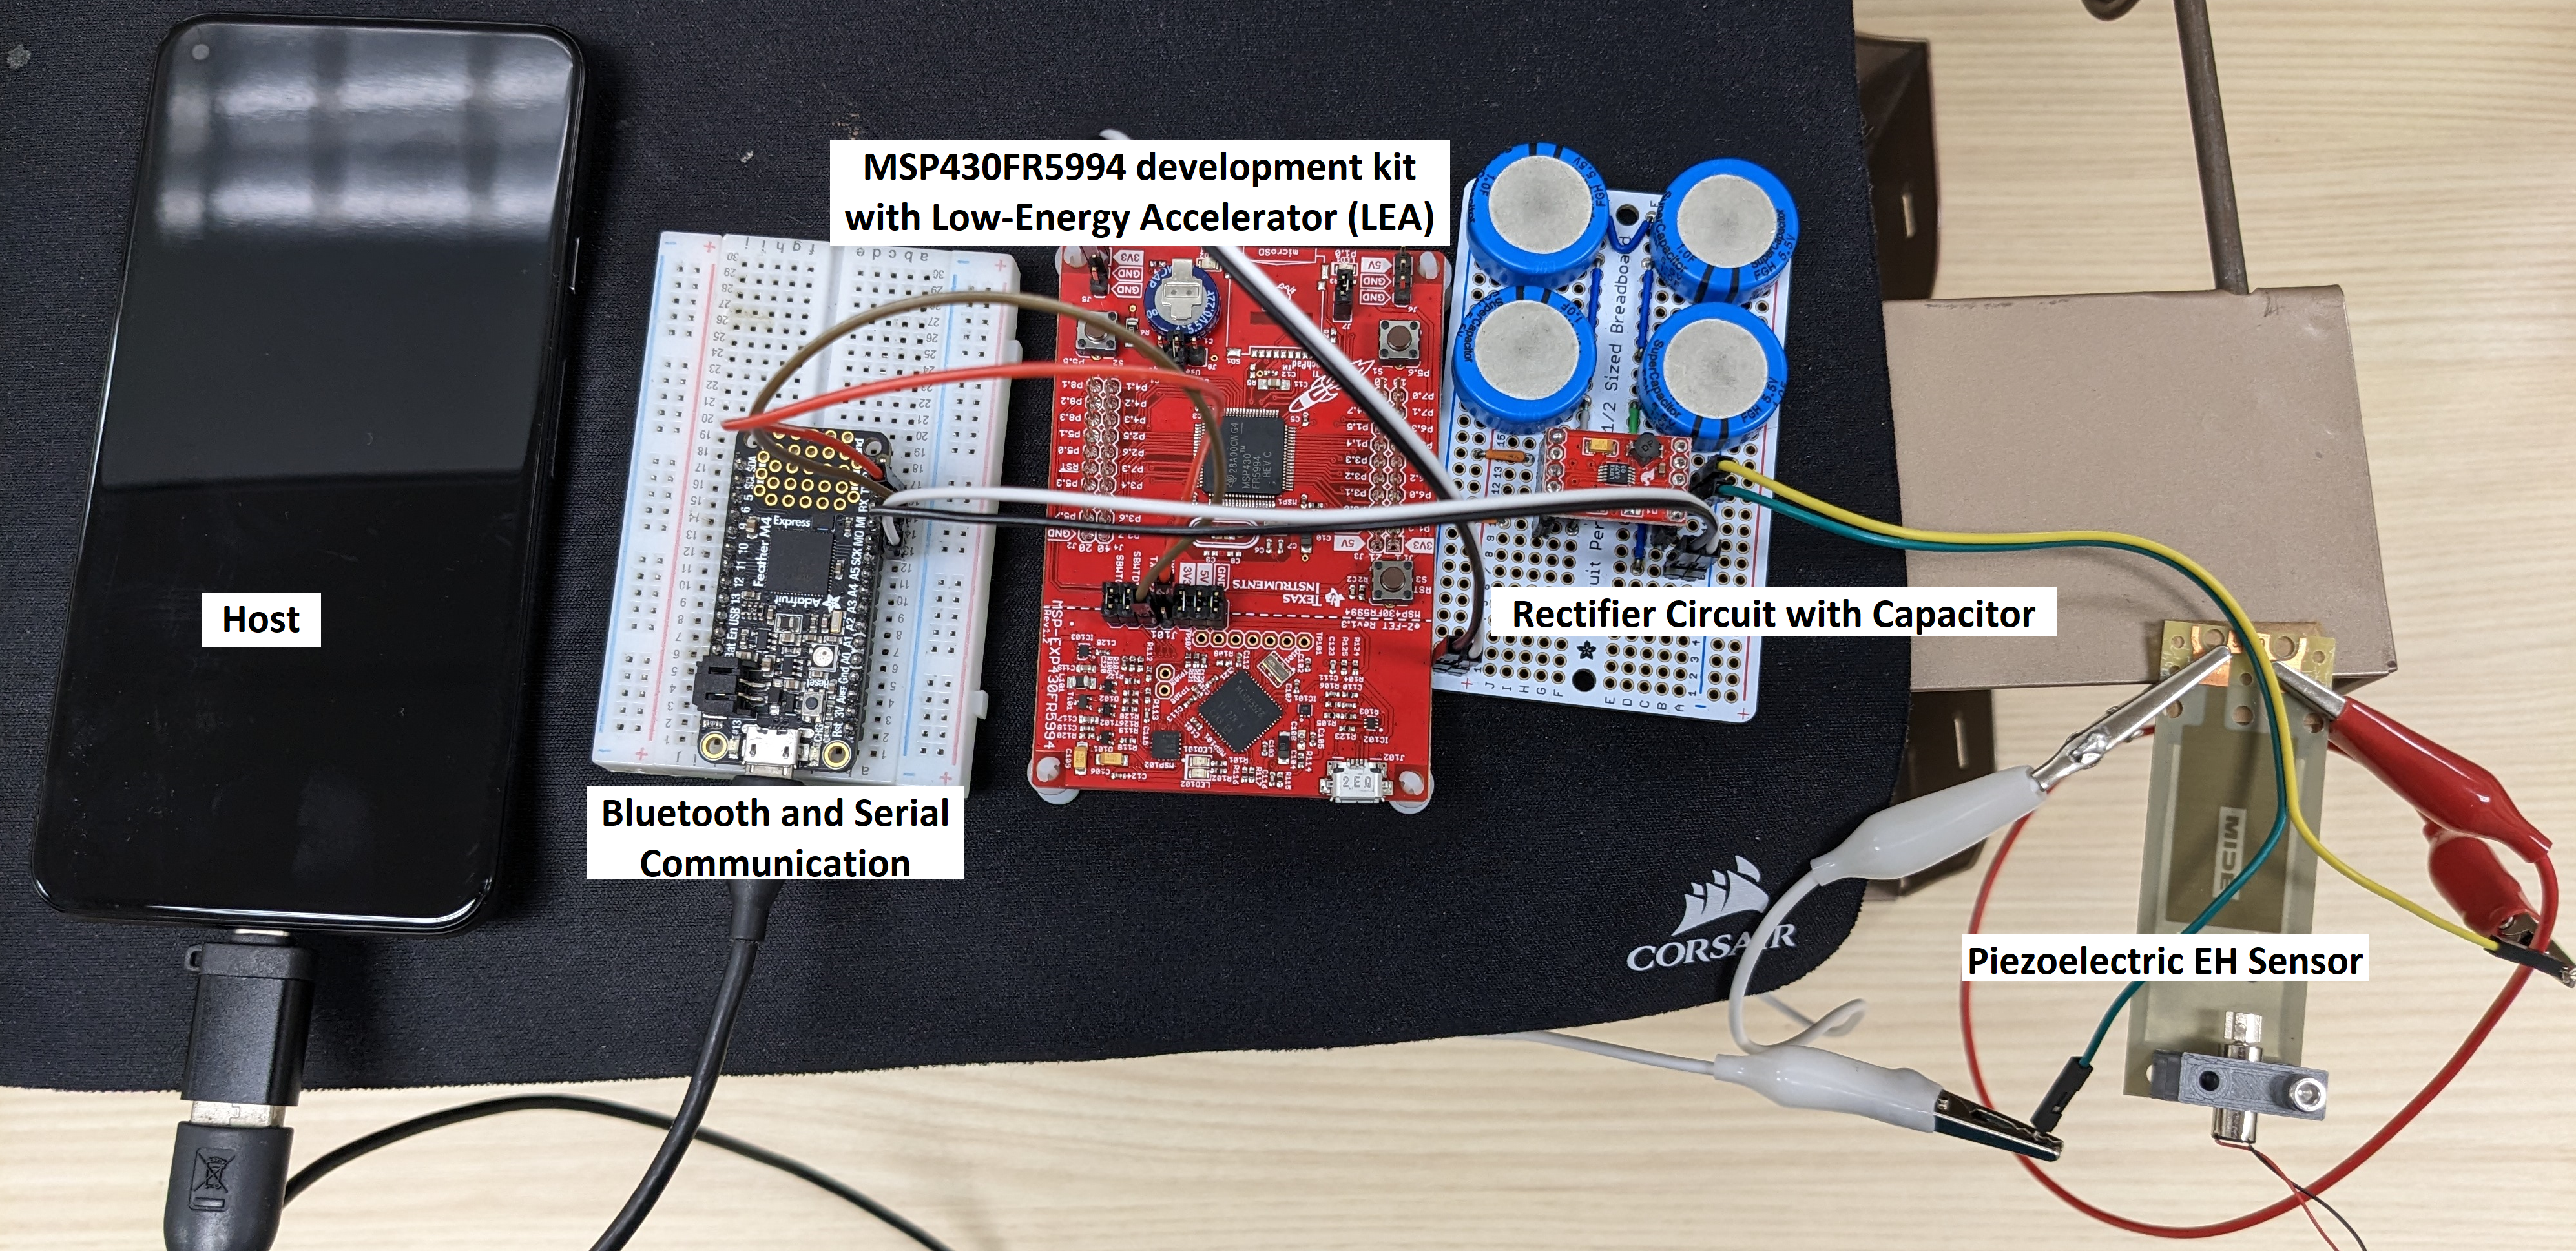
\includegraphics[clip, width=0.5\linewidth]{figs/SeekerCommercial.png}
  \caption{Hardware setup of NExUME using MSP-EXP430FR5994 as the edge compute,   Adafruit ItsyBitsy nRF52840 Express for communicating, Energy Harvester Breakout - LTC3588 with supercapacitors as energy rectification and storage and a Pixel-5 phone as the host.}
  \label{Fig:cotsFIG}
\end{figure}

% Please add the following required packages to your document preamble:
% \usepackage{multirow}
% \usepackage{graphicx}
\begin{table}[H]
\resizebox{\columnwidth}{!}{%
\begin{tabular}{lllllll}
\multicolumn{1}{c}{\multirow{2}{*}{\textbf{Datasets}}} &
  \multicolumn{1}{c}{\multirow{2}{*}{\textbf{Full Power}}} &
  \multicolumn{4}{c}{\textbf{MSP on Piezo}} &
  \textbf{} \\
\multicolumn{1}{c}{} &
  \multicolumn{1}{c}{} &
  \multicolumn{1}{c}{\textbf{AP}} &
  \multicolumn{1}{c}{\textbf{PT}} &
  \multicolumn{1}{c}{\textbf{iNAS+PT}} &
  \multicolumn{1}{c}{\textbf{NExUME}} &
  \textbf{Better} \\
\textbf{FMNIST}     & 98.70 & 71.90 & 79.72 & 83.68 & \textbf{88.90} & 6.24\%  \\
\textbf{CIFAR10}    & 89.81 & 55.05 & 62.00 & 66.98 & \textbf{76.29} & 13.90\% \\
\textbf{MHEALTH}    & 89.62 & 59.76 & 65.40 & 71.56 & \textbf{80.75} & 12.84\% \\
\textbf{PAMAP}      & 87.30 & 57.38 & 65.77 & 65.38 & \textbf{75.16} & 14.97\% \\
\textbf{AudioMNIST} & 88.20 & 67.29 & 73.16 & 75.41 & \textbf{80.01} & 6.10\% 
\end{tabular}%
}
\caption{Accuracy of NExUME on MSP board using vibration from a Piezoelectric harvestor. Better refers to the improvement over iNAS+PT baseline.}
\label{tab:AccMSPonPz}
\end{table}

% Please add the following required packages to your document preamble:
% \usepackage{multirow}
% \usepackage{graphicx}
\begin{table}[H]
\resizebox{\columnwidth}{!}{%
\begin{tabular}{lllllll}
\multicolumn{1}{c}{\multirow{2}{*}{\textbf{Datasets}}} &
  \multicolumn{1}{c}{\multirow{2}{*}{\textbf{Full Power}}} &
  \multicolumn{4}{c}{\textbf{MSP on Thermal}} &
  \textbf{} \\
\multicolumn{1}{c}{} &
  \multicolumn{1}{c}{} &
  \multicolumn{1}{c}{\textbf{AP}} &
  \multicolumn{1}{c}{\textbf{PT}} &
  \multicolumn{1}{c}{\textbf{iNAS+PT}} &
  \multicolumn{1}{c}{\textbf{NExUME}} &
  \textbf{Better} \\
\textbf{FMNIST}     & 98.70 & 80.92 & 86.32 & 88.93 & \textbf{95.62} & 7.53\%  \\
\textbf{CIFAR10}    & 89.81 & 64.78 & 69.29 & 71.53 & \textbf{83.78} & 17.13\% \\
\textbf{MHEALTH}    & 89.62 & 69.77 & 73.99 & 77.70 & \textbf{89.62} & 15.34\% \\
\textbf{PAMAP}      & 87.30 & 66.33 & 71.84 & 74.47 & \textbf{85.24} & 14.46\% \\
\textbf{AudioMNIST} & 88.20 & 73.84 & 78.03 & 81.60 & \textbf{87.64} & 7.40\% 
\end{tabular}%
}
\caption{Accuracy of NExUME on MSP board using thermocouple based thermal harvester. Better refers to the improvement over iNAS+PT baseline.}
\label{tab:AccMSPonTh}
\end{table}

% Please add the following required packages to your document preamble:
% \usepackage{multirow}
% \usepackage{graphicx}
\begin{table}[H]
\resizebox{\columnwidth}{!}{%
\begin{tabular}{lllllll}
\multicolumn{1}{c}{\multirow{2}{*}{\textbf{Datasets}}} &
  \multicolumn{1}{c}{\multirow{2}{*}{\textbf{Full Power}}} &
  \multicolumn{4}{c}{\textbf{Arduino on RF}} &
  \textbf{} \\
\multicolumn{1}{c}{} &
  \multicolumn{1}{c}{} &
  \multicolumn{1}{c}{\textbf{AP}} &
  \multicolumn{1}{c}{\textbf{PT}} &
  \multicolumn{1}{c}{\textbf{iNAS+PT}} &
  \multicolumn{1}{c}{\textbf{NExUME}} &
  \textbf{Better} \\
\textbf{FMNIST}     & 98.70 & 74.44 & 79.63 & 83.61 & \textbf{90.44} & 8.17\%  \\
\textbf{CIFAR10}    & 89.81 & 58.11 & 63.91 & 65.01 & \textbf{79.60} & 22.44\% \\
\textbf{MHEALTH}    & 89.62 & 63.52 & 67.40 & 74.30 & \textbf{83.86} & 12.87\% \\
\textbf{PAMAP}      & 87.30 & 61.39 & 67.24 & 69.45 & \textbf{77.00} & 10.87\% \\
\textbf{AudioMNIST} & 88.20 & 66.11 & 74.28 & 76.60 & \textbf{78.87} & 2.97\% 
\end{tabular}%
}
\caption{Accuracy of NExUME on Arduino nano board using WiFi based RF harvester. Better refers to the improvement over iNAS+PT baseline.}
\label{tab:AccARDonRF}
\end{table}

% Please add the following required packages to your document preamble:
% \usepackage{multirow}
% \usepackage{graphicx}
\begin{table}[H]
\resizebox{\columnwidth}{!}{%
\begin{tabular}{lllllll}
\multicolumn{1}{c}{\multirow{2}{*}{\textbf{Datasets}}} &
  \multicolumn{1}{c}{\multirow{2}{*}{\textbf{Full Power}}} &
  \multicolumn{4}{c}{\textbf{Arduino on Thermal}} &
  \textbf{} \\
\multicolumn{1}{c}{} &
  \multicolumn{1}{c}{} &
  \multicolumn{1}{c}{\textbf{AP}} &
  \multicolumn{1}{c}{\textbf{PT}} &
  \multicolumn{1}{c}{\textbf{iNAS+PT}} &
  \multicolumn{1}{c}{\textbf{NExUME}} &
  \textbf{Better} \\
\textbf{FMNIST}     & 98.70 & 77.04 & 80.44 & 83.08 & \textbf{89.90} & 8.20\%  \\
\textbf{CIFAR10}    & 89.81 & 60.38 & 65.90 & 66.98 & \textbf{80.70} & 20.48\% \\
\textbf{MHEALTH}    & 89.62 & 65.74 & 69.88 & 72.41 & \textbf{85.75} & 18.42\% \\
\textbf{PAMAP}      & 87.30 & 62.76 & 65.93 & 71.46 & \textbf{81.27} & 13.73\% \\
\textbf{AudioMNIST} & 88.20 & 69.12 & 73.86 & 77.79 & \textbf{83.54} & 7.39\% 
\end{tabular}%
}
\caption{Accuracy of NExUME on Arduino nano board using thermocouple based thermal harvester. Better refers to the improvement over iNAS+PT baseline.}
\label{tab:AccARDonTh}
\end{table}


% Please add the following required packages to your document preamble:
% \usepackage{multirow}
% \usepackage{graphicx}


\section{Details on Energy Harvesting}
\label{appendix:EH}
A typical energy harvesting (EH) setup captures and converts environmental energy into usable electrical power, which can then support various electronic devices. Here's a simplified breakdown of the process:

\begin{enumerate}
    \item \textbf{Energy Capture}: The setup begins with a harvester, such as a solar panel, piezoelectric sensor, or thermocouple. These devices are designed to collect energy from their surroundings—light, mechanical vibrations, or heat, respectively.
    \item \textbf{Power Conditioning}: Once energy is harvested, it often needs to be converted and stabilized for use. This is done using a rectifier, which transforms alternating current (AC) into a more usable direct current (DC).
    \item \textbf{Voltage Regulation}: After rectification, the power might not be at the right voltage for the device it needs to support. A matching circuit, including components like buck or boost converters, adjusts the voltage to the appropriate level, ensuring the device receives the correct current and voltage.
    \item \textbf{Energy Storage}: Finally, to ensure a continuous power supply even when the immediate energy source is inconsistent (like when a cloud passes over a solar panel), the system includes a temporary storage unit, such as a super-capacitor. This component helps smooth out the supply, providing steady power to the compute circuit.
\end{enumerate}

By integrating these components, an EH system can sustainably power devices without relying on traditional power grids, making it ideal for remote or mobile applications.

%\sec


\section{Intermittent Computing and Check-pointing}
\label{appendix:ckpt}
\subsection{Intermittency-Aware General Matrix Multiplication (GeMM)}
\label{appendix:intermittentGeMM}
Here we explain the operation of an energy-aware algorithm for performing General Matrix Multiplication (GeMM). The algorithm is designed to operate in environments where energy availability is intermittent, such as in devices powered by energy harvesting. It includes mechanisms for loop tiling, checkpointing, and resumption to manage computation across power interruptions effectively.

\subsubsection{Algorithm Overview}
The GeMM operation, typically expressed as \( C = A \times B \), where \( A \), \( B \), and \( C \) are matrices, is implemented with considerations for energy limitations. The algorithm breaks the matrix multiplication into smaller chunks (tiles), periodically saves the state before potential power losses, and resumes computation from the last saved state upon power restoration.


\subsubsection{Function Definitions}
\begin{itemize}
    \item \textbf{SAVE\_STATE}: Saves the current indices and the partial result of the output matrix \( C \) to non-volatile memory to allow recovery after a power interruption.
    \item \textbf{LOAD\_STATE}: Retrieves the last saved indices and partial result from non-volatile memory to resume computation.
\end{itemize}

\subsubsection{Loop Tiling}
The algorithm uses loop tiling to divide the computation into smaller blocks that can be managed between power interruptions. This tiling not only makes the computation manageable but also optimizes memory usage and cache performance, which is critical in constrained environments.

\subsubsection{Check-pointing Mechanism}
Before each power interruption, detected through an energy monitoring system, the algorithm saves the current state using the \textbf{SAVE\_STATE} function. This state includes the loop indices and the current value of the element being processed in \( C \). This ensures that no computation is lost when the power goes out.

\subsubsection{Resumption Mechanism}
Upon resuming, the algorithm loads the saved state using the \textbf{LOAD\_STATE} function. This state is used to continue the computation exactly where it left off, minimizing redundant operations and ensuring efficiency.


% \subsection{DynInfer with Hardware-Software Support}
% \label{appendix:DynInferFlow}
% We also provide a full software-compiler-hardware driven execution framework for commercial devices with non-volatility support (like MSP-EXP430FR5994 with FeRAM). Figure~\ref{Fig:progflow} shows a detailed overview of our design execution. To support user programs (\ycircled{P1}) we implement a moving window based power predictor (\ycircled{P2}) which takes its input from the on-board EH capacitor. Considering the energy available, the predictor makes an informed decision on how to proceed. The compiler deconstructs the program into \brect{189,215,238}{jobs} to perform seamless program execution. These \brect{189,215,238}{jobs} form the functional program execution DAG. For example, for a DNN execution, the \brect{189,215,238}{jobs} could be CONV2D (\bcircled{C1}), batch normalization (\bcircled{C2}) etc. However, certain \brect{189,215,238}{jobs} could be too big to execute atomically on harvested energy. Therefore, we profile the task using the compute platform (in this case using the MSP-EXP430FR5994 and the LEA in it) to further divide the \brect{189,215,238}{jobs} into \brect{255,192,0}{Power Atomic Tasks} (\brect{255,192,0}{Tasks} hence further). These \brect{255,192,0}{Tasks} are carefully coded with optimized assembly language to maximize their efficiency. We take advantage of \brect{112,173,71}{Hardware Support} (the on-board NV FeRAM) to perform backup and restore in case of \brect{255,0,0}{Power Emergencies}. In case of a power emergency (as shown in Figure~\ref{Fig:progflow} \ccircled{T3}) the task is abandoned and a hardware assisted Backup (\gcircled{Lb}) and Restore (\gcircled{Lr}) is performed. 

% \begin{figure}[H]
%   \centering 
%   \includegraphics[width=0.5\linewidth]{figs/ProgFlow.pdf}
%   \caption{Software-Compiler-Hardware Driven Inference Flow}
%   \label{Fig:progflow}
%   %\vspace{-2pt}
% \end{figure}

% \subsubsection{Algorithmic Steps}
% \begin{algorithm}[H]
\caption{Implementing Depth-wise Separable Convolution - DWSConv2D() using CONV1D()}
\begin{algorithmic}[1]
\Function{DWSepConv2D}{$inputMatrix$, $DWsKernels$, $PtWsKernel$, $outputMatrix$}
    \State Initialize $DWsOutput$ with zero values, same shape as $inputMatrix$
    \State \# Depth-wise Separable (DWs) convolution
    \For{$c \gets 0$ \textbf{to} $channels(inputMatrix) - 1$}
        \State \# Apply 1D convolution along rows
        \For{$i \gets 0$ \textbf{to} $rows(inputMatrix[c]) - 1$}
            \State \Call{conv1D}{$inputMatrix[c][i, :]$, $DWsKernels[c][0, :]$, $DWsOutput[c][i, :]$}
        \EndFor
        \State \# Apply 1D convolution along columns
        \For{$j \gets 0$ \textbf{to} $cols(DWsOutput[c]) - 1$}
            \State \Call{conv1D}{$DWsOutput[c][:, j]$, $DWsKernels[c][:, 0]$, $DWsOutput[c][:, j]$}
        \EndFor
    \EndFor
    \State \# Point-wise (PtWs) convolution
    \State Initialize $finalOutput$ with zero values, with shape [rows($DWsOutput$), cols($DWsOutput$), channels($PtWsKernel$)]
    \For{$i \gets 0$ \textbf{to} $rows(DWsOutput) - 1$}
        \For{$j \gets 0$ \textbf{to} $cols(DWsOutput) - 1$}
            \For{$k \gets 0$ \textbf{to} $channels(PtWsKernel) - 1$}
                \State Initialize $PtWsSum \gets 0$
                \For{$c \gets 0$ \textbf{to} $channels(DWsOutput) - 1$}
                    \State $PtWsSum \gets PtWsSum + DWsOutput[c][i][j] \times PtWsKernel[c][k]$
                \EndFor
                \State $finalOutput[i][j][k] \gets PtWsSum$
            \EndFor
        \EndFor
    \EndFor
    \State \Return $finalOutput$
\EndFunction
\end{algorithmic}
\label{conv1D2conv2D}
\end{algorithm}


% \subsection{Task Completion under Intermittent Execution}
% \label{appendix:complete}

\section{Formulation of Dynamic Dropouts:}
\label{appendix:DynDropMath}
\input{Appendix/L2Dynamic}
\subsection{Optimal Brain Damage Dropout with QuantaTask Optimization}
\label{appendix:obd}
Optimal Brain Damage Dropout leverages a simplified version of the Optimal Brain Damage pruning method to adjust dropout rates, combined with the QuantaTask optimization to handle energy constraints in intermittent systems.

\textbf{Mathematical Formulation:}
Let \(\mathbf{W}\) be the weight matrix of a layer. The sensitivity of each weight \(W_{ij}\) is calculated using the second-order Taylor expansion of the loss function \(\mathcal{L}\):
\[
\Delta \mathcal{L} \approx \frac{1}{2} \sum_{i,j} \frac{\partial^2 \mathcal{L}}{\partial W_{ij}^2} (W_{ij})^2
\]
where \(\frac{\partial^2 \mathcal{L}}{\partial W_{ij}^2}\) is the second-order derivative (Hessian) of the loss with respect to the weights.

Define the dropout probability \(p_i\) for neuron \(i\) based on the sensitivity of its corresponding weights. The idea is to use the sensitivity to determine the probability:
\[
p_i = \frac{\beta \sum_j \frac{\partial^2 \mathcal{L}}{\partial W_{ij}^2} (W_{ij})^2}{\max \left( \sum_j \frac{\partial^2 \mathcal{L}}{\partial W_{ij}^2} (W_{ij})^2 \right) + \epsilon}
\]
where \(\beta\) is a scaling factor to adjust the overall dropout rate, and \(\epsilon\) is a small constant to avoid division by zero.

Define a binary dropout mask \(\mathbf{m} = [m_1, m_2, \ldots, m_n]\) where \(m_i \in \{0, 1\}\). Each element of the mask is determined by sampling from a Bernoulli distribution with probability \(1 - p_i\):
\[
m_i \sim \text{Bernoulli}(1 - p_i)
\]

Apply the dropout mask during the forward pass. Let \(\mathbf{a}_i\) denote the activation of neuron \(i\):
\[
\mathbf{a}_i^{\text{dropout}} = \mathbf{a}_i \cdot m_i
\]


\textbf{Training with Optimal Brain Damage Dropout and QuantaTask Optimization:}
Initialize the network parameters \(\mathbf{W}\), dropout mask \(\mathbf{m}\), and scaling factor \(\beta\). Define the energy budget \(E_b\) for a single quanta and for the entire inference. Initialize the loop iteration parameters \(l\).


Compute the activations \(\mathbf{a}\) and apply the dropout mask:
\[
\mathbf{a}_i^{\text{dropout}} = \mathbf{a}_i \cdot m_i
\]

Compute the loss \(\mathcal{L}(\mathbf{Y}, \mathbf{\hat{Y}})\) where \(\mathbf{Y}\) is the output of the network and \(\mathbf{\hat{Y}}\) is the target output.

Calculate the gradients and Hessians of the loss with respect to the weights:
\[
\frac{\partial \mathcal{L}}{\partial W_{ij}}, \quad \frac{\partial^2 \mathcal{L}}{\partial W_{ij}^2}
\]

For each layer \(L\) and loop \(i\) within the layer, estimate the energy \(E_i\) required for the current quanta size \(l_i\):
\[
E_i \gets \text{DynAgent.estimateEnergy}(L, i, l_i)
\]
If \(E_i > E_b\), fuse tasks to reduce the overhead:
\[
\text{FuseTasks}(L, i, l_i, E_b)
\]
Update \(E_i\) after task fusion:
\[
E_i \gets \text{DynAgent.estimateEnergy}(L, i, l_i)
\]

Update the dropout mask \(\mathbf{m}\) based on the sensitivities:
\[
p_i = \frac{\beta \sum_j \frac{\partial^2 \mathcal{L}}{\partial W_{ij}^2} (W_{ij})^2}{\max \left( \sum_j \frac{\partial^2 \mathcal{L}}{\partial W_{ij}^2} (W_{ij})^2 \right) + \epsilon}
\]
\[
m_i = 
\begin{cases} 
0 & \text{if } \text{Bernoulli}(1 - p_i) = 0 \\
1 & \text{otherwise}
\end{cases}
\]

Perform the backward pass to update the network weights, considering the dropout mask:
\[
\mathbf{W} \leftarrow \mathbf{W} - \eta \frac{\partial \mathcal{L}}{\partial \mathbf{W}} \odot \mathbf{m}
\]
where \(\eta\) is the learning rate and \(\odot\) denotes element-wise multiplication.

\textbf{Inference with Optimal Brain Damage Dropout and QuantaTask Optimization:}
Check the available energy using DynAgent.
If energy is below a threshold, increase the dropout rate to ensure the inference can be completed within the energy budget. Otherwise, maintain or reduce the dropout rate to improve accuracy.
Perform the forward pass with the updated dropout mask to obtain the output \(\mathbf{Y}\).
This approach ensures that the network is robust to varying energy conditions by incorporating dynamic dropout influenced by the sensitivity of the weights, along with the QuantaTask optimization to handle energy constraints.

\subsection{Feature Map Reconstruction Error Dropout with QuantaTask Optimization}
\label{appendix:FMRE}
Feature Map Reconstruction Error Dropout leverages the reconstruction error of feature maps to adjust dropout rates, combined with the QuantaTask optimization to handle energy constraints in intermittent systems.

\textbf{Mathematical Formulation:}
Let \(\mathbf{W}\) be the weight matrix of a layer and \(\mathbf{F}\) be the feature maps produced by the layer. The reconstruction error of a feature map \(F_i\) is calculated as:
\[
\text{RE}_i = \|\mathbf{F}_i - \hat{\mathbf{F}}_i\|_2
\]
where \(\hat{\mathbf{F}}_i\) is the reconstructed feature map, and \(\|\cdot\|_2\) denotes the L2 norm.

Define the dropout probability \(p_i\) for neuron \(i\) based on the reconstruction error of its corresponding feature map. The idea is to use the reconstruction error to determine the probability:
\[
p_i = \frac{\gamma \, \text{RE}_i}{\max(\text{RE}) + \epsilon}
\]
where \(\gamma\) is a scaling factor to adjust the overall dropout rate, and \(\epsilon\) is a small constant to avoid division by zero.

Define a binary dropout mask \(\mathbf{m} = [m_1, m_2, \ldots, m_n]\) where \(m_i \in \{0, 1\}\). Each element of the mask is determined by sampling from a Bernoulli distribution with probability \(1 - p_i\):
\[
m_i \sim \text{Bernoulli}(1 - p_i)
\]

Apply the dropout mask during the forward pass. Let \(\mathbf{a}_i\) denote the activation of neuron \(i\):
\[
\mathbf{a}_i^{\text{dropout}} = \mathbf{a}_i \cdot m_i
\]

\textbf{Training with Feature Map Reconstruction Error Dropout and QuantaTask Optimization:}
Initialize the network parameters \(\mathbf{W}\), dropout mask \(\mathbf{m}\), and scaling factor \(\gamma\). Define the energy budget \(E_b\) for a single quanta and for the entire inference. Initialize the loop iteration parameters \(l\).


Compute the activations \(\mathbf{a}\) and apply the dropout mask:
\[
\mathbf{a}_i^{\text{dropout}} = \mathbf{a}_i \cdot m_i
\]

Compute the loss \(\mathcal{L}(\mathbf{Y}, \mathbf{\hat{Y}})\) where \(\mathbf{Y}\) is the output of the network and \(\mathbf{\hat{Y}}\) is the target output.

Calculate the gradients of the loss with respect to the weights:
\[
\frac{\partial \mathcal{L}}{\partial W_{ij}}
\]

For each layer \(L\) and loop \(i\) within the layer, estimate the energy \(E_i\) required for the current quanta size \(l_i\):
\[
E_i \gets \text{DynAgent.estimateEnergy}(L, i, l_i)
\]
If \(E_i > E_b\), fuse tasks to reduce the overhead:
\[
\text{FuseTasks}(L, i, l_i, E_b)
\]
Update \(E_i\) after task fusion:
\[
E_i \gets \text{DynAgent.estimateEnergy}(L, i, l_i)
\]

Update the dropout mask \(\mathbf{m}\) based on the reconstruction error of the feature maps:
\[
p_i = \frac{\gamma \, \text{RE}_i}{\max(\text{RE}) + \epsilon}
\]
\[
m_i = 
\begin{cases} 
0 & \text{if } \text{Bernoulli}(1 - p_i) = 0 \\
1 & \text{otherwise}
\end{cases}
\]

Perform the backward pass to update the network weights, considering the dropout mask:
\[
\mathbf{W} \leftarrow \mathbf{W} - \eta \frac{\partial \mathcal{L}}{\partial \mathbf{W}} \odot \mathbf{m}
\]
where \(\eta\) is the learning rate and \(\odot\) denotes element-wise multiplication.

\textbf{Inference with Feature Map Reconstruction Error Dropout and QuantaTask Optimization:}
Check the available energy using DynAgent.
If energy is below a threshold, increase the dropout rate to ensure the inference can be completed within the energy budget. Otherwise, maintain or reduce the dropout rate to improve accuracy.
Perform the forward pass with the updated dropout mask to obtain the output \(\mathbf{Y}\).
This approach ensures that the network is robust to varying energy conditions by incorporating dynamic dropout influenced by the reconstruction error of the feature maps, along with the QuantaTask optimization to handle energy constraints.
\subsection{Learning Sparse Masks Dropout with QuantaTask Optimization}
\label{appendix:spmask}
Learning Sparse Masks Dropout adapts dropout masks as learnable parameters within the network, inspired by Wen et al. (2016), combined with the QuantaTask optimization to handle energy constraints in intermittent systems.

\textbf{Mathematical Formulation:}
Let \(\mathbf{W}\) be the weight matrix of a layer. Define a binary dropout mask \(\mathbf{m} = [m_1, m_2, \ldots, m_n]\) where \(m_i \in \{0, 1\}\). In Learning Sparse Masks Dropout, the dropout masks are treated as learnable parameters. The mask values are determined using a sigmoid function to ensure they lie between 0 and 1:
\[
m_i = \sigma(z_i)
\]
where \(z_i\) are learnable parameters and \(\sigma(\cdot)\) is the sigmoid function.

Apply the dropout mask during the forward pass. Let \(\mathbf{a}_i\) denote the activation of neuron \(i\):
\[
\mathbf{a}_i^{\text{dropout}} = \mathbf{a}_i \cdot m_i
\]

Compute the loss \(\mathcal{L}(\mathbf{Y}, \mathbf{\hat{Y}})\) where \(\mathbf{Y}\) is the output of the network and \(\mathbf{\hat{Y}}\) is the target output.

DynFit integrates closely with DynAgent, which serves as a repository of EH profiles and hardware characteristics. Let \(\mathcal{Q}\) represent the set of execution quanta, where each quanta \(q \in \mathcal{Q}\) is defined by a tuple \((l, e)\):
\[
q = (l, e)
\]
Here, \(l\) is the number of loop iterations and \(e\) is the estimated energy required for these iterations. The goal is to optimize the loop iteration parameter \(l\) such that the energy consumption \(E_q\) for each quanta \(q\) is within the energy budget \(E_b\):
\[
\text{minimize} \quad \sum_{q \in \mathcal{Q}} E_q \quad \text{subject to} \quad E_q \leq E_b
\]

\textbf{Training with Learning Sparse Masks Dropout and QuantaTask Optimization:}
Initialize the network parameters \(\mathbf{W}\), dropout mask parameters \(\mathbf{z}\), and scaling factor \(\alpha\). Define the energy budget \(E_b\) for a single quanta and for the entire inference. Initialize the loop iteration parameters \(l\).

Compute the activations \(\mathbf{a}\) and apply the dropout mask:
\[
m_i = \sigma(z_i)
\]
\[
\mathbf{a}_i^{\text{dropout}} = \mathbf{a}_i \cdot m_i
\]

Compute the loss \(\mathcal{L}(\mathbf{Y}, \mathbf{\hat{Y}})\). Calculate the gradients of the loss with respect to the weights and dropout mask parameters:
\[
\frac{\partial \mathcal{L}}{\partial W_{ij}}, \quad \frac{\partial \mathcal{L}}{\partial z_i}
\]
For each layer \(L\) and loop \(i\) within the layer, estimate the energy \(E_i\) required for the current quanta size \(l_i\):
\[
E_i \gets \text{DynAgent.estimateEnergy}(L, i, l_i)
\]
If \(E_i > E_b\), fuse tasks to reduce the overhead:
\[
\text{FuseTasks}(L, i, l_i, E_b)
\]
Update \(E_i\) after task fusion:
\[
E_i \gets \text{DynAgent.estimateEnergy}(L, i, l_i)
\]


Update the dropout mask parameters \(\mathbf{z}\) based on the gradients:
\[
z_i \leftarrow z_i - \eta \frac{\partial \mathcal{L}}{\partial z_i}
\]

Perform the backward pass to update the network weights, considering the dropout mask:
\[
\mathbf{W} \leftarrow \mathbf{W} - \eta \frac{\partial \mathcal{L}}{\partial \mathbf{W}} \odot \mathbf{m}
\]
where \(\eta\) is the learning rate and \(\odot\) denotes element-wise multiplication.

\textbf{Inference with Learning Sparse Masks Dropout and QuantaTask Optimization:}
Check the available energy using DynAgent.
If energy is below a threshold, increase the dropout rate to ensure the inference can be completed within the energy budget. Otherwise, maintain or reduce the dropout rate to improve accuracy.
Perform the forward pass with the updated dropout mask to obtain the output \(\mathbf{Y}\).
This approach ensures that the network is robust to varying energy conditions by incorporating dynamic dropout with learnable mask parameters, along with the QuantaTask optimization to handle energy constraints.
\subsection{Neuron Shapley Value Dropout with QuantaTask Optimization}
\label{appendix:shapely}
Neuron Shapley Value Dropout applies the concept of Shapley values from game theory (Aas et al., 2021) to assess neuron importance for dropout, combined with the QuantaTask optimization to handle energy constraints in intermittent systems.

\textbf{Mathematical Formulation:}
The Shapley value \(\phi_i\) of neuron \(i\) is a measure of its contribution to the overall network performance. It is calculated by considering all possible subsets of neurons and computing the marginal contribution of neuron \(i\) to the network's output:
\[
\phi_i = \frac{1}{|\mathcal{N}|!} \sum_{S \subseteq \mathcal{N} \setminus \{i\}} \frac{|S|! (|\mathcal{N}| - |S| - 1)!}{|\mathcal{N}|} \left[ \mathcal{L}(S \cup \{i\}) - \mathcal{L}(S) \right]
\]
where \(\mathcal{N}\) is the set of all neurons, \(S\) is a subset of neurons not containing \(i\), and \(\mathcal{L}(\cdot)\) denotes the loss function.

Define the dropout probability \(p_i\) for neuron \(i\) based on its Shapley value. Neurons with lower Shapley values are more likely to be dropped:
\[
p_i = \frac{\delta}{\phi_i + \epsilon}
\]
where \(\delta\) is a scaling factor to adjust the overall dropout rate, and \(\epsilon\) is a small constant to avoid division by zero.

Define a binary dropout mask \(\mathbf{m} = [m_1, m_2, \ldots, m_n]\) where \(m_i \in \{0, 1\}\). Each element of the mask is determined by sampling from a Bernoulli distribution with probability \(1 - p_i\):
\[
m_i \sim \text{Bernoulli}(1 - p_i)
\]

Apply the dropout mask during the forward pass. Let \(\mathbf{a}_i\) denote the activation of neuron \(i\):
\[
\mathbf{a}_i^{\text{dropout}} = \mathbf{a}_i \cdot m_i
\]

\textbf{Training with Neuron Shapley Value Dropout and QuantaTask Optimization:}
Initialize the network parameters \(\mathbf{W}\), dropout mask \(\mathbf{m}\), and scaling factor \(\delta\). Define the energy budget \(E_b\) for a single quanta and for the entire inference. Initialize the loop iteration parameters \(l\).

Compute the activations \(\mathbf{a}\) and apply the dropout mask:
\[
\mathbf{a}_i^{\text{dropout}} = \mathbf{a}_i \cdot m_i
\]

Compute the loss \(\mathcal{L}(\mathbf{Y}, \mathbf{\hat{Y}})\) where \(\mathbf{Y}\) is the output of the network and \(\mathbf{\hat{Y}}\) is the target output.

Calculate the Shapley values \(\phi_i\) for each neuron based on their contribution to the network's performance.

For each layer \(L\) and loop \(i\) within the layer, estimate the energy \(E_i\) required for the current quanta size \(l_i\):
\[
E_i \gets \text{DynAgent.estimateEnergy}(L, i, l_i)
\]
If \(E_i > E_b\), fuse tasks to reduce the overhead:
\[
\text{FuseTasks}(L, i, l_i, E_b)
\]
Update \(E_i\) after task fusion:
\[
E_i \gets \text{DynAgent.estimateEnergy}(L, i, l_i)
\]

Update the dropout mask \(\mathbf{m}\) based on the Shapley values:
\[
p_i = \frac{\delta}{\phi_i + \epsilon}
\]
\[
m_i = 
\begin{cases} 
0 & \text{if } \text{Bernoulli}(1 - p_i) = 0 \\
1 & \text{otherwise}
\end{cases}
\]

Perform the backward pass to update the network weights, considering the dropout mask:
\[
\mathbf{W} \leftarrow \mathbf{W} - \eta \frac{\partial \mathcal{L}}{\partial \mathbf{W}} \odot \mathbf{m}
\]
where \(\eta\) is the learning rate and \(\odot\) denotes element-wise multiplication.

\textbf{Inference with Neuron Shapley Value Dropout and QuantaTask Optimization:}
Check the available energy using DynAgent.
If energy is below a threshold, increase the dropout rate to ensure the inference can be completed within the energy budget. Otherwise, maintain or reduce the dropout rate to improve accuracy.
Perform the forward pass with the updated dropout mask to obtain the output \(\mathbf{Y}\).
This approach ensures that the network is robust to varying energy conditions by incorporating dynamic dropout influenced by the Shapley values of the neurons, along with the QuantaTask optimization to handle energy constraints.

\subsection{Taylor Expansion Dropout with QuantaTask Optimization}
\label{appendix:taylor}
Taylor Expansion Dropout uses Taylor expansion (Li et al., 2016) to evaluate the impact of neurons on loss for dropout adjustments, combined with the QuantaTask optimization to handle energy constraints in intermittent systems.

\textbf{Mathematical Formulation:}
Let \(\mathbf{W}\) be the weight matrix of a layer. The impact of neuron \(i\) on the loss function \(\mathcal{L}\) can be approximated using the first-order Taylor expansion:
\[
\Delta \mathcal{L}_i \approx \left| \frac{\partial \mathcal{L}}{\partial \mathbf{a}_i} \mathbf{a}_i \right|
\]
where \(\mathbf{a}_i\) is the activation of neuron \(i\), and \(\frac{\partial \mathcal{L}}{\partial \mathbf{a}_i}\) is the gradient of the loss with respect to the activation.

Define the dropout probability \(p_i\) for neuron \(i\) based on the Taylor expansion approximation of its impact on the loss:
\[
p_i = \frac{\lambda}{\left| \frac{\partial \mathcal{L}}{\partial \mathbf{a}_i} \mathbf{a}_i \right| + \epsilon}
\]
where \(\lambda\) is a scaling factor to adjust the overall dropout rate, and \(\epsilon\) is a small constant to avoid division by zero.

Define a binary dropout mask \(\mathbf{m} = [m_1, m_2, \ldots, m_n]\) where \(m_i \in \{0, 1\}\). Each element of the mask is determined by sampling from a Bernoulli distribution with probability \(1 - p_i\):
\[
m_i \sim \text{Bernoulli}(1 - p_i)
\]

Apply the dropout mask during the forward pass. Let \(\mathbf{a}_i\) denote the activation of neuron \(i\):
\[
\mathbf{a}_i^{\text{dropout}} = \mathbf{a}_i \cdot m_i
\]

\textbf{Training with Taylor Expansion Dropout and QuantaTask Optimization:}
Initialize the network parameters \(\mathbf{W}\), dropout mask \(\mathbf{m}\), and scaling factor \(\lambda\). Define the energy budget \(E_b\) for a single quanta and for the entire inference. Initialize the loop iteration parameters \(l\).

Compute the activations \(\mathbf{a}\) and apply the dropout mask:
\[
\mathbf{a}_i^{\text{dropout}} = \mathbf{a}_i \cdot m_i
\]

Compute the loss \(\mathcal{L}(\mathbf{Y}, \mathbf{\hat{Y}})\) where \(\mathbf{Y}\) is the output of the network and \(\mathbf{\hat{Y}}\) is the target output.

Calculate the gradients of the loss with respect to the activations:
\[
\frac{\partial \mathcal{L}}{\partial \mathbf{a}_i}
\]

For each layer \(L\) and loop \(i\) within the layer, estimate the energy \(E_i\) required for the current quanta size \(l_i\):
\[
E_i \gets \text{DynAgent.estimateEnergy}(L, i, l_i)
\]
If \(E_i > E_b\), fuse tasks to reduce the overhead:
\[
\text{FuseTasks}(L, i, l_i, E_b)
\]
Update \(E_i\) after task fusion:
\[
E_i \gets \text{DynAgent.estimateEnergy}(L, i, l_i)
\]

Update the dropout mask \(\mathbf{m}\) based on the Taylor expansion approximation:
\[
p_i = \frac{\lambda}{\left| \frac{\partial \mathcal{L}}{\partial \mathbf{a}_i} \mathbf{a}_i \right| + \epsilon}
\]
\[
m_i = 
\begin{cases} 
0 & \text{if } \text{Bernoulli}(1 - p_i) = 0 \\
1 & \text{otherwise}
\end{cases}
\]

Perform the backward pass to update the network weights, considering the dropout mask:
\[
\mathbf{W} \leftarrow \mathbf{W} - \eta \frac{\partial \mathcal{L}}{\partial \mathbf{W}} \odot \mathbf{m}
\]
where \(\eta\) is the learning rate and \(\odot\) denotes element-wise multiplication.

\textbf{Inference with Taylor Expansion Dropout and QuantaTask Optimization:}
Check the available energy using DynAgent.
If energy is below a threshold, increase the dropout rate to ensure the inference can be completed within the energy budget. Otherwise, maintain or reduce the dropout rate to improve accuracy.
Perform the forward pass with the updated dropout mask to obtain the output \(\mathbf{Y}\).
This approach ensures that the network is robust to varying energy conditions by incorporating dynamic dropout influenced by the Taylor expansion approximation of the neurons' impact on the loss, along with the QuantaTask optimization to handle energy constraints.

% \section{Pseudo Codes}
% \label{appendix:LEAcodes}
% \subsection{Depth-wise Separable Convolution 2D Using TI LEA}
Depth-wise separable convolution is an efficient form of convolution that reduces the computational cost compared to standard convolution. Here we describe the implementation of depth-wise separable convolution 2D using the Low Energy Accelerator (LEA) in Texas Instruments' MSP430 microcontrollers.

\subsubsection{depth-wise Separable Convolution 2D Using Conv1D}
\label{appendix:pDWSC}
%%%%%
The pseudo code described in Algorithm~\ref{algo:conv1D2conv2D-here} implements a depth-wise separable convolution 2D (DWSConv2D) using a 1D convolution primitive function (conv1D). The DWSConv2D function takes four inputs: an input matrix, depth-wise kernels (DWsKernels), point-wise kernels (PtWsKernel), and an output matrix. The depth-wise separable convolution is performed in two main steps: depth-wise convolution and point-wise convolution.
%\begin{algorithm}[H]
\label{algo:conv1D2conv2D}
\caption{Implementing Depth-wise Separable Convolution - DWSConv2D() using CONV1D ()}
\begin{algorithmic}[1]
\State \textbf{Function} DWSepConv2D($inputMatrix$, $DWsKernels$, $PtWsKernel$, $outputMatrix$):
\State \quad Initialize $DWsOutput$ with zero values, same shape as $inputMatrix$
\State \quad \# Depth-wise Separable (DWs) convolution
\State \quad \textbf{for} $c \leftarrow 0$ \textbf{to} $channels(inputMatrix) - 1$:
\State \quad \quad \# Apply 1D convolution along rows
\State \quad \quad \textbf{for} $i \leftarrow 0$ \textbf{to} $rows(inputMatrix[c]) - 1$:
\State \quad \quad \quad conv1D($inputMatrix[c][i, :]$, $DWsKernels[c][0, :]$, $DWsOutput[c][i, :]$)
\State \quad \quad \# Apply 1D convolution along columns
\State \quad \quad \textbf{for} $j \leftarrow 0$ \textbf{to} $cols(DWsOutput[c]) - 1$:
\State \quad \quad \quad conv1D($DWsOutput[c][:, j]$, $DWsKernels[c][:, 0]$, $DWsOutput[c][:, j]$)
\State \quad \# Point-wise (PtWs) convolution
\State \quad Initialize $finalOutput$ with zero values, with shape [rows($DWsOutput$), cols($DWsOutput$), channels($PtWsKernel$)]
\State \quad \textbf{for} $i \leftarrow 0$ \textbf{to} $rows(DWsOutput) - 1$:
\State \quad \quad \textbf{for} $j \leftarrow 0$ \textbf{to} $cols(DWsOutput) - 1$:
\State \quad \quad \quad \textbf{for} $k \leftarrow 0$ \textbf{to} $channels(PtWsKernel) - 1$:
\State \quad \quad \quad \quad Initialize $PtWsSum \leftarrow 0$
\State \quad \quad \quad \quad \textbf{for} $c \leftarrow 0$ \textbf{to} $channels(DWsOutput) - 1$:
\State \quad \quad \quad \quad \quad $PtWsSum \leftarrow PtWsSum + DWsOutput[c][i][j] \times PtWsKernel[c][k]$
\State \quad \quad \quad \quad $finalOutput[i][j][k] \leftarrow PtWsSum$
\State \quad \textbf{return} $finalOutput$
\end{algorithmic}
\end{algorithm}
\begin{algorithm}[H]
\caption{Implementing Depth-wise Separable Convolution - DWSConv2D() using CONV1D ()}
\begin{algorithmic}[1]
\State \textbf{Function} DWSepConv2D($inputMatrix$, $DWsKernels$, $PtWsKernel$, $outputMatrix$):
\State \quad Initialize $DWsOutput$ with zero values, same shape as $inputMatrix$
\State \quad \# Depth-wise Separable (DWs) convolution
\State \quad \textbf{for} $c \leftarrow 0$ \textbf{to} $channels(inputMatrix) - 1$:
\State \quad \quad \# Apply 1D convolution along rows
\State \quad \quad \textbf{for} $i \leftarrow 0$ \textbf{to} $rows(inputMatrix[c]) - 1$:
\State \quad \quad \quad conv1D($inputMatrix[c][i, :]$, $DWsKernels[c][0, :]$, $DWsOutput[c][i, :]$)
\State \quad \quad \# Apply 1D convolution along columns
\State \quad \quad \textbf{for} $j \leftarrow 0$ \textbf{to} $cols(DWsOutput[c]) - 1$:
\State \quad \quad \quad conv1D($DWsOutput[c][:, j]$, $DWsKernels[c][:, 0]$, $DWsOutput[c][:, j]$)
\State \quad \# Point-wise (PtWs) convolution
\State \quad Initialize $finalOutput$ with zero values, with shape [rows($DWsOutput$), cols($DWsOutput$), channels($PtWsKernel$)]
\State \quad \textbf{for} $i \leftarrow 0$ \textbf{to} $rows(DWsOutput) - 1$:
\State \quad \quad \textbf{for} $j \leftarrow 0$ \textbf{to} $cols(DWsOutput) - 1$:
\State \quad \quad \quad \textbf{for} $k \leftarrow 0$ \textbf{to} $channels(PtWsKernel) - 1$:
\State \quad \quad \quad \quad Initialize $PtWsSum \leftarrow 0$
\State \quad \quad \quad \quad \textbf{for} $c \leftarrow 0$ \textbf{to} $channels(DWsOutput) - 1$:
\State \quad \quad \quad \quad \quad $PtWsSum \leftarrow PtWsSum + DWsOutput[c][i][j] \times PtWsKernel[c][k]$
\State \quad \quad \quad \quad $finalOutput[i][j][k] \leftarrow PtWsSum$
\State \quad \textbf{return} $finalOutput$
\end{algorithmic}
\label{algo:conv1D2conv2D-here}
\end{algorithm}


% {\textbf{Explanation}}

% {Step 1: Depth-wise Separable (DWs) Convolution}

% The first step in the DWSConv2D function is to perform depth-wise separable convolution. This process involves applying 1D convolution along both the rows and columns of each channel in the input matrix. The depth-wise convolution is done separately for each channel using its corresponding filter in the DWsKernels.

% \begin{itemize}
%     \item \textbf{Initialize DWsOutput}: A matrix of zeros with the same shape as the input matrix.
%     \item \textbf{Loop over channels}: For each channel in the input matrix:
%     \begin{itemize}
%         \item \textbf{1D Convolution along Rows}: For each row in the channel, apply the 1D convolution using the conv1D function with the corresponding row filter from DWsKernels.
%         \item \textbf{1D Convolution along Columns}: For each column in the DWsOutput channel, apply the 1D convolution using the conv1D function with the corresponding column filter from DWsKernels.
%     \end{itemize}
% \end{itemize}

% {Step 2: Point-wise (PtWs) Convolution}

% The second step is to perform point-wise convolution on the depth-wise convolved output (DWsOutput). This involves applying the PtWsKernel to each spatial position in the DWsOutput across all channels.

% \begin{itemize}
%     \item \textbf{Initialize finalOutput}: A matrix of zeros with the shape [rows(DWsOutput), cols(DWsOutput), channels(PtWsKernel)].
%     \item \textbf{Loop over spatial positions} ($i$, $j$): For each spatial position in DWsOutput:
%     \begin{itemize}
%         \item \textbf{Loop over point-wise filters} ($k$): For each filter in PtWsKernel:
%         \begin{itemize}
%             \item Initialize $PtWsSum$ to zero.
%             \item \textbf{Accumulate the point-wise sum}: For each channel in DWsOutput, multiply the value at the spatial position by the corresponding value in PtWsKernel and add to $PtWsSum$.
%             \item Assign $PtWsSum$ to the corresponding position in finalOutput.
%         \end{itemize}
%     \end{itemize}
% \end{itemize}

% The function finally returns the result stored in $finalOutput$.


%%%%%%


\subsubsection{Pseudocode with micro-controller primitives}
\label{appendix:leaDWSC}
The following pseudocode describes the steps to implement depth-wise separable convolution using LEA primitives from TI's DSP Library.

\begin{algorithm}[H]
\caption{depth-wise Separable Convolution 2D Using TI LEA}
\begin{algorithmic}[1]
\Function{DWSepConv2D}{$inputMatrix$, $DWsKernels$, $PtWsKernel$, $outputMatrix$}
    \State Initialize $tempMatrix1$ and $tempMatrix2$ with zero values, same shape as $inputMatrix$
    \State // Depth-wise convolution
    \For{$c \gets 0$ \textbf{to} $channels(inputMatrix) - 1$}
        \State // Apply 1D convolution along rows
        \For{$i \gets 0$ \textbf{to} $rows(inputMatrix[c]) - 1$}
            \State \Call{msp\_conv\_iq31}{$inputMatrix[c][i, :]$, $DWsKernels[c][0, :]$, $tempMatrix1[c][i, :]$, $cols(inputMatrix)$, $FILTER\_SIZE$}
        \EndFor
        \State // Apply 1D convolution along columns
        \For{$j \gets 0$ \textbf{to} $cols(tempMatrix1[c]) - 1$}
            \State \Call{msp\_conv\_iq31}{$tempMatrix1[c][:, j]$, $DWsKernels[c][:, 0]$, $tempMatrix2[c][:, j]$, $rows(tempMatrix1)$, $FILTER\_SIZE$}
        \EndFor
    \EndFor
    \State // Point-wise convolution
    \State Initialize $finalOutput$ with zero values, shape [rows($tempMatrix2$), cols($tempMatrix2$), channels($PtWsKernel$)]
    \For{$i \gets 0$ \textbf{to} $rows(tempMatrix2) - 1$}
        \For{$j \gets 0$ \textbf{to} $cols(tempMatrix2) - 1$}
            \For{$k \gets 0$ \textbf{to} $channels(PtWsKernel) - 1$}
                \State Initialize $PtWsSum \gets 0$
                \For{$c \gets 0$ \textbf{to} $channels(tempMatrix2) - 1$}
                    \State $PtWsSum \gets PtWsSum + tempMatrix2[c][i][j] \times PtWsKernel[c][k]$
                \EndFor
                \State $finalOutput[i][j][k] \gets PtWsSum$
            \EndFor
        \EndFor
    \EndFor
    \State \Return $finalOutput$
\EndFunction
\end{algorithmic}
\end{algorithm}

\subsubsection{Implementation Code}
C code that implements the pseudo-code using TI's LEA~\cite{ti_msp_lea} functions.

\begin{verbatim}
#include <msp430.h>
#include "DSPLib.h"

#define ROWS 64
#define COLS 64
#define CHANNELS 3
#define FILTER_SIZE 3

// Initialize your input, depth-wise kernels, point-wise kernels, 
// and output matrices appropriately
_q31 inputMatrix[CHANNELS][ROWS][COLS];
_q31 DWsKernels[CHANNELS][FILTER_SIZE][FILTER_SIZE];
_q31 PtWsKernel[CHANNELS][CHANNELS];
_q31 tempMatrix1[CHANNELS][ROWS][COLS];
_q31 tempMatrix2[CHANNELS][ROWS][COLS];
_q31 finalOutput[ROWS][COLS][CHANNELS];

void DWSepConv2D() {
    // Depth-wise convolution
    for (int c = 0; c < CHANNELS; c++) {
        // Apply 1D convolution along rows
        for (int i = 0; i < ROWS; i++) {
            msp_conv_iq31(&inputMatrix[c][i][0], DWsKernels[c][0], 
            &tempMatrix1[c][i][0], COLS, FILTER_SIZE);
        }
        // Apply 1D convolution along columns
        for (int j = 0; j < COLS; j++) {
            msp_conv_iq31(&tempMatrix1[c][0][j], DWsKernels[c][0], 
            &tempMatrix2[c][0][j], ROWS, FILTER_SIZE);
        }
    }
    
    // Point-wise convolution
    for (int i = 0; i < ROWS; i++) {
        for (int j = 0; j < COLS; j++) {
            for (int k = 0; k < CHANNELS; k++) {
                _q31 PtWsSum = 0;
                for (int c = 0; c < CHANNELS; c++) {
                    PtWsSum += tempMatrix2[c][i][j] * PtWsKernel[c][k];
                }
                finalOutput[i][j][k] = PtWsSum;
            }
        }
    }
}
\end{verbatim}

%\newpage
\subsection{Task-Based Conv2D}
\label{appendix:AQuantaTask}
Here we describe the implementation of a task-based `CONV2D` function using the Low Energy Accelerator (LEA) in Texas Instruments' MSP430 microcontrollers. The function is designed to handle energy constraints by decomposing the convolution loops into smaller quanta tasks. Foloowing are the outline of the requirements:
\begin{enumerate}
    \item Define `QuantaTask` as the minimum iterations that can run.
    \item Decomposable loops: Each `QuantaTask` runs a certain part of the loop.
    \item Check for sufficient energy before launching a `QuantaTask`.
    \item Fuse multiple `QuantaTask`s to minimize load/store operations.
    \item Check for power loss after each `QuantaTask` or fused `QuantaTask` and checkpoint if necessary.
\end{enumerate}
\newpage

\begin{algorithm}[H]\small
\caption{Task-Based CONV2D Using TI LEA}
\label{algo:QuantaConv}
\begin{algorithmic}[1]
\State \textbf{Define} $QuantaTask$ as the minimum iterations we can run
\Function{TaskBasedCONV2D}{$inputMatrix$, $kernel$, $outputMatrix$}
    \State Initialize $tempMatrix$ with zero values, same shape as $inputMatrix$
    \State $rows \gets \text{rows of } inputMatrix$
    \State $cols \gets \text{cols of } inputMatrix$
    \State $kernelSize \gets \text{size of } kernel$
    
    \State $i \gets 0$
    \While{$i < rows$}
        \State $j \gets 0$
        \While{$j < cols$}
            \State $remainingEnergy \gets \Call{CheckEnergy}{QuantaTask}$
            \If{$remainingEnergy$ is sufficient}
                \State \Call{ExecuteQuantaTask}{$i, j, inputMatrix, kernel, tempMatrix$}
                \State \Call{UpdateProgress}{$i, j, QuantaTask$}
                \If{\Call{PowerLossDetected}{}}
                    \State \Call{Checkpoint}{$i, j, tempMatrix$}
                    \State \textbf{break}
                \EndIf
            \Else
                \State \textbf{wait for energy to replenish}
            \EndIf
        \EndWhile
    \EndWhile
    
    \State \Call{FuseTasks}{}
    \State \Return $outputMatrix$
\EndFunction

\Function{ExecuteQuantaTask}{$i, j, inputMatrix, kernel, tempMatrix$}
    \For{$ki \gets 0$ \textbf{to} $kernelSize - 1$}
        \For{$kj \gets 0$ \textbf{to} $kernelSize - 1$}
            \State \Call{msp\_conv\_iq31}{$inputMatrix[i + ki][j + kj]$, $kernel[ki][kj]$, $tempMatrix[i][j]$, $cols$, $kernelSize$}
        \EndFor
    \EndFor
\EndFunction

\algnewcommand\algorithmicbreak{\textbf{break}}
\algnewcommand\Break{\algorithmicbreak}

\Function{FuseTasks}{}
    \State $remainingEnergy \gets \Call{CheckEnergy}{multiple\_QuantaTask}$
    \While{$remainingEnergy$ is sufficient}
        \State \Call{ExecuteQuantaTask}{$i, j, inputMatrix, kernel, tempMatrix$}
        \State \Call{UpdateProgress}{$i, j, multiple\_QuantaTask$}
        \State $remainingEnergy \gets \Call{CheckEnergy}{multiple\_QuantaTask}$
        \If{\Call{PowerLossDetected}{}}
            \State \Call{Checkpoint}{$i, j, tempMatrix$}
            \Break
        \EndIf
    \EndWhile
\EndFunction

\Function{CheckEnergy}{$QuantaTask$}
    \State \# Check if there is enough energy to run the quanta task
    \State \Return $remainingEnergy$
\EndFunction

\Function{PowerLossDetected}{}
    \State \# Check if power loss is detected
    \State \Return $powerLoss$
\EndFunction

\Function{Checkpoint}{$i, j, tempMatrix$}
    \State \# Save the current state to non-volatile memory
\EndFunction

\Function{UpdateProgress}{$i, j, QuantaTask$}
    \State \# Update loop indices based on the quanta task executed
    \State $j \gets j + QuantaTask$
    \If{$j \geq cols$}
        \State $j \gets 0$
        \State $i \gets i + QuantaTask$
    \EndIf
\EndFunction

\end{algorithmic}
\end{algorithm}

\subsubsection{Implementation Code}
\begin{verbatim}
#include <msp430.h>
#include "DSPLib.h"

#define ROWS 64
#define COLS 64
#define KERNEL_SIZE 3
#define QuantaTask 8

// Define the FeRAM addresses for storing the checkpoint data
#define FERAM_ADDR_I 0xF000
#define FERAM_ADDR_J 0xF002
#define FERAM_ADDR_TEMPMATRIX 0xF004

_q31 inputMatrix[ROWS][COLS];
_q31 kernel[KERNEL_SIZE][KERNEL_SIZE];
_q31 tempMatrix[ROWS][COLS];
_q31 outputMatrix[ROWS][COLS];

void TaskBasedCONV2D() {
    int rows = ROWS;
    int cols = COLS;
    int kernelSize = KERNEL_SIZE;
    int i = 0;
    
    while (i < rows) {
        int j = 0;
        while (j < cols) {
            int remainingEnergy = CheckEnergy(QuantaTask);
            if (remainingEnergy > 0) {
                ExecuteQuantaTask(i, j, inputMatrix, kernel, tempMatrix);
                UpdateProgress(&i, &j, QuantaTask);
                if (PowerLossDetected()) {
                    Checkpoint(i, j, tempMatrix);
                    break;
                }
            } else {
                // Wait for energy to replenish
            }
        }
    }
    
    FuseTasks();
}

void ExecuteQuantaTask(int i, int j, _q31 inputMatrix[][COLS], 
    _q31 kernel[][KERNEL_SIZE], _q31 tempMatrix[][COLS]) {
    for (int ki = 0; ki < KERNEL_SIZE; ki++) {
        for (int kj = 0; kj < KERNEL_SIZE; kj++) {
            msp_conv_iq31(&inputMatrix[i + ki][j + kj], 
                &kernel[ki][kj], &tempMatrix[i][j], COLS, KERNEL_SIZE);
        }
    }
}

void FuseTasks() {
    int remainingEnergy = CheckEnergy(QuantaTask);
    while (remainingEnergy > 0) {
        ExecuteQuantaTask(i, j, inputMatrix, kernel, tempMatrix);
        UpdateProgress(&i, &j, QuantaTask);
        remainingEnergy = CheckEnergy(QuantaTask);
        if (PowerLossDetected()) {
            Checkpoint(i, j, tempMatrix);
            break;
        }
    }
}

int CheckEnergy(int QuantaTask) {
    // Energy checking  - HW interrupt 
    return 1; 
}

int PowerLossDetected() {
    // ower loss detection - HW interrupt logic
    return 0; 
}

void Checkpoint(int i, int j, _q31 tempMatrix[][COLS]) {
    // Disable interrupts to prevent corruption during the write process
    __disable_interrupt();

    // Save the indices i and j to FeRAM
    *((volatile int*)FERAM_ADDR_I) = i;
    *((volatile int*)FERAM_ADDR_J) = j;

    // Save the current state of tempMatrix to FeRAM
    // Assuming tempMatrix is a 2D array of dimensions [ROWS][COLS]
    for (int row = 0; row < ROWS; row++) {
        for (int col = 0; col < COLS; col++) {
            ((volatile _q31*)FERAM_ADDR_TEMPMATRIX)[row * COLS + col] 
                = tempMatrix[row][col];
        }
    }

    // Re-enable interrupts
    __enable_interrupt();
}

void RestoreCheckpoint(int *i, int *j, _q31 tempMatrix[][COLS]) {
    // Disable interrupts
    __disable_interrupt();

    // Restore the indices i and j from FeRAM
    *i = *((volatile int*)FERAM_ADDR_I);
    *j = *((volatile int*)FERAM_ADDR_J);

    // Restore the state of tempMatrix from FeRAM
    for (int row = 0; row < ROWS; row++) {
        for (int col = 0; col < COLS; col++) {
            tempMatrix[row][col] = ((volatile _q31*)
                FERAM_ADDR_TEMPMATRIX)[row * COLS + col];
        }
    }

    // Re-enable interrupts
    __enable_interrupt();
}


void UpdateProgress(int *i, int *j, int QuantaTask) {
    *j += QuantaTask;
    if (*j >= COLS) {
        *j = 0;
        *i += QuantaTask;
    }
}

\end{verbatim}

\section{Workings of Re-RAM Crossbar}
\label{appendix:xbarReRAM}
\subsection{Re-RAM cross-bar for DNN inference:}
ReRAM x-bars are an emerging class of computing devices that leverage resistive random-access memory (ReRAM) technology for efficient and low-power computing. These devices can perform multiplication and addition operations in a single operation, making them ideal for many signal processing and machine learning applications. Moreover, these devices can also be used for performing convolution operations, which are widely used in image and signal processing applications.
%  \begin{figure}[ht]
%   \centering
%   %\dummyfig{Sensor Setup}
%   \includegraphics[clip,width=0.2\linewidth]{figs/XBcell.png}
%   \caption{Multiply Add using a Re-RAM Cell}
%   \label{Fig:xbcell}
% %\end{figure}
%  \end{figure}

\begin{figure}[ht]
 \centering
    \subfloat[Re-RAM Cell]
    {
     \includegraphics[width=0.22\linewidth]{figs/XBcell.png}%
    \label{Fig:xbcell}
    }
    %\hfill
    \subfloat[A Full Re-RAM tile]
    {
     \includegraphics[width=0.3\linewidth]{figs/XBfull.png}%
    \label{Fig:xbfull}
    }
    \caption{DNN computation using ReRAM xBAR.}
    \label{fig:XBar}  
    %\vspace{-20pt}
\end{figure}
 
\subsubsection{Simple Single Cell Example:}
consider a simple example of a ReRAM crossbar array with two cells, where V1 and V2 are the input voltages, G1 and G2 are the conductance values of the ReRAM devices, and I1 and I2 are the resulting output currents. To perform multiplication-addition, we first apply the input voltages V1 and V2 to the rows of the crossbar array. The conductance values G1 and G2 of the ReRAM devices are set to the corresponding weight values for the multiplication operation. The output currents I1 and I2 are then computed as follows:
\begin{align*}
I =  I1 + I2 \\ 
= G1 \times V1 + G2 \times V2
\end{align*}
Here, the output currents I1 and I2 are the result of the multiplication of the input voltages V1 and V2 by their respective weight values, which are summed together using the crossbar wires. Please refer to Figure~\ref{Fig:xbcell} for more details. As we can see, the input voltages V1 and V2 are applied to the rows of the crossbar array, while the conductance values G1 and G2 are applied to the columns. The output currents I1 and I2 are the result of the multiplication-addition operation, and are obtained by summing the currents flowing through the ReRAM devices.

In practice, ReRAM crossbar arrays can have many more cells, and can be used to perform more complex multiplication-addition and convolution operations. However, the basic principle remains the same, where the input signals are applied to the rows, the weights are applied to the columns, and the output signals are obtained by summing the currents flowing through the ReRAM devices.

\subsubsection{Extending to Complex Compute:}
In order to perform multiplication-addition in ReRAM x-bars, two arrays of weights and inputs are used. The inputs are fed to the x-bar, which is a two-dimensional array of ReRAM crossbar arrays. The crossbar arrays are composed of a set of row and column wires that intersect at a set of ReRAM devices (refer Figure~\ref{Fig:xbfull}). The ReRAM devices are programmed to have different resistance values, which are used to store the weights.

%  \begin{figure}[ht]
%   \centering
%   %\dummyfig{Sensor Setup}
%   \includegraphics[clip,width=0.5\linewidth]{figs/XBfull.png}
%   \caption{A Full Re-RAM tile}
%   \label{Fig:xbfull}
% %\end{figure}
%  \end{figure}
During the multiplication-addition operation, the input signals are applied to the rows of the x-bar, and the weights are applied to the columns. The output of each ReRAM device is the product of the input and weight signals, which are added together using the crossbar wires. This results in a single output signal that represents the sum of the weighted inputs.

To perform convolution, ReRAM x-bars use a similar approach, but with a more complex circuit. The input signal is applied to the x-bar in the same way, but the weights are now applied in a more structured way. Specifically, the weights are arranged in a way that mimics the convolution operation, such that each weight corresponds to a specific location in the input signal. To perform the convolution operation, the input signal is applied to the rows of the x-bar, and the weights are applied to the columns in a structured way. The output signal is obtained by summing the weighted input signals over a sliding window, which moves across the input signal to compute the convolution.

At the circuit level, the ReRAM x-bar for multiplication-addition typically includes several components, such as digital-to-analog converters (DACs), analog-to-digital converters (ADCs), shift registers, and hold capacitors. The DACs and ADCs are used to convert the digital input and weight signals into analog signals that can be applied to the rows and columns of the x-bar. The shift registers are used to apply the weight signals in a structured way, and the hold capacitors are used to store the analog signals during the multiplication-addition operation. Similarly, for performing convolution, the ReRAM x-bar typically includes additional components, such as delay lines and adders. The delay lines are used to implement the sliding window for the convolution operation, while the adders are used to sum the weighted input signals over the sliding window.

%\end{document}


\section{Pseudo Codes}
\label{appendix:LEAcodes}
\subsection{Depth-wise Separable Convolution 2D Using TI LEA}
Depth-wise separable convolution is an efficient form of convolution that reduces the computational cost compared to standard convolution. Here we describe the implementation of depth-wise separable convolution 2D using the Low Energy Accelerator (LEA) in Texas Instruments' MSP430 microcontrollers.

\subsubsection{depth-wise Separable Convolution 2D Using Conv1D}
\label{appendix:pDWSC}
%%%%%
The pseudo code described in Algorithm~\ref{algo:conv1D2conv2D-here} implements a depth-wise separable convolution 2D (DWSConv2D) using a 1D convolution primitive function (conv1D). The DWSConv2D function takes four inputs: an input matrix, depth-wise kernels (DWsKernels), point-wise kernels (PtWsKernel), and an output matrix. The depth-wise separable convolution is performed in two main steps: depth-wise convolution and point-wise convolution.
%\begin{algorithm}[H]
\label{algo:conv1D2conv2D}
\caption{Implementing Depth-wise Separable Convolution - DWSConv2D() using CONV1D ()}
\begin{algorithmic}[1]
\State \textbf{Function} DWSepConv2D($inputMatrix$, $DWsKernels$, $PtWsKernel$, $outputMatrix$):
\State \quad Initialize $DWsOutput$ with zero values, same shape as $inputMatrix$
\State \quad \# Depth-wise Separable (DWs) convolution
\State \quad \textbf{for} $c \leftarrow 0$ \textbf{to} $channels(inputMatrix) - 1$:
\State \quad \quad \# Apply 1D convolution along rows
\State \quad \quad \textbf{for} $i \leftarrow 0$ \textbf{to} $rows(inputMatrix[c]) - 1$:
\State \quad \quad \quad conv1D($inputMatrix[c][i, :]$, $DWsKernels[c][0, :]$, $DWsOutput[c][i, :]$)
\State \quad \quad \# Apply 1D convolution along columns
\State \quad \quad \textbf{for} $j \leftarrow 0$ \textbf{to} $cols(DWsOutput[c]) - 1$:
\State \quad \quad \quad conv1D($DWsOutput[c][:, j]$, $DWsKernels[c][:, 0]$, $DWsOutput[c][:, j]$)
\State \quad \# Point-wise (PtWs) convolution
\State \quad Initialize $finalOutput$ with zero values, with shape [rows($DWsOutput$), cols($DWsOutput$), channels($PtWsKernel$)]
\State \quad \textbf{for} $i \leftarrow 0$ \textbf{to} $rows(DWsOutput) - 1$:
\State \quad \quad \textbf{for} $j \leftarrow 0$ \textbf{to} $cols(DWsOutput) - 1$:
\State \quad \quad \quad \textbf{for} $k \leftarrow 0$ \textbf{to} $channels(PtWsKernel) - 1$:
\State \quad \quad \quad \quad Initialize $PtWsSum \leftarrow 0$
\State \quad \quad \quad \quad \textbf{for} $c \leftarrow 0$ \textbf{to} $channels(DWsOutput) - 1$:
\State \quad \quad \quad \quad \quad $PtWsSum \leftarrow PtWsSum + DWsOutput[c][i][j] \times PtWsKernel[c][k]$
\State \quad \quad \quad \quad $finalOutput[i][j][k] \leftarrow PtWsSum$
\State \quad \textbf{return} $finalOutput$
\end{algorithmic}
\end{algorithm}
\begin{algorithm}[H]
\caption{Implementing Depth-wise Separable Convolution - DWSConv2D() using CONV1D ()}
\begin{algorithmic}[1]
\State \textbf{Function} DWSepConv2D($inputMatrix$, $DWsKernels$, $PtWsKernel$, $outputMatrix$):
\State \quad Initialize $DWsOutput$ with zero values, same shape as $inputMatrix$
\State \quad \# Depth-wise Separable (DWs) convolution
\State \quad \textbf{for} $c \leftarrow 0$ \textbf{to} $channels(inputMatrix) - 1$:
\State \quad \quad \# Apply 1D convolution along rows
\State \quad \quad \textbf{for} $i \leftarrow 0$ \textbf{to} $rows(inputMatrix[c]) - 1$:
\State \quad \quad \quad conv1D($inputMatrix[c][i, :]$, $DWsKernels[c][0, :]$, $DWsOutput[c][i, :]$)
\State \quad \quad \# Apply 1D convolution along columns
\State \quad \quad \textbf{for} $j \leftarrow 0$ \textbf{to} $cols(DWsOutput[c]) - 1$:
\State \quad \quad \quad conv1D($DWsOutput[c][:, j]$, $DWsKernels[c][:, 0]$, $DWsOutput[c][:, j]$)
\State \quad \# Point-wise (PtWs) convolution
\State \quad Initialize $finalOutput$ with zero values, with shape [rows($DWsOutput$), cols($DWsOutput$), channels($PtWsKernel$)]
\State \quad \textbf{for} $i \leftarrow 0$ \textbf{to} $rows(DWsOutput) - 1$:
\State \quad \quad \textbf{for} $j \leftarrow 0$ \textbf{to} $cols(DWsOutput) - 1$:
\State \quad \quad \quad \textbf{for} $k \leftarrow 0$ \textbf{to} $channels(PtWsKernel) - 1$:
\State \quad \quad \quad \quad Initialize $PtWsSum \leftarrow 0$
\State \quad \quad \quad \quad \textbf{for} $c \leftarrow 0$ \textbf{to} $channels(DWsOutput) - 1$:
\State \quad \quad \quad \quad \quad $PtWsSum \leftarrow PtWsSum + DWsOutput[c][i][j] \times PtWsKernel[c][k]$
\State \quad \quad \quad \quad $finalOutput[i][j][k] \leftarrow PtWsSum$
\State \quad \textbf{return} $finalOutput$
\end{algorithmic}
\label{algo:conv1D2conv2D-here}
\end{algorithm}


% {\textbf{Explanation}}

% {Step 1: Depth-wise Separable (DWs) Convolution}

% The first step in the DWSConv2D function is to perform depth-wise separable convolution. This process involves applying 1D convolution along both the rows and columns of each channel in the input matrix. The depth-wise convolution is done separately for each channel using its corresponding filter in the DWsKernels.

% \begin{itemize}
%     \item \textbf{Initialize DWsOutput}: A matrix of zeros with the same shape as the input matrix.
%     \item \textbf{Loop over channels}: For each channel in the input matrix:
%     \begin{itemize}
%         \item \textbf{1D Convolution along Rows}: For each row in the channel, apply the 1D convolution using the conv1D function with the corresponding row filter from DWsKernels.
%         \item \textbf{1D Convolution along Columns}: For each column in the DWsOutput channel, apply the 1D convolution using the conv1D function with the corresponding column filter from DWsKernels.
%     \end{itemize}
% \end{itemize}

% {Step 2: Point-wise (PtWs) Convolution}

% The second step is to perform point-wise convolution on the depth-wise convolved output (DWsOutput). This involves applying the PtWsKernel to each spatial position in the DWsOutput across all channels.

% \begin{itemize}
%     \item \textbf{Initialize finalOutput}: A matrix of zeros with the shape [rows(DWsOutput), cols(DWsOutput), channels(PtWsKernel)].
%     \item \textbf{Loop over spatial positions} ($i$, $j$): For each spatial position in DWsOutput:
%     \begin{itemize}
%         \item \textbf{Loop over point-wise filters} ($k$): For each filter in PtWsKernel:
%         \begin{itemize}
%             \item Initialize $PtWsSum$ to zero.
%             \item \textbf{Accumulate the point-wise sum}: For each channel in DWsOutput, multiply the value at the spatial position by the corresponding value in PtWsKernel and add to $PtWsSum$.
%             \item Assign $PtWsSum$ to the corresponding position in finalOutput.
%         \end{itemize}
%     \end{itemize}
% \end{itemize}

% The function finally returns the result stored in $finalOutput$.


%%%%%%


\subsubsection{Pseudocode with micro-controller primitives}
\label{appendix:leaDWSC}
The following pseudocode describes the steps to implement depth-wise separable convolution using LEA primitives from TI's DSP Library.

\begin{algorithm}[H]
\caption{depth-wise Separable Convolution 2D Using TI LEA}
\begin{algorithmic}[1]
\Function{DWSepConv2D}{$inputMatrix$, $DWsKernels$, $PtWsKernel$, $outputMatrix$}
    \State Initialize $tempMatrix1$ and $tempMatrix2$ with zero values, same shape as $inputMatrix$
    \State // Depth-wise convolution
    \For{$c \gets 0$ \textbf{to} $channels(inputMatrix) - 1$}
        \State // Apply 1D convolution along rows
        \For{$i \gets 0$ \textbf{to} $rows(inputMatrix[c]) - 1$}
            \State \Call{msp\_conv\_iq31}{$inputMatrix[c][i, :]$, $DWsKernels[c][0, :]$, $tempMatrix1[c][i, :]$, $cols(inputMatrix)$, $FILTER\_SIZE$}
        \EndFor
        \State // Apply 1D convolution along columns
        \For{$j \gets 0$ \textbf{to} $cols(tempMatrix1[c]) - 1$}
            \State \Call{msp\_conv\_iq31}{$tempMatrix1[c][:, j]$, $DWsKernels[c][:, 0]$, $tempMatrix2[c][:, j]$, $rows(tempMatrix1)$, $FILTER\_SIZE$}
        \EndFor
    \EndFor
    \State // Point-wise convolution
    \State Initialize $finalOutput$ with zero values, shape [rows($tempMatrix2$), cols($tempMatrix2$), channels($PtWsKernel$)]
    \For{$i \gets 0$ \textbf{to} $rows(tempMatrix2) - 1$}
        \For{$j \gets 0$ \textbf{to} $cols(tempMatrix2) - 1$}
            \For{$k \gets 0$ \textbf{to} $channels(PtWsKernel) - 1$}
                \State Initialize $PtWsSum \gets 0$
                \For{$c \gets 0$ \textbf{to} $channels(tempMatrix2) - 1$}
                    \State $PtWsSum \gets PtWsSum + tempMatrix2[c][i][j] \times PtWsKernel[c][k]$
                \EndFor
                \State $finalOutput[i][j][k] \gets PtWsSum$
            \EndFor
        \EndFor
    \EndFor
    \State \Return $finalOutput$
\EndFunction
\end{algorithmic}
\end{algorithm}

\subsubsection{Implementation Code}
C code that implements the pseudo-code using TI's LEA~\cite{ti_msp_lea} functions.

\begin{verbatim}
#include <msp430.h>
#include "DSPLib.h"

#define ROWS 64
#define COLS 64
#define CHANNELS 3
#define FILTER_SIZE 3

// Initialize your input, depth-wise kernels, point-wise kernels, 
// and output matrices appropriately
_q31 inputMatrix[CHANNELS][ROWS][COLS];
_q31 DWsKernels[CHANNELS][FILTER_SIZE][FILTER_SIZE];
_q31 PtWsKernel[CHANNELS][CHANNELS];
_q31 tempMatrix1[CHANNELS][ROWS][COLS];
_q31 tempMatrix2[CHANNELS][ROWS][COLS];
_q31 finalOutput[ROWS][COLS][CHANNELS];

void DWSepConv2D() {
    // Depth-wise convolution
    for (int c = 0; c < CHANNELS; c++) {
        // Apply 1D convolution along rows
        for (int i = 0; i < ROWS; i++) {
            msp_conv_iq31(&inputMatrix[c][i][0], DWsKernels[c][0], 
            &tempMatrix1[c][i][0], COLS, FILTER_SIZE);
        }
        // Apply 1D convolution along columns
        for (int j = 0; j < COLS; j++) {
            msp_conv_iq31(&tempMatrix1[c][0][j], DWsKernels[c][0], 
            &tempMatrix2[c][0][j], ROWS, FILTER_SIZE);
        }
    }
    
    // Point-wise convolution
    for (int i = 0; i < ROWS; i++) {
        for (int j = 0; j < COLS; j++) {
            for (int k = 0; k < CHANNELS; k++) {
                _q31 PtWsSum = 0;
                for (int c = 0; c < CHANNELS; c++) {
                    PtWsSum += tempMatrix2[c][i][j] * PtWsKernel[c][k];
                }
                finalOutput[i][j][k] = PtWsSum;
            }
        }
    }
}
\end{verbatim}

%\newpage
\subsection{Task-Based Conv2D}
\label{appendix:AQuantaTask}
Here we describe the implementation of a task-based `CONV2D` function using the Low Energy Accelerator (LEA) in Texas Instruments' MSP430 microcontrollers. The function is designed to handle energy constraints by decomposing the convolution loops into smaller quanta tasks. Foloowing are the outline of the requirements:
\begin{enumerate}
    \item Define `QuantaTask` as the minimum iterations that can run.
    \item Decomposable loops: Each `QuantaTask` runs a certain part of the loop.
    \item Check for sufficient energy before launching a `QuantaTask`.
    \item Fuse multiple `QuantaTask`s to minimize load/store operations.
    \item Check for power loss after each `QuantaTask` or fused `QuantaTask` and checkpoint if necessary.
\end{enumerate}
\newpage

\begin{algorithm}[H]\small
\caption{Task-Based CONV2D Using TI LEA}
\label{algo:QuantaConv}
\begin{algorithmic}[1]
\State \textbf{Define} $QuantaTask$ as the minimum iterations we can run
\Function{TaskBasedCONV2D}{$inputMatrix$, $kernel$, $outputMatrix$}
    \State Initialize $tempMatrix$ with zero values, same shape as $inputMatrix$
    \State $rows \gets \text{rows of } inputMatrix$
    \State $cols \gets \text{cols of } inputMatrix$
    \State $kernelSize \gets \text{size of } kernel$
    
    \State $i \gets 0$
    \While{$i < rows$}
        \State $j \gets 0$
        \While{$j < cols$}
            \State $remainingEnergy \gets \Call{CheckEnergy}{QuantaTask}$
            \If{$remainingEnergy$ is sufficient}
                \State \Call{ExecuteQuantaTask}{$i, j, inputMatrix, kernel, tempMatrix$}
                \State \Call{UpdateProgress}{$i, j, QuantaTask$}
                \If{\Call{PowerLossDetected}{}}
                    \State \Call{Checkpoint}{$i, j, tempMatrix$}
                    \State \textbf{break}
                \EndIf
            \Else
                \State \textbf{wait for energy to replenish}
            \EndIf
        \EndWhile
    \EndWhile
    
    \State \Call{FuseTasks}{}
    \State \Return $outputMatrix$
\EndFunction

\Function{ExecuteQuantaTask}{$i, j, inputMatrix, kernel, tempMatrix$}
    \For{$ki \gets 0$ \textbf{to} $kernelSize - 1$}
        \For{$kj \gets 0$ \textbf{to} $kernelSize - 1$}
            \State \Call{msp\_conv\_iq31}{$inputMatrix[i + ki][j + kj]$, $kernel[ki][kj]$, $tempMatrix[i][j]$, $cols$, $kernelSize$}
        \EndFor
    \EndFor
\EndFunction

\algnewcommand\algorithmicbreak{\textbf{break}}
\algnewcommand\Break{\algorithmicbreak}

\Function{FuseTasks}{}
    \State $remainingEnergy \gets \Call{CheckEnergy}{multiple\_QuantaTask}$
    \While{$remainingEnergy$ is sufficient}
        \State \Call{ExecuteQuantaTask}{$i, j, inputMatrix, kernel, tempMatrix$}
        \State \Call{UpdateProgress}{$i, j, multiple\_QuantaTask$}
        \State $remainingEnergy \gets \Call{CheckEnergy}{multiple\_QuantaTask}$
        \If{\Call{PowerLossDetected}{}}
            \State \Call{Checkpoint}{$i, j, tempMatrix$}
            \Break
        \EndIf
    \EndWhile
\EndFunction

\Function{CheckEnergy}{$QuantaTask$}
    \State \# Check if there is enough energy to run the quanta task
    \State \Return $remainingEnergy$
\EndFunction

\Function{PowerLossDetected}{}
    \State \# Check if power loss is detected
    \State \Return $powerLoss$
\EndFunction

\Function{Checkpoint}{$i, j, tempMatrix$}
    \State \# Save the current state to non-volatile memory
\EndFunction

\Function{UpdateProgress}{$i, j, QuantaTask$}
    \State \# Update loop indices based on the quanta task executed
    \State $j \gets j + QuantaTask$
    \If{$j \geq cols$}
        \State $j \gets 0$
        \State $i \gets i + QuantaTask$
    \EndIf
\EndFunction

\end{algorithmic}
\end{algorithm}

\subsubsection{Implementation Code}
\begin{verbatim}
#include <msp430.h>
#include "DSPLib.h"

#define ROWS 64
#define COLS 64
#define KERNEL_SIZE 3
#define QuantaTask 8

// Define the FeRAM addresses for storing the checkpoint data
#define FERAM_ADDR_I 0xF000
#define FERAM_ADDR_J 0xF002
#define FERAM_ADDR_TEMPMATRIX 0xF004

_q31 inputMatrix[ROWS][COLS];
_q31 kernel[KERNEL_SIZE][KERNEL_SIZE];
_q31 tempMatrix[ROWS][COLS];
_q31 outputMatrix[ROWS][COLS];

void TaskBasedCONV2D() {
    int rows = ROWS;
    int cols = COLS;
    int kernelSize = KERNEL_SIZE;
    int i = 0;
    
    while (i < rows) {
        int j = 0;
        while (j < cols) {
            int remainingEnergy = CheckEnergy(QuantaTask);
            if (remainingEnergy > 0) {
                ExecuteQuantaTask(i, j, inputMatrix, kernel, tempMatrix);
                UpdateProgress(&i, &j, QuantaTask);
                if (PowerLossDetected()) {
                    Checkpoint(i, j, tempMatrix);
                    break;
                }
            } else {
                // Wait for energy to replenish
            }
        }
    }
    
    FuseTasks();
}

void ExecuteQuantaTask(int i, int j, _q31 inputMatrix[][COLS], 
    _q31 kernel[][KERNEL_SIZE], _q31 tempMatrix[][COLS]) {
    for (int ki = 0; ki < KERNEL_SIZE; ki++) {
        for (int kj = 0; kj < KERNEL_SIZE; kj++) {
            msp_conv_iq31(&inputMatrix[i + ki][j + kj], 
                &kernel[ki][kj], &tempMatrix[i][j], COLS, KERNEL_SIZE);
        }
    }
}

void FuseTasks() {
    int remainingEnergy = CheckEnergy(QuantaTask);
    while (remainingEnergy > 0) {
        ExecuteQuantaTask(i, j, inputMatrix, kernel, tempMatrix);
        UpdateProgress(&i, &j, QuantaTask);
        remainingEnergy = CheckEnergy(QuantaTask);
        if (PowerLossDetected()) {
            Checkpoint(i, j, tempMatrix);
            break;
        }
    }
}

int CheckEnergy(int QuantaTask) {
    // Energy checking  - HW interrupt 
    return 1; 
}

int PowerLossDetected() {
    // ower loss detection - HW interrupt logic
    return 0; 
}

void Checkpoint(int i, int j, _q31 tempMatrix[][COLS]) {
    // Disable interrupts to prevent corruption during the write process
    __disable_interrupt();

    // Save the indices i and j to FeRAM
    *((volatile int*)FERAM_ADDR_I) = i;
    *((volatile int*)FERAM_ADDR_J) = j;

    // Save the current state of tempMatrix to FeRAM
    // Assuming tempMatrix is a 2D array of dimensions [ROWS][COLS]
    for (int row = 0; row < ROWS; row++) {
        for (int col = 0; col < COLS; col++) {
            ((volatile _q31*)FERAM_ADDR_TEMPMATRIX)[row * COLS + col] 
                = tempMatrix[row][col];
        }
    }

    // Re-enable interrupts
    __enable_interrupt();
}

void RestoreCheckpoint(int *i, int *j, _q31 tempMatrix[][COLS]) {
    // Disable interrupts
    __disable_interrupt();

    // Restore the indices i and j from FeRAM
    *i = *((volatile int*)FERAM_ADDR_I);
    *j = *((volatile int*)FERAM_ADDR_J);

    // Restore the state of tempMatrix from FeRAM
    for (int row = 0; row < ROWS; row++) {
        for (int col = 0; col < COLS; col++) {
            tempMatrix[row][col] = ((volatile _q31*)
                FERAM_ADDR_TEMPMATRIX)[row * COLS + col];
        }
    }

    // Re-enable interrupts
    __enable_interrupt();
}


void UpdateProgress(int *i, int *j, int QuantaTask) {
    *j += QuantaTask;
    if (*j >= COLS) {
        *j = 0;
        *i += QuantaTask;
    }
}

\end{verbatim}
%%%%%%%%%%%%%%%%%%%%%%%%%%%%%%%%%%%%%%%%%%%%%%%%%%%

%%%%% Checklist
%\input{CheckList}

\end{document}